\documentclass[11pt]{book}
\def\byn{1} %de-comentar para generar cuadros con fondo blanco

%\input{utils/preambulo}
%preamble para fuente, creo que Palatino es mejor para libros (FT)
\usepackage{mathpazo} % math & rm
\linespread{1.05}        % Palatino needs more leading (space between lines)
\usepackage[scaled]{helvet} % ss
\usepackage{courier} % tt
\normalfont
\usepackage[T1]{fontenc}
\usepackage{parskip}
%\usepackage{ntheorem}

%Libro es en español (FT)
\usepackage[utf8]{inputenc}
\usepackage[spanish]{babel}
\usepackage{pgfplots}
\pgfplotsset{compat=1.6}
\usepackage{lmodern}

%tamaño del libro con marcas para reducir el tamaño carte (FT)
\usepackage{float}
\usepackage[letterpaper, portrait, margin=1.2in]{geometry}
\usepackage[font=small,labelfont=bf]{caption}
%\geometry{layoutheight=230mm,layoutwidth=160mm,layoutvoffset=30mm,layouthoffset=20mm,showcrop}
\usepackage{csquotes}


% Agregado por FVasquez
%\usepackage{tocloft}
\usepackage{setspace}

\usepackage{cancel}
\usepackage{todonotes}
\usepackage{tcolorbox}
\usepackage{hyperref}
\hypersetup{
    colorlinks = false,
    linkbordercolor = {white}, 
    urlcolor = {white},
    urlbordercolor = {white}
}
\usepackage{pgfplots}
\usepackage{tikz}
\usepackage{pgfplots}
\usepackage{mathtools,amssymb}

\renewcommand{\numberline}[1]{#1.~}

%listing package para código
\usepackage{listings}
\usepackage{xcolor}
 
\definecolor{codegreen}{rgb}{0,0.6,0}
\definecolor{codegray}{rgb}{0.5,0.5,0.5}
\definecolor{codepurple}{rgb}{0.58,0,0.82}
\definecolor{backcolour}{rgb}{0.95,0.95,0.92}
 
\lstdefinestyle{mystyle}{
	xleftmargin=0.15\textwidth,
	linewidth=0.8\textwidth,
    backgroundcolor=\color{backcolour},   
    commentstyle=\color{codegreen},
    keywordstyle=\color{magenta},
    numberstyle=\tiny\color{codegray},
    stringstyle=\color{codepurple},
    basicstyle=\ttfamily\footnotesize,
    breakatwhitespace=true,         
    breaklines=true,                 
    captionpos=b,                    
    keepspaces=true,                 
    numbers=left,                    
    numbersep=5pt,                  
    showspaces=false,                
    showstringspaces=false,
    showtabs=false,                  
    tabsize=2
}
 
\lstset{style=mystyle}


\usepackage{amsmath}
%theorems
\usepackage{amsthm}
\usepackage{amssymb}

\renewcommand\qedsymbol{$\blacksquare$}

 


% Teoremas

% Agregada por FVasquez
\newtheoremstyle{mytheoremstyle} % name
    {8pt}                % Space above
    {8pt}                % Space below
    {}                   % Body font
    {20pt}                   % Indent amount
    {\bfseries}          % Theorem head font
    {:}                  % Punctuation after theorem head
    {\newline}               % Space after theorem head
    {}                   % Theorem head spec
% Agregada por FVasquez

\newtheoremstyle{mytheoremstyle}
{.5\topsep}
{.5\topsep}
{\addtolength{\leftskip}{2.5em}}
{-2.5em}
{\bfseries}
{.}
{\newline}
{}

\theoremstyle{mytheoremstyle}

\newtheorem{definition}{Definición}[chapter]
\newtheorem{example}{Ejemplo}[chapter]
\newtheorem{exercise}{Ejercicio}[chapter]
\newtheorem{theorem}{Teorema}[chapter]
\newtheorem{prop}{Propiedad}[chapter]
\newtheorem{lemma}{Lema}[chapter]
\newtheorem{remark}{Observación}[chapter]

%macros
\newcommand*\clase[1]{\vspace{2em}{\color{red}\par\noindent\raisebox{.8ex}{\makebox[\linewidth]{\hrulefill\hspace{1ex}\raisebox{-.8ex}{#1}\hspace{1ex}\hrulefill}}\vspace{0em}}}

\usepackage{color}
\providecommand{\red}[1]{\textcolor{red}{{\bf #1}}}


% Agregado por FVasquez
\usepackage{titlesec}
\titleformat*{\section}{\LARGE\bfseries}
\titleformat*{\subsection}{\Large\bfseries}
\titleformat*{\subsubsection}{\large\bfseries}
\titleformat*{\paragraph}{\large\bfseries}
\titleformat*{\subparagraph}{\large\bfseries}
\titleformat{\chapter}[display]
  {\normalfont\huge\bfseries\filcenter}{Capítulo \ \thechapter}{20pt}{\Huge}
\titlespacing*{\chapter}
  {0pt}{30pt}{20pt}

\def\familiaparametrica{\mathcal{P}  = \{P_\theta\ \tq\ \theta\in\Theta\}}
\def\familiaparametricaO{\mathcal{P}  = \{P_\theta\ \tq\ \theta\in\Omega\}}
\def\densidadparametrica{\{p_\theta\ \tq\ \theta\in\Theta\}}
\newcommand{\E}[1]{\mathbb{E} \left(#1\right)}
\newcommand{\V}[1]{\mathbb{V} \left(#1\right)}
\newcommand{\Prob}[1]{\mathbb{P} \left(#1\right)}
\newcommand{\PP}{\mathbb{P}}
\newcommand{\Et}[1]{\mathbb{E}_\theta \left(#1\right)}
\newcommand{\Vt}[1]{\mathbb{V}_\theta \left(#1\right)}
\newcommand{\Probt}[1]{\mathbb{P}_\theta \left(#1\right)}
\newcommand{\Probtu}[1]{\mathbb{P}_{\theta_1} \left(#1\right)}
\newcommand{\Probtz}[1]{\mathbb{P}_{\theta_0} \left(#1\right)}
\newcommand{\cat}[1]{\text{Cat}\left(#1\right)}
\newcommand{\dir}[1]{\text{Dir}\left(#1\right)}
\newcommand{\ber}[1]{\text{Ber}\left(#1\right)}
\newcommand{\bet}[1]{\text{Beta}\left(#1\right)}
\newcommand{\dete}[1]{\text{det} #1 }
\newcommand{\bin}[1]{\text{Bin}\left(#1\right)}
\newcommand{\mul}[1]{\text{Mult}\left(#1\right)}
\newcommand{\uni}[1]{\text{Uniforme}\left(#1\right)}
\newcommand{\poi}[1]{\text{Poisson}\left(#1\right)}
\newcommand{\expo}[1]{\exp\left(#1\right)}
\newcommand{\loga}[1]{\log\left(#1\right)}
\newcommand{\KL}[2]{\text{KL}\left(#1\middle\|#2\right)}

%conjuntos
\def\R{{\mathbb R}}

%simbolos
\def\ee{{\text{ee}}}
\def\cP{{\mathcal P}}
\def\cA{{\mathcal A}}
\def\cB{{\mathcal B}}
\def\cD{{\mathcal D}}
\def\tq{{\text{ t.q. }}}
\def\cX{{\mathcal X}}
\def\cY{{\mathcal Y}}
\def\cN{{\mathcal N}}
\def\N{{\mathbb N}}
\def\cT{{\mathcal T}}
\def\thetaMV{{\theta_\text{MV}}}
\def\thetahat{{\hat\theta}}
\def\xb{{ \bar{x}}}
\def\gh{{ \hat{g}}}
\def\ghX{{ \hat{g}(X)}}
\def\ghx{{ \hat{g}(x)}}



\def\d{{\text{d}}}
\def\dx{{\text{d}x}}
\def\ind{{\mathbb 1}}
\newcommand{\indep}{\perp \!\!\! \perp}

\DeclareMathOperator*{\argmax}{arg\,max}
\DeclareMathOperator*{\argmin}{arg\,min}

\author{{ Felipe Tobar}\\Universidad de Chile}
\title{\vspace{7cm} Estadística}
%!TEX root = ../notas_de_clase.tex

% --------------------------------------------------------------------
% Definitions (do not change this)
% --------------------------------------------------------------------
\newcommand{\HRule}[1]{\rule{\linewidth}{#1}} 	% Horizontal rule

\makeatletter							% Title
\def\printtitle{%						
    {\centering \@title\par}}
\makeatother									

\makeatletter							% Author
\def\printauthor{%					
    {\centering \large \@author}}				
\makeatother							

% --------------------------------------------------------------------
% Metadata (Change this)
% --------------------------------------------------------------------
\title{	\normalsize \textsc{Notas de clase} 	% Subtitle
		 	\\[6.0cm]								% 2cm spacing
			\HRule{0.5pt} \\						% Upper rule
			 \textbf{\uppercase{\LARGE Estadística}}	% Title
			\HRule{2pt} \\ [0.2cm]		% Lower rule + 0.5cm spacing
			\large Esta versión: \today\\	[0.2cm]		% Todays date
			\large Última versión: \href{https://github.com/GAMES-UChile/Curso-Estadistica}{github.com/GAMES-Uchile/Curso-Estadistica}
		}

\author{
		Felipe Tobar\\	
		Magister Data Science\\	
		Universidad de Chile\\[1.0cm]
        \texttt{ftobar@dim.uchile.cl} \\
        \url{www.dim.uchile.cl/~ftobar} \\[1.0cm]
}

\begin{document}
% Maketitle
\thispagestyle{empty}		% Remove page numbering on this page
\printtitle					% Print the title data as defined above
  	\vfill
\printauthor				% Print the author data as defined above
\clearpage
% 

%!TEX root = ../notas_de_clase.tex



\section*{Prefacio}
Estas notas de clase contienen el material en base al cual se ha dictado el curso de Estadística: Teoría y Aplicaciones (MDS7101) del \emph{Master of Data Science} el año 2022 y Estadística (MA3402) en el Departamento de Ingeniería Matemática en 2019 y 2020, ambos programas en la Facultad de Ciencias Físicas y Matemáticas de la Universidad de Chile. Esta es una versión preliminar de lo que espero que alguna vez sea un \emph{Apunte de Estadística}, pero por ahora hay parte incompletas y en desarrollo.\\

En el proceso de realizar este curso he recibido ayuda invaluable de varias personas. Me gustaría agradecer a Joaquín Fontbona y Daniel Remenik por proponerme dictar este curso en el Departamento de Ingeniería Matemática y por su constante disposición a discutir contenidos de éste. Además, muchas gracias a Natacha Astromujoff por su infinita ayuda en todo lo referente a la administración del curso (no solo en este curso sino que en todos). También agradezco al Centro de Modelamiento Matemático, por ser mi segundo hogar las primeras dos veces que dicté el curso. Finalmente, he sido muy afortunado de contar con el profesionalismo y entrega de un grupo espectacular de ayudates: ¡Gracias Francisco Vásquez, Arie Wortsman, y Bruno Moreno por todo el apoyo en el desarollo de este curso curso y en la producción de este apunte!


\vspace{3em}
\noindent Felipe Tobar, \\
Santiago, \\
marzo 2022. \clearpage

\tableofcontents
\clearpage

\chapter{Introducción}

En este capítulo se motivará el estudio de la estadística, dando a conocer su campo de acción, junto con su relación con otras disciplinas de la matemática teórica y aplicada. En la segunda sección se encuentran los contenidos básicos de probabilidades que el/la estudiante debe conocer para comprender los contenidos del curso. Para terminar, se dan las primeras definiciones y conceptos de la estadística como tal. 

\section{Motivación}

Consideremos el siguiente escenario. Una moneda es lanzada al aire $99$ veces, y en todas ellas observamos una \emph{cara} (y ningún  \emph{sello}). En esta inusual situación, le preguntamos a una colega matemática cuál es la probabilidad de que el siguiente lanzamiento resulte sello. Ella no duda en responder "$\frac{1}{2}$".  Implícitamente, nuestra colega ha asumido que la moneda no está \emph{cargada}, es decir, que la probabilidad de observar cara o sello es la misma y consecuentemente la probabilidad de obtener el resultado de las 99 caras tiene probabilidad $(1/2)
^{99}$, al igual que cualquiera de los otros $2^{99}$ posibles resultados (secuencias) de este experimento. El supuesto de que la moneda no está cargada puede venir del hecho que ella no tiene evidencia sobre la forma y/o composición de la moneda que le permitan confiar que ésta está cargada, entonces, ante esta falta de información, nuestra colega asume igual probabilidad de obtener cara o sello.

En este curso, estudiaremos una vía alternativa para evaluar si la moneda está cargada no, prescindiendo del conocimiento los aspectos físicos de la moneda. De hecho, notemos que el obtener 99 caras seguidas sugiere fuertemente que la moneda sí está  cargada: si asumimos que la moneda no está cargada, en 99 lanzamientos existe una probabilidad de 
\[1-(1/2)
^{99} = 0.9999999999999999999999999999984222782\ldots\]
de ver al menos un sello. Con lo que nos gustaría decir que la moneda está cargada como \emph{por contradicción}. En la misma línea, ante el resultado mencionado anteriormente, podemos decir que la probabilidad de que la moneda \textbf{esté cargada} es mayor que la probabilidad de que no lo esté. Este ejemplo del lanzamiento de una moneda desconocida es una ilustración para escenarios generales donde desconocemos las propiedades físicas pero tenemos \emph{evidencia empírica}, \emph{datos}, \emph{realizaciones} (en caso que consideramos que estos fenómenos son expresiones de una variable aleatoria). En este escenario, aflora naturalmente la siguiente pregunta: ¿Será posible usar datos para obtener mejores predicciones o decisiones?

Pareciese entonces que la estadística tiene que ver con las probabilidades, pues ambas hablan de \emph{realizaciones} y de \emph{probabilidad de ocurrencia}. Sin embargo, es precisamente al considerar el \emph{uso de datos} para dilucidar las propiedades intrínsecas de un objeto o fenómeno general, lo que nos lleva a entender la diferencia entre las probabilidades y la estadística. La primera se dedica al estudio del comportamiento de los fenómenos naturales asumiendo que conocemos sus propiedades, tal como el caso descrito en el Ejemplo \ref{ex:prob_proba}.
\begin{example}[enfoque de las probabilidades]
\label{ex:prob_proba}
Asuma que tiene un dado de 6 caras \textbf{no cargado}. ¿Cuál es la probabilidad de que, dentro de $2N$ lanzamientos, obtenga más de $N$ resultados pares?
\end{example}

La estadística, por el contrario, se dedica a entender las propiedades inherentes de los objetos/fenómenos (que usualmente son asumidas en el estudio de Probabilidades) desde sus realizaciones como en el ejemplo \ref{ex:prob_esta}.
\begin{example} [enfoque de la estadística]
\label{ex:prob_esta}
Ante la observación de una secuencia de $N$ lanzamientos de un dado, cuya media y desviación estándar (muestral) están dadas por $\bar{x}$ y $\bar{s}$, ¿cuál es la probabilidad de que el dado esté cargado?
\end{example}

La diferencia entre ambas disciplinas es muy sutil para el no experto, pero informalmente podemos postular que el objetivo de la inferencia estadística está en la \emph{dirección opuesta} al de las probabilidades: mientras que la última asume parámetros para predecir resultados, la primera usa resultados para estimar parámetros. Otra forma coloquial de ilustrar esta diferencia es decir que en probabilidades estudiamos las consecuencias de un mundo ideal, mientras que en estadística verificamos hasta qué punto nuestro mundo es ideal. Un diagrama de la relación entre probabilidades y estadística se ilustra a continuación. 

\begin{table}[H]
\centering
\begin{tabular}{ccc}
$\rightarrow\rightarrow\rightarrow$ & Probabilidades & $\rightarrow\rightarrow\rightarrow$ \\
general       &                & particular    \\
población     &                & muestra       \\
modelo        &                & datos         \\
$\leftarrow\leftarrow\leftarrow$  & Estadística    & $\leftarrow\leftarrow\leftarrow$ 
\end{tabular}
\end{table}

Por esta razón, hay quienes dicen que la inferencia estadística es una \textbf{probabilidad inversa}.

Si bien hay diferencias claras que pueden ser identificadas en ambos enfoques, los recursos de las probabilidades y de la estadística suelen usarse en conjunto para problemas como el enunciado en el Ejemplo \ref{ex:prob_probaesta}. En este caso, lo natural es en primer lugar usar los recursos de la estadística para identificar las propiedades del dado. Luego, podemos usar probabilidades para predecir el comportamiento del dado en el futuro. En este curso nos dedicaremos también a preguntas de este tipo, en donde realizamos ambos pasos de forma simultánea. 

\begin{example}[probabilidades y estadística]
\label{ex:prob_probaesta}
Considere que de $N$ lanzamientos de un dado, el cuál no sabemos si está cargado o no, se han obtenido cantidades $s_1,s_2,s_3,s_4,s_5,s_6$ de 1's, 2's, 3's, 4's, 5's y 6's respectivamente. ¿Cuál es la probabilidad de obtener un 4 en los siguientes dos lanzamientos?
\end{example}

Lo anterior entonces nos deja en posición para bosquejar lo que puede ser una definición de la Estadística. 

\section{¿Qué es la estadística?}

Si bien hay un sinnúmero de definiciones, en base a lo postulado por David Spiegelhalter, consideraremos que la estadística es: 
\begin{center}
\it 
    Un conjunto de principios y procedimientos para obtener y procesar evidencia cuantitativa para apoyar la toma de decisiones, hacer juicios, entender fenómenos naturales y hacer predicciones
\end{center}

Con lo que la Estadística no es únicamente \emph{análisis de datos}, sino que también considera: diseño de experimentos, exploración de datos de forma gráfica, interpretación informal de datos, análisis formal estadístico, comunicación de resultados de forma clara, modelación y presentación de incertidumbre. 

Desde un punto de vista más conceptual, podemos entender la estadística como una forma de razonamiento inductivo. Recordemos que una desventaja del razonamiento/lógica deductivo/a es que de alguna forma todas las consecuencias están incluidas en las premisas, con lo que, \emph{uno no aprende nada}. El razonamiento inductivo por el contrario, nos permite aprender de observaciones de nuestro entorno, de forma empírica, a costa de no tener seguridad de lo que aprendemos. En este sentido, podemos entender las probabilidades como un ejemplo de lógica inductiva y la estadística como deductiva, donde mediante la modelación de la incertidumbre, la estadística representa un entorno para estudiar el problema de inducción: generalizar en base a observaciones. Podemos adelantar que no es posible aprender solo de observaciones pero sí disminuir nuestra incertidumbre, en particular, las observaciones solo nos permiten descartar hecho con seguridad, mas nunca confirmarlos, como se ilustra en la siguiente cita. 

\begin{displayquote}[Bertrand Russell Los problemas de la filosofía]   
Los animales domésticos esperan su alimento
cuando ven la persona que habitualmente se lo da. Sabemos que todas estas
expectativas, más bien burdas, de uniformidad, están sujetas a error. El hombre que
daba de comer todos los días al pollo, a la postre le tuerce el cuello, demostrando con
ello que hubiesen sido útiles al pollo opiniones más afinadas sobre la uniformidad de la naturaleza.
\end{displayquote}

Finalmente, hemos mencionado varias veces el concepto \emph{aprender} durante esta sección. Esto es porque la Estadística ha sido instrumental en el desarrollo del Aprendizaje de Máquinas (AM),  una componente de la Inteligencia Artificial que permite construir sistemas inteligentes de forma autónoma (sin la necesidad de que que éstos sean explícitamente programados). En su objetivo, el AM permite que estas máquinas \emph{aprendan} del mundo mendiante observaciones donde los modelos estadísticos y el uso de datos para su ajuste es fundamental, desde ahí el rol de la estadística en el AM y el uso del término \emph{aprender} (modelos) como una alternativa al término más clásico \emph{ajustar}. En el mismo contexto, la estadística ha jugado un rol preponderante en disciplinas como minería de datos, Big Data, ciencia/análisis de datos y tantos otros. 

\section{Enfoques frecuentista y Bayesiano}

La estadística moderna considera principalmente dos enfoques distintos para abordar el problema de inferencia, ambos enfoques son complementarios. Su diferencia fundamental reside en el significado que cada uno le da a la probabilidad.

El primero de ellos es el enfoque clásico conocido como \textbf{frecuentista}. En este enfoque, la probabilidad adquiere el significado al que estamos acostumbrados: Casos favorables divido en casos totales. Teniendo esto en cuenta, el enfoque frecuentista define la probabilidad como una \emph{frecuencia límite}, es decir, la probabilidad de un evento es la razón entre las veces que ocurre y el total de las veces, cuando éste último tiene a infinito. Dos características directas de esta definición son que i) las probabilidad de ocurrencia de un hecho depende de la naturaleza de éste, y ii) no tiene sentido definir probabilidades de eventos que son irrepetibles.

Las herramientas frecuentistas fueron desarrolladas hasta inicios del siglo pasado, como respuesta al tratamiento informal de las probabilidades existente hasta ese entonces, y su introducción fue muy exitosa en el sentido de equipar a las probabilidades con tratamiento matemático riguroso. Sin embargo, el enfoque frecuentitsta tiene limitantes, además de los dos puntos mencionados arriba, un problema relacionado con este enfoque es que no brinda un tratamiento natural para el problema de inferencia que permita incluir incertidumbre o sesgos del observador, como por ejemplo el  \emph{conocimiento experto}.

El segundo enfoque es el \textbf{Bayesiano}, el que si bien data de antes de la introducción del tratamiento formal del frecuentismo, recientemente ha sido retomado y complementado con los avances teóricos frecuentistas. El paradigma bayesiano postula que la probabilidad es una medida de incertidumbre (y no de frecuencia límite) o grado de creencia en la ocurrencia de un evento. Consecuentemente, este enfoque es subjetivo, pues la incertidumbre está en los ojos del observador, y además es perfectamente correcto definir probabilidades sobre hechos que no son repetibles.

En resumen, el enfoque clásico o \emph{frecuentista}, asume lo siguiente: 
\begin{itemize}
	\item El concepto de probabilidad está relacionado con frecuencias límites, es decir, la probabilidad de un evento es la razón de veces que este ocurre versus las veces que no ocurre (usualmente referido como \emph{casos favorables dividido por casos totales}). En este sentido, la probabilidad es una propiedad del mundo real. 
	\item Los parámetros son constantes (fijos) y desconocidos, es decir, no existe \emph{aleatoriedad} relacionada a los parámetros, por ende no podemos construir enunciados probabilísticos con respecto a ellos
	\item El procedimiento estadístico debe comportarse bien en el largo plazo, un ejemplo de esto es que un ($1-\alpha$)-intervalo de confianza debe capturar (asintóticamente) el parámetro una fracción $1-\alpha$ de las veces luego de infinitos experimentos. 
\end{itemize}

Por otro lado, el \textbf{enfoque bayesiano} se caracteriza por lo siguiente: 

\begin{itemize}
 	\item La probabilidad es subjetiva y denota un grado de \emph{creencia}, es decir, la aleatoriedad de un evento no solo es intrínseca de éste sino también de nuestra observación
 	\item Lo anterior permite considerar aleatoriedad en los parámetros, pues el hecho de que éstos sean fijos no quiere decir que los conozcamos. 
 	\item Podemos considerar los parámetros como VAs y, consecuentemente, calcular su distribución de probabilidad. Inferencias puntuales o la incidencia de este parámetro en otras VAs está completamente determinada por su distribución.
 \end{itemize}
 Existen ventajas y desventajas para ambos enfoques, lo cual hace que ambos sean considerados en distintas aplicaciones. Si bien el enfoque bayesiano es muy antiguo, la estadística clásica ha privilegiado un punto de vista frecuentista, mientras que disciplinas como minería de datos y aprendizaje de máquinas se inclinan por el enfoque bayesiano. De todas formas actualmente ambos métodos se consideran en base a sus propios méritos. 
 
\clearpage
%!TEX root = ../notas_de_clase.tex


\chapter{Repaso de Probabilidades}

Este capítulo contiene un breve repaso sobre conceptos claves en la teoría de probabilidad, los cuales deben ser dominados para entender los contenidos del curso. Además, se hará una introducción a la teoría de la información, dando definiciones y teoremas claves de esta.

\section{Notación y conceptos básicos}

\subsection{Espacio de probabilidad}

Sea $\Omega$ un conjunto cualquiera, se considera a $\mathcal{P}(\Omega)$ el conjunto potencia de $\Omega$ dado por $\mathcal{P}(\Omega)=\{A:A\subseteq \Omega\}$, es decir, el conjunto de todos los subconjuntos de $\Omega$. Notar que el conjunto  vacío $\{\}=\phi$ siempre es un elemento en $\mathcal{P}(\Omega)$. También nos referimos a $\mathcal{P}(\Omega)$ como "las partes de $\Omega$."

\begin{definition}[$\sigma-$álgebra] Una $\sigma-$álgebra es un subconjunto $\Sigma\subseteq\mathcal{P}(\Omega)$ con las siguientes propiedades:
\begin{enumerate}
    \item $\Omega\in\Sigma$, $\phi\in\Sigma$,
    \item Si $A\in\Sigma$, entonces $A^{c}\in\Sigma$,
    \item Si $\{A_i\}_{i\in\mathbb{N}}\subseteq \Sigma$, entonces $\bigcup\limits_{i\in\mathbb{N}}A_i\in\Sigma$.
\end{enumerate}
\end{definition}

En adelante, se considera a $\Sigma$ una $\sigma-$álgebra sobre $\Omega$. Además, a la dupla $(\Omega, \Sigma)$ se le denomina \emph{espacio medible}. 

\begin{definition}[Medida]
Se dice que una función $\mu:\Sigma\rightarrow\R$ es una medida sobre $\Sigma$ si es que $\mu$ cumple que:

\begin{enumerate}
    \item Positividad: $\forall A \in\Sigma$, $\mu(A)\geq 0$,
    \item $\mu(\phi)=0$,
    \item $\sigma$-aditividad: Si $\{A_i\}_{i\in\mathbb{N}}$ es un conjunto disjunto, es decir, que $A_i\cap A_j=\phi, \forall i\neq j$, entonces:
    \[\mu\left( \bigcup\limits_{i\in\mathbb{N}}A_i \right)=\sum_{i\in\mathbb{N}}\mu(A_i).\]
    
\end{enumerate}
En el caso $\mu(\Omega)=1$, $\mu$ es una \emph{medida de probabilidad}.
\end{definition}

Antes de introducir lo que entenderemos como espacio de probabilidad, es necesario entender lo que es la $\sigma$-álgebra de Borel. Para esto, necesitamos la siguiente definición:

\begin{definition}[$\sigma$-álgebra generada por un conjunto]
Sea $\mathcal{L}\subseteq\mathcal{P}(\Omega)$ una familia de partes de $\Omega$. Consideremos a $\mathcal{J}$ como $\mathcal{J}(\mathcal{L})=\{\mathcal{B}:\mathcal{B}\text{ es $\sigma$-álgebra en }\Omega, \mathcal{L}\subseteq\mathcal{B}\}$, es decir, $\mathcal{J}(\mathcal{L})$ es el conjunto de todas las $\sigma$-álgebras sobre $\Omega$ que contienen al conjunto $\mathcal{J}$. La $\sigma$-álgebra \emph{generada por un conjunto $\mathcal{L}$}, $\sigma(\mathcal{L})$ está dada por:

\[\sigma(\mathcal{L})=\bigcap\limits_{\mathcal{B}\in\mathcal{J}}\mathcal{B}.\]
\end{definition}

 Basicamente, $\sigma(\mathcal{L})$ se entiende como la \emph{$\sigma$-álgebra más pequeña que contiene a $\mathcal{L}$}. Es decir, si $\sigma_0$ es cualquier $\sigma-$álgebra que contiene a $\mathcal{L}$, entonces necesariamente $\sigma(\mathcal{L})\subseteq\sigma_0$. 

En el caso que $\Omega=\mathbb{R}$, se dotará de este espacio de una $\sigma$-álgebra especial, la $\sigma$-álgebra de los \emph{Borelianos}, la cual es clave en la teoría de probabilidades. Si se considera que $\mathcal{L}=\{(-\infty, x]:x\in\mathbb{\mathbb{R}}\}$, la $\sigma$-álgebra de Borel  $\sigma(\mathcal{L})$ se denotará por $\mathbb{B}(\mathbb{R})$ o simplemente por $\mathbb{B}$. A los elementos de $\mathbb{B}$ se le llaman los \emph{borelianos}.

Consideremos a $\mu$ una medida, a la tripleta $(\Omega, \Sigma, \mu)$ se le denomina espacio de medida, en el caso de que $\mu$ sea una medida de probabilidad, entonces $(\Omega, \Sigma, \mu)$ es un espacio de probabilidad. En un espacio de probabilidad, a los elementos $\omega\in\Omega$ se le denominan eventos. Se denotará a las medidas de probabilidad como $\mathbb{P}$.  

\subsection{Propiedades de un espacio de probabilidad}

Consideremos a $(\Omega, \Sigma, \mathbb{P})$ un espacio de probabilidad y a $A,B\in\Sigma$. Se verifican las siguientes propiedades:

\begin{enumerate}
    \item Se cumple que $\PP (B\backslash A)=\PP (B)-\PP (B\cap A)$.
    \item $\PP$ es creciente, esto es:
    \[A\subseteq B \implies \PP (A)\leq \PP (B).\]
    \item $\PP (A^c)=1-\PP(A)$.
    \item $\PP(A\cup B)=\PP(A)+\PP(B)-\PP(A\cap B)$.
\end{enumerate}

\subsection{Probabilidad condicional}

En adelante, se considera a $(\Omega, \Sigma, \mathbb{P})$ un espacio de probabilidad fijo.

\begin{definition}
Sean $A,B\in\Sigma$ con $\PP (B)>0$. La probabilidad condicional de $A$ dado $B$ es:

\[\PP (A|B)=\dfrac{\PP (A\cap B)}{\PP(B)}.\]
\end{definition}

Es directo verificar las siguientes propiedades:

\begin{enumerate}
    \item Sean $A,B\in\Sigma$ con $\PP (A)>0$ y $\PP (B)>0$. Se tiene que:

\[\PP(A|B)=\dfrac{\PP(B|A)\PP(A)}{\PP(B)},\]

lo cual es conocido como el Teorema de Bayes.


\item Si $\{A_n:n\in\mathbb{N}\}\subseteq \Sigma$ es una familia disjunta, entonces se tiene que:

\[\PP\left(\bigcup\limits_{n\in\mathbb{N}}A_n|B\right)=\sum\limits_{n\in\mathbb{N}}\PP(A_n|B).\]
\end{enumerate}

\textcolor{blue}{Para más propiedades revisar: G.~Grimmett \& D.~Stirzaker, \emph{Probability and Random Processes}, Oxford Press, 2001.}


%\begin{prop}[Probabilidades totales]
 
%\end{prop}

%Por completar

\section{Teoría de la Información}

La teoría de la información es el estudio científico de las leyes matemáticas que rigen la transmisión y el procesamiento de la información, además de \emph{medir} la información y la representación de la misma. Esta teoría, tiene intersección con muchos campos, desde el lenguaje y criptografía, hasta las probabilidades. En esta sección, se introducirán conceptos y definiciones básicas de la teoría de la información, como la entropía y la información mutua. 


\subsection{Entropía}

Consideramos a $X$ e $Y$ dos variables aleatorias (VA) discretas con función de densidad $p_X$ y $q_Y$ y posibles valores $\mathcal{X}=x_1,x_2,...$ e $\mathcal{Y}=y_1,y_2,\ldots$. La Entropía de la VA $X$ se define de la siguiente forma:

\begin{align*}
    H(X)&=\mathbb{E}[-\log p_X]\\
    &=-\sum\limits_{n\geq 1}p_X(x_n)\log p_X(x_n).
\end{align*}

La entropía, en analogía a la termodinámica, es una medida de \emph{desorden} en los valores que puede tomar una VA, es decir, mientras menos predecible es el valor de la VA, mayor es su entropía. Se dice también que la Entropía es la cantidad de \emph{bits} necesarios para describir $X$. 

Se definen las entropías condicionales de $X$ dado $Y$ como:

\begin{align*}
    H(X|Y=y)&=-\sum\limits_{n}p_{x_n|y}\log (p_{X|Y}(x_n|y))\\
    H(X|Y)&=-\sum\limits_i\sum\limits_j p_{X,Y}(i,j)\log (p_{X|Y}(i|j)),
\end{align*}
se define análogamente a $H(X,Y)$, la entropía conjunta considerando la densidad conjunta $p_{X,Y}$.

\begin{prop}[Propiedades de la entropía]
Algunas propiedades de la entropía son las siguientes:

\begin{itemize}
    \item $0\leq H(X)\leq \log (|\mathcal{X}|)$,
    \item $0\leq H(X|Y)\leq H(X)$.
\end{itemize}

\end{prop}

\subsection{Información mutua}

La información mutua $I$ entre $X$ e $Y$ se define como:

\begin{align*}
    I(X;Y)&=H(X)-H(X|Y)\\
    &=\sum\limits_{i,j}p_{X,Y}(i,j)\log \dfrac{p_{X,Y}(i,j)}{p_X(i)p_Y(j)},
\end{align*}

la cual tiene las siguientes propiedades:

\begin{prop}[Propiedades Información Mutua]
Sean $X$ e $Y$ dos VAs, tenemos

\begin{enumerate}
    \item No negatividad: $I(X;Y)\geq 0$
    \item Simetría: $I(X;Y)=I(Y;X)$
    \item Regla de la cadena: $I(X;Y,Z)=I(X;Z)+I(X;Y|Z)$
\end{enumerate}

\end{prop}

\subsection{Relación entre Entropía e Información Mutua}

Algunas de las relaciones que existen entre la información mutua y la entropía son las siguientes:

\begin{align*}
    I(X;Y)&= H(X)-H(X|Y)\\
    &= H(Y)-H(Y|X)\\
    &= H(X)+H(Y)-H(X,Y)\\
    &= H(X,Y)-H(Y|X)-H(X|Y)
\end{align*}

las cuales, visualmente se obtienen dadas la figura \ref{fig:relationentropy}.

\begin{figure}[ht]
    \centering
    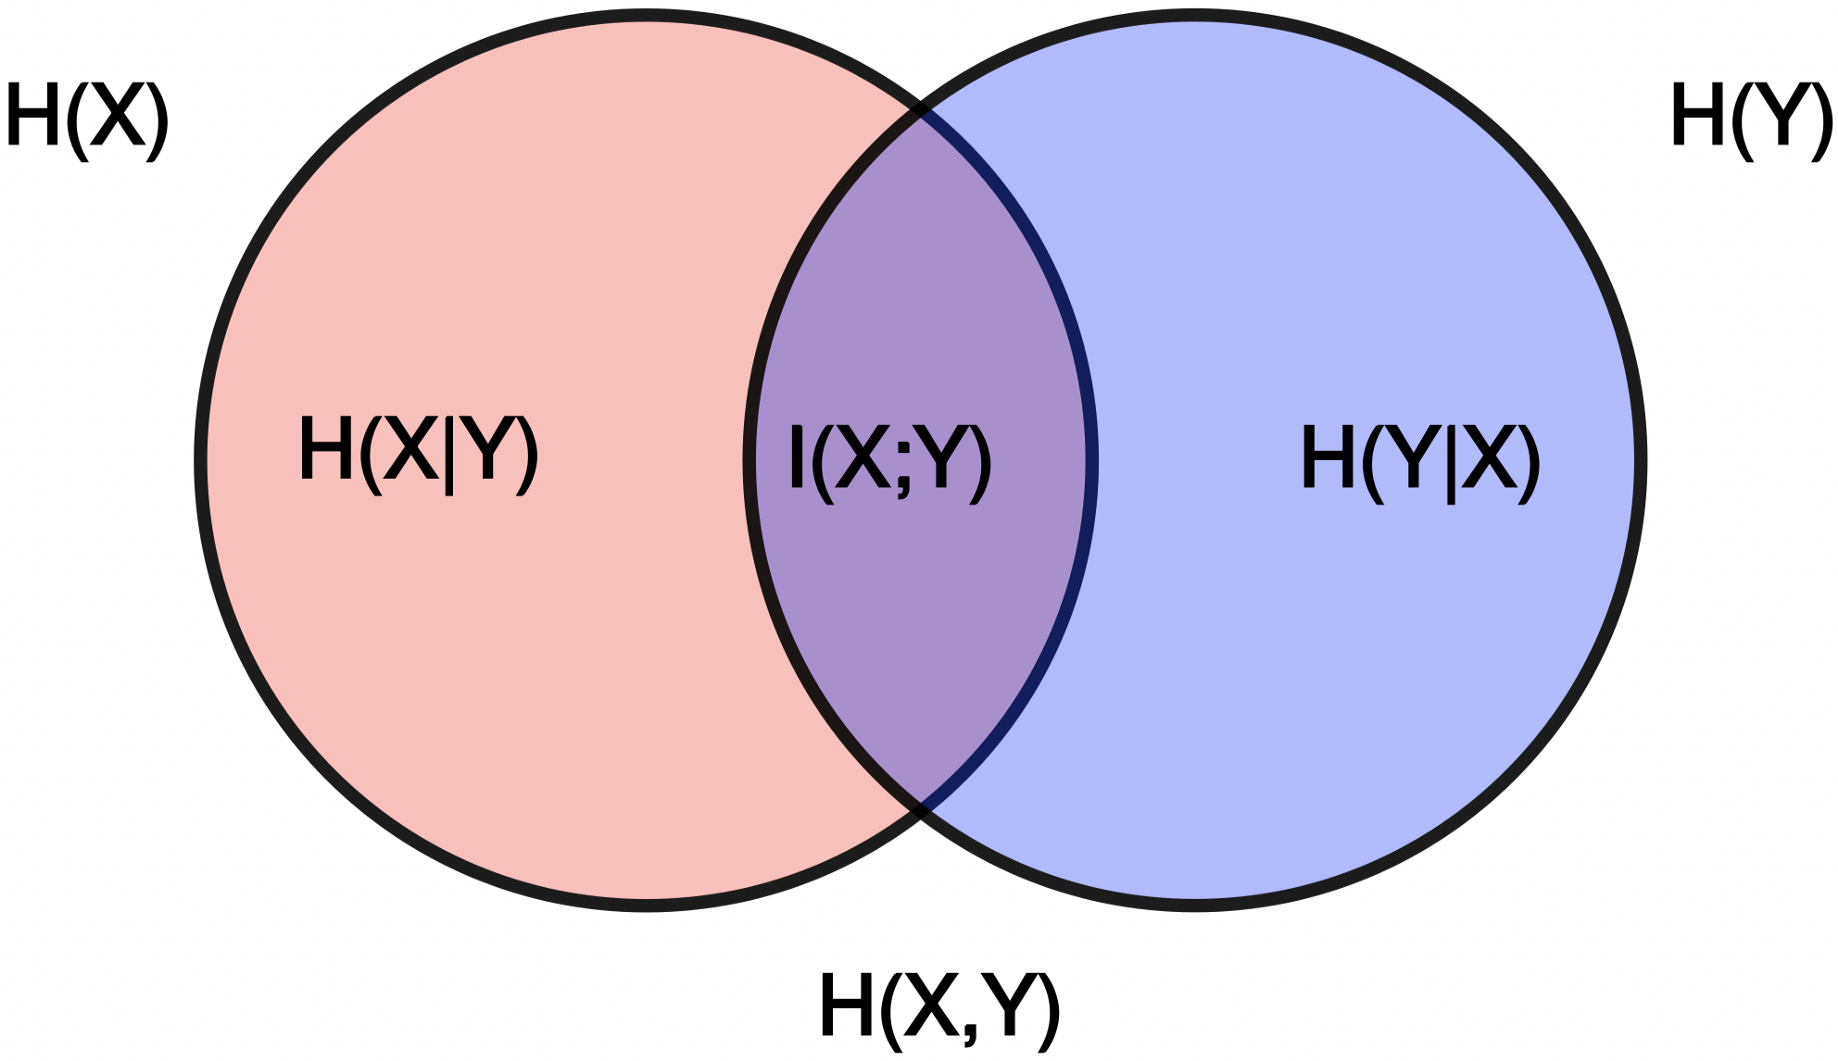
\includegraphics[width=0.7\columnwidth]{img/relationentropy.png}
    \caption{Relación entre $H$ e $I$}
    \label{fig:relationentropy}
\end{figure}

\subsection{Divergencia de Kullback-Leibler}

\begin{definition}[Divergencia de Kullback-Liebler]
Para dos densidades de probabilidad $f$ y $g$, definidas sobre un mismo conjunto de partida $\cX$, la divergencia de Kullback-Leibler entre ellas está definida mediante 
\begin{equation}
	\KL{f}{g} = \int_\cX f(x)\loga{\frac{f(x)}{g(x)}}\dx.
\end{equation}
\end{definition}

\begin{remark} La divergencia KL es siempre positiva $\forall f,g$ (desigualdad de Gibbs):
\begin{align*}
 	-\KL{f}{g}  &= \int_\cX f(x)\loga{\frac{g(x)}{f(x)}}\dx\\
 				&\leq \loga{\int_\cX f(x)\frac{g(x)}{f(x)}}\dx, \quad\quad \text{(Jensen's)}\\
 				&= \loga{\int_\cX g(x)}\dx\\
 				&=\log 1=0.,	
 \end{align*} 
Además, como $\log(\cdot)$ es estrictamente convexo, la igualdad $\KL{f}{g}=0$ solo se cumple si el argumento $\frac{g(x)}{f(x)}$ es constante, lo cual se tiene solo para ${g(x)} = {f(x)}$.
\end{remark}

Otra propiedad clave de la divergencia KL es que puede ser infinita y es asimétrica, por esta razón nos referimos a KL como divergencia y no \emph{distancia}. La intuición detrás de la KL es que es una medida de \textit{error} de estimar la densidad $f$ mediante la densidad $g$. Algunas propiedades son las siguientes:

\begin{prop}
\begin{enumerate}
    \item Relación con la información mutua:
    \[I(X;Y)=KL(p_{X,Y}||p_X p_Y)\]
\end{enumerate}
\end{prop}


\subsection{Data Processing Inequality}

\begin{theorem}[Data Processing Inequality (DPI)]
Sea una cadena de markov dada por las variables aleatorias $X\rightarrow Y\rightarrow Z$, se tiene que:

\[I(X;Y)\geq I(X;Z)\]

la cual se llama Data Processing Inequality (DPI), con igualdad si y solo si $X\rightarrow Z\rightarrow Y$ es una cadena de Markov
\end{theorem}

Como corolario directo de la DPI, se tiene que para cualquier función determinista $g(\cdot)$ se cumple que:

\[I(X;Y)\geq I(X;g(Y))\]

y entonces no existe ninguna función de $Y$ la cual pueda aumentar la información que $Y$ contiene sobre $X$.


 









\chapter{Primeros Conceptos}

\section{Modelos estadísticos}

En este curso, en particular, nos enfocaremos en  \emph{estadística matemática}, lo cual provee inferencia estadística formal basada en herramientas de probabilidades, álgebra y teoría de la medida. Para esto asumiremos que tenemos datos generados desde un modelo estadístico (o probabilístico, o \emph{generativo}) desconocido, donde nuestro objetivo es usar estos datos para determnar dichos modelos con el fin 
último de aprender sobre el mecanismo subyacente de la generación de datos y hacer predicciones (usando el modelo aprendido). El primer paso para lograr este objetivo es definir el \emph{Modelo Estadístico}.

\begin{definition} [Modelo estadístico]
Un modelo estadístico es un conjunto de distribuciones de probabilidad, que pueden ser consideradas como \emph{candidatas} para el mecanismo de generación de datos. 
\end{definition}

En algunos casos, las distribuciones de ese conjunto pueden ser expresadas mediante parámetros, por ejemplo, en el caso de la distribución normal, expresada mediante su media y su varianza. En dichos casos, el objetivo  de descubrir el mecanismo de generación de datos (la distribución) es simplemente descubrir sus parámetros.  El objetivo entonces de definir el modelo estadístico (paramétrico o no) es delinear los posibles representaciones para el mecanismo de generación de datos y, en base a los datos y algún criterio de eficiencia, encontrar el(los) modelo(s) apropiado(s). En este contexto, antes de encontrar ese modelo, consideramos que nuestro modelo tiene \emph{parámetros desconocidos.}

En el trayecto del curso, asumiremos que disponemos de un conjunto de datos $x$, que pertenece a un espacio abstracto $\mathfrak{X}$, donde típicamente $\mathfrak{X} = \mathbb{R}^n$; aunque también podremos tener datos funcionales, como por ejemplo $\mathfrak{X} = \{f:[0,1]\rightarrow \mathbb{R} \}$. Asumiremos entonces  que $x$ es la realización de una variable aleatoria $X\in\mathfrak{X}$; con lo que implícitamente asumimos que $\mathfrak{X}$ es un espacio medible con su respectiva $\sigma$-álgebra. Podemos entender nuestro modelo estadístico como el espacio de posibles hipótesis que explican los datos observados. En este sentido, una de las preguntas que debemos poder responder es ¿Cuál es la ley de X?, es decir, ¿ Cómo calcular $\mathbb{P} (X\in A)$ donde $A \in \beta (\mathfrak{X})$?, con $\beta (\mathfrak{X})$ los borelianos de $\mathfrak{X}$

Nos enfocaremos en modelos paramétricos, con lo cual para es necesario definir formalmente los parámetros y el espacio de éstos.

\begin{definition}[Parámetro y Espacio de Parámetros] 
En un problema de inferencia estadística, la (o las) característica(s) que determinan la distribución de las variables aleatorias estudiadas son llamadas parámetros. El conjunto $\Omega$ de todos los posibles valores de los parámetros se llama espacio de parámetros.
\end{definition}

Regresando a la pregunta, no habrá una, sino muchas posibles medidas de probabilidad como candidatas a ser la ley de ${X}$. A esto nos referíamos arriba cuando mencionamos la familia paramétrica de probabilidades donde cada una de las cuales puede ser la que actúa para generar $x$ a través de ${X}$. Encontrar la (o las) distribuciones, dentro de este conjunto, que son mas representativas de haber generados los datos, es un objetivo de inferencia estadística. 

Denotaremos a la familia paramétrica $\mathcal{P}$ de la siguiente forma:
\[\mathcal{P} = \{\mathcal{P}_\theta | \theta \in \Omega, \}\]
donde $\mathcal{P}_\theta $ es una medida de probabilidad bajo un parámetro $\theta \in \Omega$ en el espacio de parámetros. En nuestro estudio (pero en general no tiene que ser así) consideraremos que $\Omega$ es finito dimensional, es decir, $\Omega \subseteq \mathbb{R}^n$. Escribimos entonces que:
\[\theta = (\theta_1, ..., \theta_n). \]


Dado todo lo anterior, en la formulación de un modelo estadístico completo para representar un fenómeno se debiese tener lo siguiente plenamente identificado lo siguiente:

\begin{itemize}
    \item $\theta$ como parámetro a estimar
    \item $\Omega$ espacio de parámetros con $\Omega \subseteq \mathbb{R}^n$
    \item $\mathcal{P}_\theta$ probabilidad sobre $\mathfrak{X}$ (como función de $\theta$)
    \item ${X}$ vector aleatorio con valores en $\mathfrak{X}$
    \item $x$ elemento genérico de $\mathfrak{X}$ y realización de $X$ (datos).
\end{itemize}

\begin{example}[Fábrica de computadores]
Una compañía de fabricación de computadores desea estimar el tiempo de vida de un componente particular en sus computadores. Para ello, en primer lugar se recolectan datos de los computadores que se han usado bajo condiciones normales. Luego de ser asesorados por expertos, deciden usar una distribución normal para modelar el tiempo que se demorará un componente en fallar. Se busca modelar todos los componentes con un tiempo de vida promedio $\theta$ y varianza $\sigma
^2$, con $\theta$ y $\sigma^{2}$  parámetros desconocidos. Si se tienen $N$ componentes, las variables aleatorias que modelan la vida útil de cada componente serán identificadas como 
$X_1,..X_N$, con $X_i \sim \mathcal{N}(\theta,\sigma^{2})$. ¿Qué opina de este modelo?
\end{example}

La inferencia estadística es una herramienta que nos permitirá resolver muchos tipos de problemas. Los más importantes serán los de \emph{identificación}, donde nuestro objetivo es descubrir el modelo que genero los datos, y \emph{predicción} donde se intenta estimar una cantidad que no ha sido observada aún. Por supuesto, buscamos alcanzar ambos objetivos de forma estadística, es decir,  modelando apropiadamente la incertidumbre asociada.


%\section{Modelos estadísticos de una muestra}

\section{Construcción de variables aleatorias mediante transformaciones}

\subsection{Chi-Cuadrado}

Sean $Z_1,..., Z_n$ variables aleatorias con $Z_i\sim\mathcal{N}(0,1)$ independientes, se tiene que la suma de sus cuadrados 
\[Q=\sum\limits_{i=1}^{n} Z_i^2\]
distribuye según una distribución \textit{Chi-Cuadrado} con n grados de libertad. Esto lo denotamos como:

\[Q\sim\mathcal{X}^2_n \]
Algunas propiedades de esta distribución:
\begin{enumerate}
    \item [a.] $\mathbb{E}(\mathcal{X}^2_n) = n$
    \item [b.] $\mathbb{V}(\mathcal{X}^2_n) = 2n$
    \item [c.] $M_{\mathcal{X}^2_n}(t) = (1-2t)^{\frac{-n}{2}}$ con $t<\frac{1}{2}$
    
\end{enumerate}

\subsection{T-Student}

Sea $X_1,...,X_n$ una muestra i.i.d de una variable aleatoria $X\sim\mathcal{N}(\mu,\sigma^2)$. Consideremos el promedio muestral:
\[\overline{X}_n=\dfrac{1}{n}\sum\limits_{i=1}^n X_i\]
y la varianza muestral insesgada:
\[S^2=\dfrac{1}{n-1}\sum\limits_{i=1}^n (X_i-\overline{X}_n)^2\]

Entonces:
\[\dfrac{\overline{X}_n-\mu}{S/\sqrt{n}}\sim t_{n-1}\]
siendo $t_{n-1}$ la distribución t-student con $n-1$ grados de libertad.

\input{capitulos/Estadísticos}\clearpage

%!TEX root = ../notas_de_clase.tex


\chapter{Estimadores}


Recordemos que, dada una familia de modelos estadísticos y datos que asumimos vienen de un miembro de dicha familia, nuestro objetivo es obtener (estimar) el modelo particular que generó los datos, es decir, cuáles son los parámetros del modelo. En este capítulo se introducirá la noción de estimador, es decir, una función que busca estimar el parámetro mencionado anteriormente en base a los datos disponibles.

\begin{definition}[Estimador]
    Sea $g:\Omega\rightarrow \mathbb{R}^n$  tal que $g(\theta) = (g_1(\theta),...,g_n(\theta))$ a valores en $\mathbb{R}$. Nos interesa estimar $g(\theta)$. Para estimar $g(\theta)$ usamos un \textbf{estimador} que es una función $\hat{g}:\mathfrak{X}\rightarrow g(\Omega)$ medible. Diremos que $\hat{g}(\theta)$ es la estimación de $g(\theta)$. 
    
\end{definition}

\begin{remark}
    Los estimadores son casos particulares de los estadísticos, pues son funciones de los datos que tienen por conjunto de llegada la imagen de $\Omega$ a través de $g(\cdot)$.
\end{remark}

\begin{remark}
    Los estimadores pueden ser usados para estimar el parámetro propiamente tal, en cuyo caso $g(\theta)=\theta$, o bien otras cantidades del modelo que son expresables a través de los parámetros. Por ejemplo, en el caso de un modelo Gaussiano, si bien el parámetro puede ser expresado como $\theta = [\mu,\sigma^2]$, podemos estar interesados en estimar el intervalo de confianza del 95\%, el cual está dado (aproximadamente) por 
    \begin{equation}
        g(\theta) = [\mu - 2\sigma,\mu + 2\sigma].
    \end{equation}
\end{remark}

\begin{example}[Estimador de la media Gaussiana]
	\label{ex:estimador_media}
	Consideremos $X = (X_1,\ldots,X_n)\sim\cN(\mu,\sigma^2)$. Un estimador de $g(\theta) = g(\mu,\sigma) = \mu$ es el estadístico 
	\begin{equation}
	\nonumber
		\gh(X) = \frac{1}{n}\sum_{i=1}^nX_i.
	\end{equation} 
\end{example}



\section{Estimadores insesgados} 
Recordemos que nuestros estimadores, como función de la variable aleatoria $X$, son a su vez variables aleatorias. Consecuentemente, su estudio debe considerar sus propiedades aleatorias también. El primer paso para esto es la siguiente definición que dice relación con el valor esperado del estimador y el valor de la función $g(\theta)$ que éste estima. 

\begin{definition}[Estimador insesgado]
	\label{def:estimador_insesgado}
	Sea $\ghX$ un estimador de $g(\theta)$. Este estimador es insesgado si 
	\begin{equation}
	\nonumber
		\E{\ghX} = g(\theta),
	\end{equation}
	donde el \emph{sesgo} de $\gh$ se define como 
	\begin{equation}
	\nonumber
		b_\gh(\theta) = \E{\ghX} - g(\theta).
	\end{equation}
	Se dice también que un estimador es \textbf{asintoticamente insesgado} si es que:
	\[\lim_n\E{\gh (X_1,...,X_n)} = g(\theta),\]
	es decir, si el estimador solo se convierte en insesgado al usar \emph{infinitos datos}.
\end{definition}

Los estimadores insesgados juegan un rol relevante en el estudio y aplicación de la estadística, pues nos dicen que el estimador recupera efectivamente el parámetro \emph{en promedio}. Sin embargo, uno no siempre debe poner exclusiva atención a ellos, pues el hecho que funcione en promedio no garantiza nada en cuanto a su dispersión (varianza) o cuántas muestras necesitamos para que el estimador sea confiable. 

Los siguientes ejemplos ilustran el rol del estimador insesgado en dos familias paramétricas distintas. 

\begin{example}[Estimador insesgado de la media Gaussiana]
	\label{ex:estimador_in_media}
	El estimador de $g(\theta) =  \mu$ descrito en el Ejemplo \ref{ex:estimador_media} es insesgado, en efecto: 
	\begin{equation}
	\nonumber
		\E{\ghX} = \E{\frac{1}{n}\sum_{i=1}^nX_i}	= \frac{1}{n}\sum_{i=1}^n\E{X_i}		= \frac{1}{n}\sum_{i=1}^n\mu = \mu.
	\end{equation}
\end{example}




Veamos ahora un ejemplo de un estimador \textbf{sesgado} de la varianza y cómo se puede construir un estimador insesgado en base a éste. 

\begin{example}[Pythagoras]
Consideremos una familia paramétrica $\familiaparametrica$ y denotemos por $\mu$ y $\sigma^2$ su media y su varianza respectivamente. Usando las observaciones $x_1,x_2,\ldots,x_n$, calculemos la varianza del estimador de la media, dado por $\xb = \frac{1}{n}\sum_{i=1}^n x_i$ mediante
\begin{equation}
	\label{eq:varianza_media_muestral}
 	\Vt{\xb} = \Vt{\frac{1}{n}	\sum_{i=1}^n x_i}  \underbrace{=}_{\text{i.i.d.}}  \frac{1}{n^2}	\sum_{i=1}^n\Vt{ x_i} =\frac{\sigma^2}{n},
 \end{equation} 
 es decir, el estimador de la media usando $n$ muestras, tiene una varianza $\sigma^2/n$.

 Consideremos ahora el siguiente estimador para la varianza: 
\begin{equation}
	\label{eq:est_varianza_sesgado}
	S_2 = \frac{1}{n}\sum_{i=1}^n (x_i-\xb)^2,
\end{equation}
y notemos que la esperanza de dicho estimador es
\begin{align}
	\label{eq:sesgo_varianza}
	\Et{S_2 } &= \Et{\frac{1}{n}\sum_{i=1}^n (x_i-\mu+\mu-\xb)^2}\nonumber\\
				&= \Et{ \frac{1}{n}\sum_{i=1}^n(x_i-\mu)^2 + 2\frac{1}{n}\sum_{i=1}^n(x_i-\mu)(\mu-\xb) + \frac{1}{n}\sum_{i=1}^n(\mu-\xb)^2}\nonumber\\
				&= \Et{ \frac{1}{n}\sum_{i=1}^n(x_i-\mu)^2 - 2(\mu-\xb)^2 + (\mu-\xb)^2}\nonumber\\
				&= \Et{ \frac{1}{n}\sum_{i=1}^n(x_i-\mu)^2 - (\mu-\xb)^2}\nonumber\\
				&= \Vt{x_i} - \Vt{\xb}\quad\text{ver ecuación \eqref{eq:varianza_media_muestral}}\nonumber\\
				&= 	\sigma^2 + \sigma^2/n = \left(\frac{n+1}{n}\right)\sigma^2.
\end{align}
Esto quiere decir que el sesgo del estimador en la ecuación \eqref{eq:est_varianza_sesgado} es asintóticamente insesgado, es decir, que su sesgo tiende a cero cuando el número de muestas $n$ tiende a infinito. Sin embargo, podemos corregir el estimador de la varianza multiplicando el estimador original $S_2$ en la ecuación \eqref{eq:est_varianza_sesgado}, por $n/(n+1)$, con lo que el estimador corregido denotado por 
\begin{equation}
	\label{eq:est_varianza_insesgado}
	S'_2 = \frac{n}{n+1}S_2 =  \frac{1}{n+1}\sum_{i=1}^n (x_i-\xb)^2,
\end{equation}
cumple con
\begin{equation}
	\Et{S'_2 } =  \left(\frac{n}{n+1}\right)\Et{S_2} \underbrace{=}_{\text{ec.}\eqref{eq:sesgo_varianza}} \left(\frac{n}{n+1}\right) \left(\frac{n+1}{n}\right)\sigma^2 = \sigma^2,
\end{equation}
es decir, el estimador $S'_2$ en la ecuación \eqref{eq:est_varianza_insesgado} es insesgado.
\end{example}






\section{Funciones de pérdida}

Una función de pérdida, también llamada función de costo, es una función a valores reales de dos argumentos que, intuitivamente, determina el costo de estimar uno de los argumentos mediante el otro. Como nuestro objetivo es estimar parámetros definimos entonces una función de costo de la siguiente forma. \textbf{Desde ahora consideraremos estimadores de $g(\theta) = \theta$ y todas las esperanzas serán con respecto a $\theta$ por simplicidad de notación.}

\begin{definition}[Función de costo]
Sea $\theta\in\Omega$ un parámetro y $a\in\Omega$ un estimador, entonces el costo de estimar $\theta$ mediante $a$ está dado por la función de costo definida mediante:
\begin{align}
    L: (\Omega \times \Omega) &\rightarrow \R\\
    (\theta \times a) &\mapsto L(\theta,a).
\end{align}

\end{definition}

\begin{example}[Función de costo cuadrática]
	\label{ex:costo_cuadrático}
Una función de costo ampliamente usada para comparar estimadores es el \textbf{error cuadrático}, el cual
está dado por  
$$
L_2(\theta,a) = ||\theta-a||^{2}.
$$
\end{example}
Pregunta: ¿por qué usamos el exponente igual a 2 y no otro?

\begin{example}[Función de costo $0-1$]
	\label{ex:costo_0-1}
Cuando estimamos parámetros que no tiene relación de orden, podemos usar la función de costo $0-1$ dada por
$$
L_{01}(\theta,a) = \mathbb{1}_{\theta\neq a}.
$$
\end{example}

\begin{example}[Divergencia de Kullback-Liebler]
	\label{ex:costo_KL}
Cuando los parámetros a estimar son distribuciones de probabilidad, podemos usar la siguiente función de costo
$$
L_{\text{KL}}(\theta,a) = \sum_{i=1}^D\theta_i \log\left(\frac{\theta_i}{a_i}\right).
$$
\end{example}

	
Como el estimador (que es el argumento de la función de pérdida) es una VA, también lo es la función de pérdida.  Consecuentemente, podemos calcular la esperanza de la función de pérdida, lo cual conocemos como \textit{riesgo}. 

En particular, el riesgo asociado a la pérdida cuadrática en el Ejemplo \ref{ex:costo_cuadrático} para un estimador $\phi$ del parámetro $\theta$, está dado por: 
\begin{alignat}{3}
 	R(\theta, \phi)  &= \E{(\theta - \phi)^2}\nonumber\\
 						& = \E{\left(\theta - \bar{\phi}+ \bar{\phi} -\phi\right)^2}; \quad \text{denotando }\bar{\phi} = \E{ \phi}\nonumber\\
 						& = \E{(\theta - \bar{\phi})^2+2(\theta - \bar{\phi})\cancel{(\bar{\phi} -\phi)} +  (\bar{\phi} -\phi)^2}\nonumber\\
 						& = \underbrace{(\theta - \bar{\phi})^2}_{=b_{\phi}^2\ (\text{sesgo}^2)} +  \underbrace{\E{(\bar{\phi} -\phi)^2}}_{=V_{\phi}\ \text{(varianza)}}.\label{eq:riesgo_cuad}
 \end{alignat} 
 Donde podemos ver unas de las razones de la consideración del costo cuadrático: su riesgo se divide intuitivamente en dos términos que expresan la exactitud (cuán sesgado es) y la precisión (cuán disperso es) del estimador.


\section{Teorema de Rao-Blackwell}
\textbf{Comentario:} Para una notación más clara, nos referimos  a los estimadores estimadores $\phi=\gh$ de $\theta$ en general para evitar la expresión más engorrosa estimador $\gh(X)$ de $g(\theta)$.

Siguiendo el racional de la sección anterior, evaluaremos la bondad de distintos estimadores (sesgados o insesgados) mediante una función de \textit{pérdida} o \textit{costo} que compara el valor reportado por el estimador y el valor real del parámetro. Esto permite usar la función de pérdida como una métrica para comparar (la bondad de) dos o más estimadores.\\

El siguiente teorema establece que la información reportada por un estadístico suficiente (Definición \ref{def:estadístico_suficiente}), puede solo mejorar un estimador. 

\begin{theorem}[Teorema de Rao-Blackwell]
	\label{teo:rao-blackwell}
	Sea $\phi = \phi(X)$ un estimador de $\theta$ tal que $\Et{\phi}<\infty, \forall \theta$. Asumamos que existe $T=T(X)$ estadístico suficiente para $\theta$ y sea $\phi^\star = \Et{\phi|T}$. Entonces, 
	\begin{equation}
		\Et{(\phi^\star-\theta)^2} \leq \Et{(\phi-\theta)^2}, \forall\theta,
	\end{equation}
	donde la desigualdad es estricta salvo en el caso donde $\phi$ es función de $T$.
\end{theorem}

En otras palabras, el Teo. de Rao-Blackwell establece que un estimador puede ser \textit{mejorado} si es reemplazado por su esperanza condicional dado un estadístico suficiente. El proceso de mejorar un estimador poco eficiente de esta forma es conocido como \textit{Rao-Blackwellización} y veremos un ejemplo a continuación.


\begin{example}
Consideremos $X = (X_1,\ldots,X_n)\sim \poi{\theta}$ y estimemos el parámetro $\theta$. Para esto, consideremos el estimador básico $\phi = X_1$ y \textit{Rao-Blackwellicémoslo} usando el estimador suficiente $T=\sum_{i=1}^nX_i$, es decir, 
\begin{equation}
	\phi^* = \Et{X_1\middle|\sum_i X_i=t}.
\end{equation}
Para calcular esta esperanza condicional, observemos primero que  
\begin{equation}
	\sum_{j=1}^n\Et{X_j\middle|\sum_{i=1}^n X_i=t} = \Et{\sum_{j=1}^nX_j\middle|\sum_{i=1}^n X_i=t} = t,
\end{equation}
y que como $X_1,\ldots,X_n$ son iid, entonces todos los términos dentro de la suma del lado izquierdo de la ecuación anterior son iguales. Consecuentemente, recuperamos el estimador
\begin{equation}
 	\phi^* = \frac{t}{n} = \frac{1}{n}\sum_{i=1}^nX_i.
 \end{equation} 
\end{example}

Antes de demostrar el Teorema \ref{teo:rao-blackwell} consideremos dos variable aleatorias $X\in\cX$, $Y\in\cY$, y recordemos dos propiedades básicas. En primer lugar la ley de esperanzas totales, la cual establece que 
\begin{alignat}{3}
	\mathbb{E}_Y{\mathbb{E}_{X|Y}{(X|Y)}} &= \int_\cY\int_\cX x \d P(x|y) \d P(y) \quad\quad&&\text{def. esperanza}\nonumber\\
				&=  \int_\cX x \int_\cY \d P(x|y) \d P(y) &&\text{linealidad}\nonumber\\
				&=  \int_\cX x \int_\cY \d P(x,y) &&\text{def. esperanza condicional}\nonumber\\
				&=  \int_\cX x \d P(x) = \mathbb{E}_X(X). &&\text{def. esperanza} \label{eq:total_expectation}
\end{alignat}
En segundo lugar, recordemos (?) la desigualdad de Jensen, la cual para el caso particular del costo cuadrático, puede verificarse mediante
\begin{equation}
	0 \leq \V{X} =  \E{X^2}-\E{X}^2 \Rightarrow \E{X^2} \geq \E{X}^2. \label{eq:jensen_var}
\end{equation}
La desigualdad de Jensen es geométricamente intuitiva, como se observa en la Figura \ref{fig:intuicion_jensen}. Al calcular la imagen de $\mathbb{E}(x)$ bajo una función convexa, podemos encontrar una recta tangente a ese punto $L(X)=aX+b$. Tendremos que $\mathbb{E}(\varphi(X')) \geq \mathbb{E}(L(X'))=\mathbb{E}[aX'+b]=a\mathbb{E}[X`]+b=L(\mathbb{E}(X'))$ para otro punto $X'$. Tomando $X'=X$, $\mathbb{E}(\varphi(X)) \geq \varphi(\mathbb{E}(X))$.
\begin{figure}[ht]
    \centering
    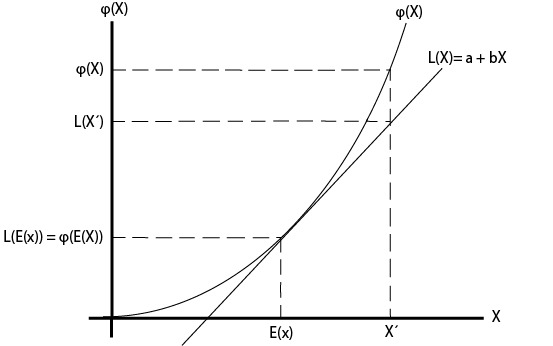
\includegraphics[scale=0.5]{img/Intuicion_Jensen.jpeg}
    \caption{Intuición geométrica de la desigualdad de Jensen }
    \label{fig:intuicion_jensen}
\end{figure}

Volviendo a lo anterior, utilizando las expresiones en \eqref{eq:total_expectation} y \eqref{eq:jensen_var}, podemos demostrar el teorema anterior.

 \begin{proof}[Demostración de Teorema \ref{teo:rao-blackwell}]
 	La varianza del estimador $\phi^\star$ está dada por 
 	\begin{alignat*}{2}
 		\Et{(\phi^\star-\theta)^2} &= \Et{(\Et{\phi|T}-\theta)^2} \quad\quad\quad &&\text{def.}\\
 								&= \Et{(\Et{\phi-\theta|T})^2}&& \text{linealidad}\\
 								&\leq \Et{\Et{(\phi-\theta)^2|T}}&& \text{Jensen}\\
 								&= \Et{(\phi-\theta)^2} &&\text{ley esperanzas totales}
 	\end{alignat*}
Donde las esperanzas exteriores son con respecto a $T$ y las interiores con respecto a $X$ (o equivalentemente a $\phi$).  Observemos además que la desigualdad anterior viene de la expresión en la ecuación \eqref{eq:jensen_var}, por lo que la igualdad es obtenida si $\V{\phi-\theta|T} = 0$, es decir, la VA $\phi-\theta$ tiene que ser constante para cada valor de $T$, es decir, $\phi$ es función de $T$. Intuitivamente podemos entender esto como que si el estadístico ya fue considerado en el estimador, entonces conocer el valor del estadístico no reporta información adicional. 
 \end{proof}

\begin{remark}
	Notemos que si el estimador $\phi$ es insesgado, su \textit{Rao-Blackwellización} $\phi^*$ también lo es, en efecto
	\begin{equation}
		\Et{\phi^*} = \Et{\Et{\phi|T}} = \Et{\phi} = \theta,
	\end{equation}
	donde la segunda igualdad está dada por la ley de esperanzas totales y la tercera por el supuesto de que $\phi$ es insesgado.
\end{remark}

\section{Varianza uniformemente mínima}

Observemos que, en base al riesgo cuadrático definido en la ecuación \eqref{eq:riesgo_cuad}, si un estimador es insesgado (Definición \ref{def:estimador_insesgado}) entonces su riesgo cuadrático es únicamente su varianza. Esto motiva la siguiente definición de optimalidad para estimadores insesgados. 

 \begin{definition}[Estimador insesgado de varianza uniformemente mínima]
  	El estimador $\phi=\phi(X)$ de $\theta$ es un estimador insesgado de varianza uniformemente mínima (EIVUM) si es insesgado y además si $\forall \phi':\cX\rightarrow \Theta$ estimador insesgado se tiene
  	\begin{equation}
  		\Vt{\phi}\leq\Vt{\phi'}, \forall \theta\in\Theta.
  	\end{equation}
  	Es decir, el EIVUM es el estimador insesgado que tiene menor varianza de todos los estimadores insesgados (y puede no ser único).
  \end{definition} 

\begin{example}
	Consideremos $X=(X_1,\ldots,X_n)\sim\ber{\theta}$ y los siguientes estimadores de $\theta$
	\begin{itemize}
		\item $\phi_1(X) = X_1$
		\item $\phi_2(X) = \frac{1}{2}(X_1+X_2)$
		\item $\phi_3(X) = \frac{1}{n}\sum_{i=1}^n X_i$
	\end{itemize}
	Observemos que todos estos estimadores son insesgados, pues como $\forall i, \Et{X_i} = \theta$, entonces 
	\begin{equation}
		\Et{\phi_1(X)} = \Et{\phi_2(X)} = \Et{\phi_3(X)} = \theta.
	\end{equation}
	Veamos ahora que la varianza de $\phi_3(X)$ está dada por
	\begin{equation}
		\Vt{\phi_3(X)} = \Vt{\frac{1}{n}\sum_{i=1}^n X_i} = \frac{1}{n^2}\sum_{i=1}^n \Vt{X_i} = \frac{\theta(1-\theta)}{n}
	\end{equation}
	pues $\Vt{X_i} = \Et{(\theta - X_i)^2} = \Et{X_i^2} - \theta^2 = (0^2 \cdot (1-\theta) + 1^2 \cdot \theta) - \theta^2 = \theta(1-\theta)$. Consecuentemente, la varianza de los estimadores considerados decae como la inversa del número de muestras $1/n$.
\end{example}

Con las definiciones anteriores, podemos mencionar el siguiente teorema, el cual conecta la noción de estadístico completo con la de EIVUM. 

\begin{theorem}[Teorema de Lehmann-Scheffé]
	Sea $X$ una VA con distribución paramétrica $\familiaparametrica$ y $T$ un estadístico suficiente y completo para $\theta$. Si el estimador $\phi = \phi(T)$ de $\theta$ es insesgado, entonces $\phi$ es el único EIVUM. 
 \end{theorem} 
 
 Es decir, el Teorema de Lehmann-Scheffé nos permite verificar que un estimador es el (único) EIVUM, si éste es insesgado y es función de un estadístico suficiente y completo. 
    

 \begin{proof}
 	Veamos en primer lugar que es posible construir un estimador en función del estadístico suficiente $\phi(T)$ que tiene menor o igual varianza que un estimador arbitrario $\phi'(X)$. En efecto, el Teorema de Rao-Blackwell establece que el estimador 
 	\begin{equation}
 		\phi(T) = \Et{\phi'(X)|T},
 	\end{equation}
 	tiene efectivamente menor (o igual) varianza que $\phi'(X)$.\\

 	Ahora veamos que solo existe un único estimador insesgado que es función del estadístico completo $T$. Asumiendo que existiesen dos estimadores insesgados de $\theta$ que son funciones de $T$, denotados $\phi_1(T),\phi_2(T)$, entonces, $\Et{\phi_1(T)-\phi_2(T)}=0$, es decir, $\phi(T) = \phi_1(T)-\phi_2(T)$ es un estimado insesgado de 0. Luego, como $T$ es completo, entonces, $\phi(T)=0$ es identicamente nulo, lo cual implica que  $\phi_1(T) = \phi_2(T)$ c.s.-$P_\theta$.\\

 	Hemos probado que (i) para un estimador arbitrario, se puede construir un estimador que es función de $T$ el cual tiene menor o igual varianza que el estimador original y, (ii) el estimador insesgado $\phi(T)$ es único. Consecuentemente, $\phi(T)$ es el único EIVUM.
 \end{proof}

El Teorema de Lehmann-Scheffé da una receta para encontrar el EIVUM: simplemente es necesario encontrar un estadístico completo y construir un estimador insesgado en base a éste, esto garantiza que el estimador construido es el \textbf{único} EIVUM.
\begin{example}[EIVUM para Bernoulli]
	Recordemos que en el Ejemplo \ref{eq:est_completo_bernoulli} vimos que el estadístico $T=\sum_{i=1}^nX_i$ es completo para $X\sim\ber{\theta}$. Como el estimador de $\theta$ dado por $\phi(T) = T/n$ es insesgado, 
\begin{equation}
	\Et{\phi(T)} = \Et{T/n} = \sum_{i=1}^n \Et{X_i} /n = \theta,
\end{equation}
entonces $\phi(T) = T/n$ es el EIVUM para $\theta$ en $\ber{\theta}$ y es único.	
\end{example}

\begin{remark}
Lectura personal: Estadístico auxiliar (ancilliary) y teoremas de Basur y de Bahadur. 
\end{remark}

\begin{definition}
Un estadístico T=T(X) se dice \textbf{ancilario} si su distribución no depende del parámetro a estimar.
\end{definition}

\begin{theorem}[Teorema de Basu]
Si T es completo y suficiente para $\theta$ y V es ancilario para $\theta$, entonces T y V son independientes
\end{theorem}


\subsection{Información de Fisher}

Para entender esta propiedad, primero definamos la función de puntaje o \textit{score function} como la {función aleatoria} definida por la derivada de la log-verosimilitud, es decir, 
\begin{equation}
	S_\theta(X) = \frac{\partial \log p_\theta(X)}{\partial\theta}.
\end{equation}

\begin{remark}
La esperanza de la función de puntaje cero. En efecto, derivando la igualdad fundamental $1 = \int_\cX p_\theta(x)\dx$ con respecto a $\theta$, obtenemos 
\begin{align}
	0 = \int_\cX \frac{\partial  p_\theta(X)}{\partial\theta} \dx = \int_\cX \frac{1}{p_\theta(X)}\frac{\partial  p_\theta(X)}{\partial\theta} p_\theta(X) \dx = \int_\cX \frac{\partial \log   p_\theta(X)}{\partial\theta} p_\theta(X) \dx = \Et{S_\theta(X)}
\end{align}
Sorprendente. 
\end{remark}

Además, veamos que al derivar por segunda vez la función de puntaje, obtenemos: 
\begin{align*}
	0 &= \int_\cX \frac{\partial}{\partial \theta }\left(\frac{\partial \log   p_\theta(X)}{\partial\theta} p_\theta(X) \right)\dx\\ 
	&= \int_\cX \left(\frac{\partial^2 \log   p_\theta(X)}{\partial\theta^2} p_\theta(X) + \frac{\partial \log   p_\theta(X)}{\partial\theta}\frac{\partial   p_\theta(X)}{\partial\theta}  \right)\dx\\
	&= \Et{\frac{\partial^2 \log   p_\theta(X)}{\partial\theta^2}} + \Et{\left(\frac{\partial \log   p_\theta(X)}{\partial\theta}\right)^2}.
\end{align*}
Cada uno de los dos términos de la ecuación anterior tiene la misma magnitud (uno es negativo y el otro es positivo), lo cual motiva la siguiente definición.

\begin{definition}[Información de Fisher]
La cantidad denotada mediante  
\begin{equation}
		I(\theta) = \Et{\left(\frac{\partial \log   p_\theta(X)}{\partial\theta}\right)^2} = 	-\Et{\frac{\partial^2 \log   p_\theta(X)}{\partial\theta^2}},
\end{equation}	
es conocida como información de Fisher. Además, como la esperanza de la función de puntaje es cero, la varianza de $I(\theta)$ puede ser expresada como 
\begin{equation}
	\Vt{S_\theta(X)} = \Et{S_\theta(X)^2} - \cancel{\Et{S_\theta(X)}^2} = \Et{\left(\frac{\partial \log   p_\theta(X)}{\partial\theta}\right)^2}.
\end{equation}
Consecuentemente, la información de Fisher también es la varianza de la función de pérdida, con lo que contamos con tres expresiones para poder calcular $I(\theta)$. 
\end{definition}

\begin{exercise}[Cálculo de la información de Fisher para Bernoulli]
	Consideremos $X\sim\ber{\theta}$, entonces, 
	\begin{align}
		I(\theta) &= -\Et{\frac{\partial^2}{\partial\theta^2}\loga{\theta^X(1-\theta)^{1-X}}}\nonumber\\
		&= -\Et{\frac{\partial^2}{\partial\theta^2} X\log\theta + \frac{\partial^2}{\partial\theta^2} 	(1-X)\loga{1-\theta}	}\nonumber\\
		&= \Et{X\theta^{-2} + (1-X)(1-\theta)^{-2}	}\nonumber\\
		&= \theta^{-1} + (1-\theta)^{-1}	\nonumber\\
		&= 	\frac{1}{\theta(1-\theta)}.
	\end{align}
\end{exercise}

\begin{exercise}[Cálculo de la información de Fisher para Poisson]
	Consideremos $X\sim\poi{\theta}$, entonces, 
	\begin{align}
		I(\theta) &= \Et{\left(\frac{\partial}{\partial\theta}\loga{\frac{\theta^Xe^{-\theta}}{X!}}\right)^2}\nonumber	\\
		&= \Et{\left( \frac{\partial}{\partial\theta}X\log\theta - \frac{\partial}{\partial\theta}\theta - \frac{\partial}{\partial\theta}\log(X!)\right)^2}\nonumber\\
		&= \Et{\left( X\theta^{-1} - 1\right)^2}\nonumber	\\
		&= \Et{ X^2\theta^{-2} -2X\theta^{-1}+ 1}\nonumber	\\
		&= (\theta+\theta^2)\theta^{-2} -2\theta\theta^{-1}+ 1\nonumber\\
		&= \theta^{-1}.\nonumber	
	\end{align}
\end{exercise}

Hasta ahora hemos calculado la función de puntaje en base a la verosimilitud de solo una una variable aleatoria. Si considerásemos la verosimilitud evaluada calculada para un conjunto de observaciones (IID), tenemos que
\begin{equation}
	S_\theta(X_1,\ldots,X_n) = \frac{\partial \log \prod_{i=1}^np_\theta(X_i)}{\partial\theta} = \sum_{i=1}^n\frac{\partial \log p_\theta(X_i)}{\partial\theta}= \sum_{i=1}^n S_\theta(X_i).
\end{equation}
De igual forma, para la información de Fisher, tenemos, 
\begin{equation}
	I_n(\theta) = \Vt{\sum_{i=1}^n S_\theta(X_i)} = n I(\theta).
\end{equation}
\begin{remark}
La expresión anterior confirma la intuición sobre la información de Fisher en cuanto a \emph{cuán informativa} es una muestra $X$ para estimar el parámetro $\theta$: Si una muestra tiene tiene una información de Fisher $I(\theta)$, entonces $n$ muestras independientes del mismo modelo tendrán  $n$ veces dicha información. 
\end{remark}

\subsection{Cota de Cramer Rao}

Veamos ahora una desigualdad interesante para la información de Fisher y su relación con estimadores. Consideremos un estimador insesgado, es decir, 
\begin{equation}
	\Et{\hat{\theta}(X)-\theta}=\int_\cX (\hat{\theta}(X)-\theta)p_\theta(X)\dx=0.
\end{equation}
Derivando esta expresión con respecto a $\theta$, obtenemos

\begin{align*}
	0 &= \frac{\partial}{\partial\theta}\int_\cX (\hat{\theta}(X)-\theta)p_\theta(X)\dx\\
	  &= -\int_\cX p_\theta(X)\dx  + \int_\cX (\hat{\theta}(X)-\theta)\frac{\partial p_\theta(X)}{\partial\theta}\dx\\
	  &= -1  + \int_\cX (\hat{\theta}(X)-\theta)\frac{\partial\log p_\theta(X) }{\partial\theta}p_\theta(X)\dx.
\end{align*}
Lo que implica que 
\begin{align*}
	1 &= \left(\int_\cX (\hat{\theta}(X)-\theta)\frac{\partial\log p_\theta(X) }{\partial\theta}p_\theta(X)\dx\right)^2\\
	&=\left(\int_\cX (\hat{\theta}(X)-\theta)\sqrt{p_\theta(X)}\sqrt{p_\theta(X)}\frac{\partial\log p_\theta(X) }{\partial\theta}\dx\right)^2\\
	&\leq\int_\cX (\hat{\theta}(X)-\theta)^2 p_\theta(X)\dx \int\left(\frac{\partial\log p_\theta(X) }{\partial\theta}\right)^2 p_\theta(X)\dx.
\end{align*}
Notemos que la primera integral es la varianza del estimador insesgado $\hat\theta$ y la segunda es la esperanza del cuadrado de la función de puntaje (o la información de Fisher). Con esto, podemos enunciar el siguiente resultado 
\begin{definition}[Cota de Cramer-Rao]
	Sea $X_1,\ldots,X_n \sim p_\theta$ y $nI(\theta)$ su información de Fisher. Entonces para todo estimador insesgado $\theta'$ tenemos 
	\begin{equation}
		\Vt{\theta'}\geq (nI(\theta))^{-1},\quad \forall \theta\in\Theta
	\end{equation}
\end{definition}
La cota de Cramer-Rao es un elemento fundamental en el estudio estadístico, pues establece que cualquier estimador insesgado tiene necesariamente una varianza que está por sobre el recíproco de la información de Fisher. Es decir, la varianza de un EIVUM se encuentra acotada inferiormente.


\section{Completitud}

Otra propiedad de los estimadores que permite estudiar su capacidad de estimar es la de \textit{completitud}. A continuación definimos esta propiedad para el caso general de un estadístico, no necesariamente un estimador.

\begin{definition}[Estadístico completo]
	Un estadístico $T(X)$ es completo si para toda función $f$, se tiene que 
	\begin{equation}
		\Et{f(T)|\theta} = 0, \forall \theta\in\Theta \Rightarrow \Probt{f(T)=0} = 1, \forall \theta\in\Theta.
	\end{equation}
	
\end{definition}



Intuitivamente entonces, podemos entender la noción de completitud como lo siguiente: un estadístico es completo si la única forma de construir un estimador insesgado de cero a partir de él es aplicándole la función idénticamente nula.  Veamos un ejemplo de la distribución Bernoulli, donde el estadístico $T(x) = \sum x_i$ es efectivamente completo. 

\begin{example}
	\label{eq:est_completo_bernoulli}
	Sea $x=(x_1,\ldots,x_n)$ observaciones de $X\sim\ber{\theta}$, recordemos que $T(x) = \sum x_i\sim\bin{n,\theta}$, por lo que la esperanza de $f(T)$ está dada por
	\begin{equation}
		\Et{f(T)} = \sum_{t=0}^n f(t)\binom{n}{t}\theta^t(1-\theta)^{n-t}= (1-\theta)^n\sum_{t=0}^n f(t)\binom{n}{t}\left(\frac{\theta}{1-\theta}\right)^t,
	\end{equation}
	es decir un polinomio de grado $n$ en $r=\theta/(1-\theta)\in\R_+$. Entonces, $\Et{f(T)} = 0,\forall\theta$, implica que necesariamente los pesos de este polinomio son todos idénticamente nulos, es decir, $f(t)=0,\forall t$, lo que a su vez implica $\Probt{f(T)=0} = 1$. Consecuentemente, $T(x) = \sum x_i\sim\bin{n,\theta}$ es un estadístico completo.
\end{example}

El concepto de completitud dice relación con la construcción de estimadores usando estadísticos, lo cual puede ser ilustrado mediante el siguiente ejemplo

\begin{example}
	Consideremos dos estimadores, $\phi_1, \phi_2$ insesgados de $\theta$ distintos, es decir, 
	\begin{equation}
	\E{\phi_1} = \E{\phi_2} = \theta, \ \Prob{\phi_1\neq \phi_2} > 0.
	\end{equation}
	Definamos ahora $\phi = \phi_1 - \phi_2$, donde verificamos que $\E{\phi} = 0, \forall \theta$, es decir, $\phi$ es un estimador insesgado de cero. Como nuestra hipótesis en la ecuación anterior dice que $\Prob{\phi_1 - \phi_2=0}>0$, de acuerdo a la definición  de estadístico completo, $\phi$ no es completo. 
\end{example}


\begin{example}[Estimador de la taza de la distribución exponencial]
	\label{ex:estimador_exponancial}
	Consideremos $X\sim Exp(\theta)$, donde $Exp(x|\theta) = \theta\exp(-\theta x),\theta>0$. Veamos en primer lugar que el estadístico trivial $T(X) = X$ es completo. En efecto, para una función cualquiera $f(\cdot)$, como $\theta>0$ tenemos
	\begin{equation}
	    \Et{f(X)} = \int_0^\infty f(x)\theta\exp(-\theta x)\d x = 0 \Rightarrow  \int_0^\infty f(x)\exp(-\theta x)\d x = 0
	\end{equation}
	con lo cual si el lado derecho de la expresión anterior se cumple  $\forall \theta$, entonces necesariamente $f(x)=0$ (¿por qué?).
	
	En segundo lugar, asumamos que existe un estimador insesgado $\ghX$ de $g(\theta) = \theta$. Es decir, 
	\begin{equation}
	\nonumber
		\Et{\ghX} = \int_0^\infty \ghx\theta\exp(-\theta x)\d x = \theta, \forall \theta,
	\end{equation}
	lo cual es equivalente a $\int_0^\infty \ghx\exp(-\theta x)\d x = 1, \forall \theta$, y también a (al derivar ambos lados de esta expresión c.r.a. $\theta$) 
	\begin{equation}
	    \int_0^\infty x\ghx\exp(-\theta x)\d x = 0, \forall \theta.
	\end{equation}

	Esta última expresión es equivalente a que $\E{X\ghX} = 0$, con lo que podemos utilizar el hecho de que $X$ es un estadístico completo para decir que la función $X\ghX=0$ c.s. $\forall \theta$, y consecuentemente $\ghX=0$ c.s. $\forall \theta$. 
	
	Hemos mostrado que el supuesto de la existencia de un estimador (denotado $\ghX$) insesgado para el parámetro del modelo exponencial $\theta>0$, resulta en la contradicción $\ghX=0$ c.s. Consecuentemente, no es posible construir estimadores insesgados para $\theta$ en la distribución exponencial.
\end{example}

\section{Ejercicios}

\begin{enumerate}

\item Considere una Muestra Aleatoria Simple (MAS) $X=(X_1,...,X_n)$ donde $X_i\sim\mathcal{N}(\mu, \sigma^2)$, $\forall i =1,...,n$ con $\mu$ y $\sigma$ son parámetros desconocidos. Se consideran al estimador de la varianza y la media como:

\[S^2 := \frac{1}{n-1}\sum\limits_{i=1}^{n}(\overline{X}_n-X_i)^2, \quad \hat{\mu} := \overline{X}_n \]
donde $\overline{X}_n$ denota al promedio de $X_1,..., X_n$, es decir  $\overline{X}_n = \frac{1}{n}\sum\limits_{i=1}^{n}X_i$. 

\begin{enumerate}
    \item Demuestre que $S^2$ y $\hat{\mu}$ son independientes.
\end{enumerate}

\item Sea $X=(X_1,...,X_n)$ una MAS de un modelo Poisson de parámetro $\lambda$. Se busca estimar insesgadamente la función generadora de momentos $M_{X}(t)=\mathbb{E}[e^{tX}]$. Para esto, siga los siguientes pasos:

\begin{enumerate}
    \item Muestre que $M_{X_i}(t)=e^{-\lambda (1-e^t)}$, con $t\in \mathbb{R}$
    \item Compruebe que $\widehat{M_{X}}(t)=e^{t X_1}$ es un estimador insesgado de $M_{X}(t)$.
    \item Muestre que el estadístico $T(X)=\sum\limits_{i=1}^{n}X_i$ tiene ley Poisson de parámetro $n \lambda$.
    \item Calcule $\mathbb{P}(X_1 =k | S=s)$. ¿Qué ley sigue?
    \item Muestre que $T(X)$ es un estadístico suficiente y completo para $\lambda$
    \item Encuentre el estimador EIVUM para $M_{X}(t)$
\end{enumerate}

\item Sea una MAS $X=(X_1,..,X_n)$ con n observaciones independientes del modelo gaussiano $\mathcal{N}(\mu,\sigma^2)$ y otra MAS $Y=(Y_1,...Y_n)$ con n observaaciones independientes del modelo gaussiano $\mathcal{N}(\nu,\sigma^2)$. Se supone que X e Y son vectores independientes y que los parámetros $\mu,$ $\nu$, $\sigma$ son desconocidos y no están sujetos a ninguna restricción.

\begin{enumerate}
    \item Plantee el modelo paramétrico relacionado a la situación planteada. Compruebe $\mathcal{P}$ pertenece a la clase exponencial y que es de rango completo en la parametrización natural.
    \item Analice los siguientes estadísticos e indique si son suficientes y/o minimales:
    \begin{itemize}
        \item $T_1=\left (\sum\limits_{i=1}^{n}X_i,\sum\limits_{i=1}^{n}Y_i,\sum\limits_{i=1}^{n}X^2_i,\sum\limits_{i=1}^{n}Y^2_i  \right )$
        \item $T_2=\left (\sum\limits_{i=1}^{n}X_i,\sum\limits_{i=1}^{n}Y_i,\sum\limits_{i,j=1}^{n}Y_iX_j  \right )$
        \item $T_3=\left (\sum\limits_{i=1}^{n}(X_i+Y_i),\sum\limits_{i=1}^{n}X_i^2,\sum\limits_{i,j=1}^{n}Y^2_i  \right )$
    \end{itemize}
    \item Muestre que $S=\left (\sum\limits_{i=1}^{n}X_i,\sum\limits_{i=1}^{n}Y_i,\sum\limits_{i,j=1}^{n}Y^2_i+X^2_i  \right )$ es un estadístico suficiente completo para $\mathcal{P}$
    \item Encuentre el EIVUM para las siguientes funciones del parámetro $\theta$:
    \begin{itemize}
        \item $g_1(\theta)=\mu +\nu$
        \item $g_2(\theta)=\mu\nu$
        \item $g_3(\theta)=\sigma^2$
    \end{itemize}
    
    
    
    
\end{enumerate}



Se suele presentar cuando un vector bidimensional (por ejemplo, el que representa la velocidad del viento) tiene sus dos componentes, ortogonales, independientes y siguen una distribución normal. Su valor absoluto seguirá entonces una distribución de Rayleigh

\item Sea $X=(X_1,...,X_n)$ una MAS de $n\in \mathbb{N}$ observaciones con $X_n\sim Unif(\theta,2\theta)$. Considere que para la MAS anterior, sus estadísticos de orden $X_{(1)},...,X_{(n)}$ poseen una densidad dada por:

\[ f_{X_{(i)}}(x)=\frac{n!}{(i-1)!(n-i)!}\frac{1}{\theta}\left (\frac{x-\theta}{\theta}  \right )^{i-1}\left (1-\left (\frac{x-\theta}{\theta}  \right )  \right )^{n-i}\quad, \quad x\in[\theta,2\theta]. \]

Se busca estimar el parámetro $\theta$. Para esto se pide lo siguiente:
\begin{enumerate}
    \item Encuentre un estadístico suficiente para $\theta$.
    \item Considere el estimador $\hat{\theta}=\frac{2}{3}X_1$. Muestre que es insesgado.
    \item Utilice el Teorema de Rao-Blackwell para encontrar un estimador $\widetilde{\theta}$ de $\theta$ con menor MSE que $\hat{\theta}$. 
    \item Demuestre que $\widetilde{\theta}$ es insesgado.
    \item Interprete $\widetilde{\theta}$
\end{enumerate}
\end{enumerate}



\chapter{Construcción de estimadores}

\section{Estimador de Máxima Verosimilitud (EMV)} % (fold)
\label{sec:estimador_de_máxima_verosimilitud}

Informalmente, el estimador de un parámetro es una función de los datos que deseamos que entregue un valor cercano al parámetro. Dada una cantidad desconocida, se hace natural la idea de buscar encontrar una \emph{buena} (y ojalá la \emph{mejor}) función de los datos que nos permita estimarla, pero ¿Qué significa que un estimador sea un buen estimador?

Dado que el parámetro $\theta$ es desconocido, calcular la distancia de un estimador $\hat\theta = \hat\theta(X)$ a este no es posible, pues de lo contrario  podríamos simplemente utilizar una función de pérdida como las definidas en el capítulo anterior.

En esta sección, veremos cómo construir estimadores usando directamente la densidad de probabilidad de la VA $X\in\cX$, donde aparece el parámetro $\theta$ y una colección de datos (o realizaciones del modelo). Para este fin la función de verosimilitud en la definición \ref{función_verosimilitud} será fundamental. Recordemos que la función de verosimilitud (del parámetro $\theta$ dados los datos $X$) es la densidad de probabilidad de los datos $X$ si el valor del parámetro fuese efactivamente $\theta$. Consecuentemente, la verosimilitud permite encontrar un estimador en base a una métrica clara: cuan probable es cada estimador de haber generado los datos. Esto da las condiciones para determinar un estimador que recibe mucha atención en la literatura estadística: 

\begin{definition}[Estimador de máxima verosimilitud (MV)]
	Sea una observación $x$ y una función de verosimilitud $L(\theta)$, el estimador de máxima verosimilitud está dado por 
	\begin{equation}
		\thetaMV = \underset{\theta}{\arg\max}\ L(\theta|x)
	\end{equation}	
\end{definition}

Claramente, el estimador de MV puede ser definido con respecto a la verosimilitud o a cualquier función no decreciente de ésta, como también pude no existir o no ser único. En particular, nos enfocaremos en encontrar $\thetaMV$ mediante la maximización de la log-verosimilitud $l(\theta) = \log L(\theta)$, la cual es usualmente más fácil de optimizar en términos computacionales o analíticos. De hecho, muchas veces incluso ignoraremos constantes de la (log) verosimilitud, pues éstas no cambian el máximo de $L(\theta)$.

\begin{example}[Máxima verosimilitud: Bernoulli]
	\label{ex:bernoulli_MV}
	Sea $X_1,\ldots X_n\sim\ber{\theta}$, la verosimilitud de $\theta$ está dada por 
	\begin{equation}
		L(\theta) = \prod_{i=1}^n\theta^x_i(1-\theta)^{1-x_i},
	\end{equation}
	y su log-verosimilitud por $l(\theta) = (\sum_{i=1}^nx_i)\log \theta + (n-\sum_{i=1}^nx_i)\log(1-\theta)$. El estimador de  MV puede ser encontrado resolviendo $\frac{\partial l(\theta)}{\partial \theta} = 0$:
	\begin{align*}
	\frac{\partial l(\theta)}{\partial \theta} =0 
	&\Rightarrow  (\sum_{i=1}^nx_i) \theta^{-1} = (n-\sum_{i=1}^nx_i)(1-\theta)^{-1}\\
	&\Rightarrow  \sum_{i=1}^nx_i (1-\theta) = (n-\sum_{i=1}^nx_i) \theta\\
	&\Rightarrow  \theta = \sum_{i=1}^nx_i/n.
	\end{align*}
Notemos que este estimador de MV ¡es a su vez el EIVUM!	
\end{example}


\begin{exercise}
	Graficar $l(\theta)$ en el Ejemplo \ref{ex:bernoulli_MV}.
\end{exercise}

\begin{exercise}
	Encuentre el estimador de MV de $\theta = (\mu,\Sigma)$ para la VA $X\sim\cN(\mu,\Sigma)$.
\end{exercise}

\begin{example}
	Sea la VA $X\sim\uni{\theta}$, es decir, $p(x) = \theta^{-1} \ind_{0\leq x \leq \theta}$. Para calcular la verosimilitud, recordemos en primer lugar que la verosimilitud factoriza de acuerdo a  
	\begin{equation}
		L(\theta) = \prod_{i=1}^n p_\theta(x_i)
	\end{equation}
	y observemos que necesariamente $p_\theta(x_i) = 0$ si $x_i>\theta$. Consecuentemente, $L(\theta)>0$ solo si $\theta$ es mayor que toda las observaciones, en particular, si $\theta\geq\max\{x_i\}_1^n$.

	Además, si efectivamente tenemos $\theta\geq\max\{x_i\}_1^n$, entonces notemos que $p_\theta(x_i) = 1/\theta$, por lo que la verosimilitud está dada por
		\begin{equation}
		L(\theta) = \theta^{-n}, \quad \theta\geq\max\{x_i\}_1^n
	\end{equation}
	y consecuentemente, el estimador de máxima verosimilitud es $\thetaMV = \max\{x_i\}_1^n$.
\end{example}

\section{Propiedades del EMV} 
\label{sec:propiedades_EMV}

\subsection{Consistencia} 

La primera propiedad que veremos del EMV es su consistencia. Que un estimador $\hat\theta$ sea \textit{consistente} quiere decir que éste tiende (de alguna forma) al parámetro real $\theta$ a medida vamos considerando más datos. Recordar en lo siguiente que la KL hace referencia a la divergencia de Kullback-Leibler.


 Con la KL, definiremos que un modelo/parámetro es \textbf{identificable} si los valores para los parámetros $\theta\neq\theta'$ implican $\KL{p_\theta}{p_\theta'}>0$, lo que significa que distintos valores del parámetro dan origen a distintos modelos, intuitivamente, esto significa que la \emph{parametrización} del modelo estadístico no es redundante. Asumiremos desde ahora que los modelos considerados son identificables.

El estimador de MV puede ser obtenido de la maximización de
\begin{equation}
\label{eq:Mn}
 	M_n (\theta') = n^{-1} (l_n(\theta') - l_n(\theta))  = \frac{1}{n} \sum_{i=1}^n \loga{\frac{p_{\theta'}(x_i)}{p_{\theta}(x_i)}},
 \end{equation} 
 donde $n$ es la cantidad de observaciones $\{x_1,\ldots,x_n\}$, $\theta$ es el parámetro real y $l_n(\cdot)$ es la log-verosimilitud en base a dichas observaciones. La obtención del EMV desde la maximización de $M_n (\theta')$ en la ecuación \eqref{eq:Mn} es posible porque $l_n(\theta)$ es constante para $\theta'$, con lo que $l_n(\theta')\propto_{\theta}M_n (\theta')$. 
 
 Entonces, gracias a la ley de los grandes números, tenemos que 
 \begin{equation}
 	M_n(\theta') \rightarrow \Et{\loga{\frac{p_{\theta'}(x)}{p_{\theta}(x)}}} = -\Et{\loga{\frac{p_{\theta}(x)}{p_{\theta'}(x)}}} = -\KL{p_\theta}{p_{\theta'}}.
 \end{equation}

 Consecuentemente, como el objetivo del estimador de MV tiende a la KL negativa, entonces maximizar la verosimilitud es equivalente a minimizar la KL-divergencia entre el modelo real y el modelo generado por el parámetro. 
\begin{remark}
 Máxima verosimilitud es (asintóticamente) efectivavamente equivalente a minimizar discrepancias en el espacio de modelos.
\end{remark}
 
\begin{remark}
 Si el modelo obtenido mediante MV tiende efectivamente al modelo real (no tenemos garantías de esto todavía) nuestro supuesto de \textit{identificabilidad} implica que el estimador de MV tiende al parámetro real también. Sin embargo, si el modelo está parametrizado de tal forma que no es identificable, convergencia en el espacio de modelos no implica necesariamente convergencia en los parámetros.   
\end{remark}
 
 


 Otra propiedad muy utilizada en la práctica es el \textbf{Principio de equivarianza}, el cual establece que si $\thetaMV$ es el estimador de MV de $\theta$, entonces, $g(\thetaMV)$ es el estimador de MV del parámetro transformado $g(\theta)$.

\begin{example}(Cálculo del EMV en Gaussiana: varianza versus precisión versus log-precisión versus cholesky - reparametrisation trick)
	
\end{example}

\subsection{Normalidad asintótica}

Otra propiedad es la \textbf{normalidad asintótica del EMV}, esto significa que el estimador ML (como cantidad aleatoria) es normal en el límite que la cantidad de  observaciones tiende a infinito. 

Formalmente, si tenemos una colección de VA $X_1,\ldots,X_n\sim p_\theta$ con $\theta$ el parámetro real, entonces, la secuencia de estimadores de MV, $\thetaMV^{(n)}$ cumple con 
\begin{equation}
	\sqrt{n}(\thetaMV^{(n)}-\theta)\rightarrow \cN(0,(I(\theta))^{-1}),
\end{equation}
lo cual intuitivamente corresponde a que, para $n$ suficientemente grande, el estimador de MV está distribuido de forma normal en torno al parámetro real con varianza $(nI(\theta))^{-1}$. Lo que implica también \textit{eficiencia asintótica}: si $n$ es suficientemente grande, entonces la distribución del estimador es normal y su varianza tiende a cero. Es decir, asintóticamente, el EMV alcanza la Cota de Cramer Rao para la varianza. 


\section{Estimador de Mínimo Cuadrático Ordinario (MCO)}

El Estimador de Mínimo Cuadrático Ordinario (MCO) es un tipo de aproximación de mínimos cuadrados mediante una función lineal de los datos. Formalmente, supongamos que se busca predecir $Y_i\in\mathbb{R}$ con $i=1,...,n$ donde $n$ representa la cantidad de datos mediante una función lineal de los datos $(X_i) \in R^{k}$, es decir, mediante una ponderación y suma de $k$ variables. Se asume que $X_{i1}=1,\forall i$ para considerar un intercepto y que existe un error $\epsilon_i$ de estimación para cada dato. Con esto, el modelo lineal viene dado por:

$$
Y_i= \sum_{j=1}^{k}\beta_j X_{ij} + \varepsilon_i
$$
con $\mathbb{E}(\varepsilon_i)=0$. En forma matricial, se considera que:
$$
Y=\begin{pmatrix}
Y_1 \\
Y_2\\
\vdots\\
Y_n\\
\end{pmatrix} ; 
X= \begin{pmatrix}
X_1 \\
X_2\\
\vdots\\
X_n\\
\end{pmatrix}
\quad
\beta= \begin{pmatrix}
\beta_1 \\
\beta_2\\
\vdots\\
\beta_k\\
\end{pmatrix} \text{ y }
\varepsilon= \begin{pmatrix}
\varepsilon_1 \\
\varepsilon_2\\
\vdots\\
\varepsilon_n\\
\end{pmatrix}
$$

Recordar que para fila de $X\in \R^{n \times k }$ es una observación. Con esto, el modelo lineal en su forma matricial viene dado por: 
$$
Y=X\beta + \varepsilon
$$

\begin{definition}[Estimador de Mínimo Cuadrático Ordinario (MCO)]

La idea es buscar una solución del sistema $X\beta=Y$, el cual generalmente no tiene solución, por lo cual se busca una aproximación para $\beta$. Bajo la siguiente función de costo:

\[S(\beta)=\sum\limits_{i=1}^{n}|y_i-\sum\limits\limits_{i=1}^{n}X_{ij}\beta_{j}|^2=||Y-X\beta||^2\]

el estimador $\hat{\beta}$ viene dado por:

\[\hat{\beta}=\argmin_\beta S(\beta)\]

el cual tiene como solución, si es que $X^{T}X$ es invertible, dada por:

$$
\hat{\beta}= (X^{T}X)^{-1}X^{T}Y
$$

Cuando se cumplen las siguientes condiciones:
\begin{itemize}
    \item Exogenedidad: $\mathbb{E}[\varepsilon|X]=0$, 
    \item Homocedasticidad: $\mathbb{E}[\varepsilon^2_i|X]=\sigma^2 $
    \item No autocorrelación: $\mathbb{E}[\varepsilon_i\varepsilon_j|X]=0,\forall i\neq j$.
\end{itemize}

se entiende a $\hat{\beta}$ como el estimador de mínimos cuadrados ordinarios (MCO, o OLS por su nombre en ingles), en donde además:
$$
\mathbb{V}(\hat{\beta})= \sigma^{2}(X^{T}X)^{-1}
$$
\end{definition}

\subsection{Teorema de Gauss-Markov}

\begin{prop}
El estimador $\hat{\beta}$ es insesgado, es decir, $\mathbb{E}[\hat{\beta}|X]=\beta$
\end{prop}

\begin{theorem}][Teorema de Gauss-Markov]
Si es que se cumple homocedasticidad y no autocorrelación de los errores para el estimador MCO, se tiene que el estimador $\hat{\beta}$ es eficiente en la clase de estimadores lineales insesgados. Lo anterior se denomina un estimador lineal insesgado óptimo (ELIO), o en su nombre en ingles, best linear unbiased estimator (BLUE). Esta eficiencia es en el sentido de que, sea $\bar{\beta}$ otro estimador lineal e insesgado de $\beta$, entonces se tiene que:

\[\mathbb{V}[\hat{\beta}|X]-\mathbb{V}[\bar{\beta}]\leq 0\]
\end{theorem}
es decir, el estimador MCO $\hat{\beta}$ es el estimador linear insesgado con menor varianza. 




\section{Regresión}

La palabra \emph{regresión} fue introducida por Francis Galton (1822-1911), haciendo referencia a que los hijos de personas altas, tendían a ser más bajos que sus padres,  fenómeno que denominó \textbf{Regresión a la media}. Este mismo fenómeno se puede observar cuando la segunda película de una saga no es tan buena como la primera parte. \\
La regresión es un método para estudiar la relación entre una variable $Y$, y otra variable independiente $X$, denominada característica. 
\begin{definition}[Función de Regresión] Se define la función de regresión $r(x)$ como:
$$
r(x)=\mathbb{E}(Y|X=x)=\int yf(y|x)dx
$$

\end{definition}
La idea de este método consiste en, dados datos $\mathcal{D}=\left \{ x_i,y_i \right \}_{i=1}^{n}$, encontrar una distribución $F_{X,Y}$. 


\subsection{Regresión Lineal Simple}

Comencemos viendo el caso unidimensional, es decir $X_i \in \R$. Buscamos ajustar $r(x)$ de forma tal que: 
$$
r(x)=\beta_0 + \beta_1 x,
$$

 es decir, de forma que y sea una función lineal (o lineal a fin ) de x. 
Supondremos que hay un ruido $\varepsilon_i$ tal que $\mathbb{V}(\varepsilon_i)=\sigma^2$, y es independiente de $x$. \\
\begin{definition}
Se define el modelo de regresión lineal simple como: 
$$
Y_i=\beta_0+\beta_1 X_i+ \varepsilon_i,
$$
con $\mathbb{E}(\varepsilon_i)=0$, y $\mathbb{V}(\varepsilon_i)=\sigma^2$.
\end{definition}
Buscamos estimar $\beta_0$ y $\beta_1$ de forma que tengamos una aproximación lineal que sea lo mejor posible. Estas últimas palabras nos hacen preguntarnos ¿Los mejores estimadores con respecto a qué? La respuesta es, con respecto a la métrica de mínimo cuadrados: 
$$
J(\hat{\beta_0},\hat{\beta_1})=\dfrac{1}{2} \sum_{i=1}^{n}(Y_i-\hat{Y_i})^{2},
$$
donde $\hat{Y_i}=\hat{\beta_0}+\hat{\beta_1}X_i$. 
\begin{theorem}
Los estimadores de mínimos cuadrados son: 
$$
\hat{\beta_1}=\dfrac{\sum_{i=1}^{n}(X_i-\bar{X})(Y_i-\bar{Y_i})}{\sum_{i=1}^{n}(X_i-\bar{X})^{2}}
$$
$$
\hat{\beta_0}=\bar{Y}-\hat{\beta_1}\bar{X}
$$
Un estimador insesgado de $\sigma^2$ es:
$$
\hat{\sigma^2}=\dfrac{1}{n-2} J(\hat{\beta_0},\hat{\beta_1})
$$
\end{theorem}

\subsection{Mínimos Cuadrados y Máxima Verosimilitud}
Supongamos ahora que $\varepsilon \sim \mathcal{N}(0,\sigma^2$, es decir, 
$Y_i|X_i \sim \mathcal{N}(\mu_i,\sigma^2)$, con $\mu_i=\beta_0 + \beta_1 X_i$.
Calculemos la verosimilitud: 
$$
\mathcal{L}=\prod_{i=1}^{n}f_{X}(X_i) f_{Y|X}(Y_i|X_i)= \prod_{i=1}^{n}f_{X}(X_i) \prod_{i=1}^{n}f_{Y|X}(Y_i|X_i)
$$
Llamemos $\mathcal{L}_1$ a la primera parte de este producto, y $\mathcal{L}_2$ a la segunda parte. Como $\mathcal{L}_1$ no depende de $\beta_0 $ y $\beta_1$, tenemos que para calcular los estimadores de máxima verosimilitud de estos parámetros, nos importa el segundo parámetro. Entonces, considerando la log-verosimilitud de $\mathcal{L}_2$:

$$ \mathcal{L}_2 = \prod_{i=1}^{n} f_{Y|X}(Y_i|X_i) \propto \sigma^{-n} exp(\dfrac{-1}{2\sigma^2}\sum_{i} (Y_i-\mu_i)^2) 
$$ 
$$
\implies l=-nlog(\sigma)-\dfrac{-1}{2\sigma^2}\sum_{i=1}^{n}(Y_i-(\beta_0 + \beta_1 X_i)^2
$$
Notemos que al minimizar esto, como el primer término es constante con respecto a $\beta_0 $ y $\beta_1$, tenemos: 
\begin{theorem}
Bajo la hipótesis de normalidad, el estimador de mínimos cuadrados coincide con el estimador de máxima verosimilitud. También se tiene: 
$$
\hat{\sigma}^2=\dfrac{1}{n} \sum_{i=1}^{n}(Y_i-\hat{Y_i})
$$
\end{theorem}
\begin{remark}
El estimador anterior de $\hat{\sigma}^2$ normalmente se reemplaza por el estimador insesgado de la parte anterior. 
\end{remark}



\begin{remark} Podemos tener observaciones de muchos $X_i$, pero no incluirlos todos al modelo. Un modelo más reducido tiene dos ventajas: La primera es que puede entregar mejores predicciones que un modelo más grande, y la segunda es que es más simple.\\  
Generalmente, mientras más variables se añaden a la regresión, el sesgo de la predicción disminuye pero aumenta la varianza. Una muestra pequeña genera mucho sesgo; esto se llama \emph{underfitting}. Una muestra muy grande lleva a una alta varianza; esto se llama \emph{overfitting}. Las buenas predicciones vienen de balancear sesgo y varianza. 
\end{remark}

\subsection{Regresión Logística}

\begin{definition}
Se llama función logística a la función: 
$$
f(x)=\dfrac{e^x}{1+e^x}
$$
\end{definition}
\begin{figure}[h]
    \centering
    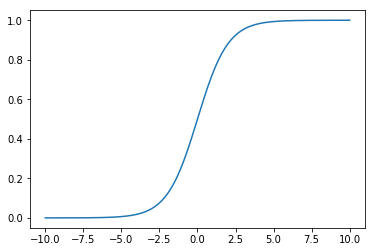
\includegraphics[scale=0.65]{img/funcion_logistica.png}
    \label{fig:logistica}
    \caption{Función Logística}
\end{figure}
La regresión logística es un método de regresión para el caso en que $Y_i \in \left \{0,1 \right \}$. El modelo considera: 

$$
p_i \equiv p_i(\beta) \equiv \mathbb{P}(Y_i=1 | X=x)= f(\beta_0+\sum_{j=1}^{k}\beta_{j} x_{ij}),
$$ 

con $f$ la función logística. De forma equivalente, si definimos $logit(p)=log(\dfrac{p}{1-p})$: 

$$
p_i=logit(p_i)= \beta_0+\sum_{j=1}^{k}\beta_j x_{ij}
$$

Como $Y_i$ son variables binarias, se tiene que   $Y_i|X_i=x_i \sim Ber(p_i)$. Así, la función de verosimilitud será:
$$
\mathcal{L}=\prod_{i=1}^{n} p_i(\beta)^{Y_i}(1-p_i(\beta))^{1-Y_i}
$$
Obtenemos el estimador de $\beta$, $\hat{\beta}$ usando método numéricos de optimización. 

\subsection{Sobre Regresión LinealEMV en práctica: tres ejemplos}
\label{sub:MV_tres_ejemplos}

\subsubsection{Regresión lineal y gaussiana} 
\label{sub:reg_lin}


Una aplicación muy popular del estimador de MV es en los modelos de regresión lineal y gaussianos. Consideremos el caso donde se desea modelar la cantidad de pasajeros que mensualmente viajan en una aerolínea, para esto, sabemos de nuestros colaboradores en la división de análisis de datos de la aerolínea que ésta cantidad tiene una tendencia de crecimiento cuadrática en el tiempo y además una componente oscilatoria de frecuencia anual. Estos fenómenos pueden ser explicados por el aumento de la población, los costos decrecientes de la aerolínea y la estacionalidad anual de las actividades económicas. 

Asumiendo que la naturaleza de la cantidad de pasajeros es estocástica, podemos usar los supuestos anteriores para modelar la densidad condicional  de dicha cantidad (con respecto al tiempo $t$) mediante una densidad normal parametrizada de acuerdo a 
\begin{equation}
	X \sim \cN\left(\theta_0 + \theta_1 t^2 + \theta_2\cos(2\pi t/12), \theta_3^2\right),
\end{equation}
donde $\theta_0,\theta_1,\theta_2$ parametrizan la media y $\theta_3$ la varianza. 

Consecuentemente, si nuestras observaciones están dadas por $\{(t_i,x_i)\}_{i=1}^n$ podemos escribir la log-verosimilitud de $\theta$ como 
\begin{align}
	\label{eq:logV_ejemplo_reg}
	l(\theta) 	&=\loga{\prod_{i=1}^n \frac{1}{\sqrt{2\pi\theta_3^2}}\expo{-\frac{(x_i-\theta_0 - \theta_1 t^2 - \theta_2\cos(2\pi t/12))^2}{2\theta_3^2}}}\nonumber \\
	&=\frac{n}{2}\loga{2\pi\theta_3^2}  - \frac{1}{2\theta_3^2}\sum_{i=1}^n (x_i - \theta_0 - \theta_1 t_i^2 - \theta_2\cos(2\pi t_i/12))^2
\end{align}
con lo que vemos que $\thetaMV$ puede ser calculado explícitamente y es función de $\{(t_i,x_i)\}_{i=1}^n$ debido a que la ecuación \eqref{eq:logV_ejemplo_reg} es cuadrática en $[\theta_0,\theta_1,	\theta_2]$.


% subsection estimador_de_mv_en_la_práctica_tres_ejemplos (end)

\subsubsection{Regresión no lineal: clasificación} 
\label{sub:clasif}

La razón por la cual $\thetaMV$ pudo ser calculado de forma explícita es porque el modelo Gaussiano con media parametrizada de forma lineal resulta en una log-verosimilitud cuadrática, donde el mínimo es único y explícito. Sin embargo, en muchas situaciones el modelo lineal y gaussiano no es el apropiado. 

Un ejemplo es esto es problema de evaluación crediticia (\textit{credit scoring}) donde en base a un conjunto de \textit{características} que definen a un cliente, un ejecutivo bancario debe evaluar si otorgarle o no el crédito que el cliente solicita. Para tomar esta decisión, el ejecutivo puede revisar la base de datos del banco e identificar los clientes que en el pasado pagaron o no pagaron sus créditos para determinar el perfil del \textit{pagador} y el del \textit{no-pagador}. Finalmente, un nuevo cliente puede ser \textit{clasificado} como pagador/no-pagador en base su similaridad con cada uno de estos grupos. 

Formalmente, denotemos las características del cliente como $t\in\R^N$ y asumamos que el cliente paga su crédito con probabilidad $\sigma(t)$ y no lo paga con probabilidad $1- \sigma(t)$, la función $\sigma(t)$ a definir. Esto es equivalente a construir la VA $X$
\begin{equation}
 	X|t \sim \ber{\sigma(t)}
 \end{equation} 
 donde $X=1$ quiere decir que el cliente paga su crédito y $X=0$ que no. Una elección usual para la función $\sigma(\cdot)$ es la función logística aplicada a una transformación lineal de $t$, es decir, 
 \begin{equation}
 	\Pr{(X=1|t)} = \frac{1}{1+e^{-(\theta_0 + \theta_1 t)	}}.
 \end{equation}
Notemos que este es un clasificador lineal, donde $\theta = [\theta_0, \theta_1]$ define un hiperplano en $\R^N$ en donde los clientes $t\in\{t | 0\leq \theta_0 + \theta_1 t\}$ pagan con probabilidad mayor o igual a 1/2 y el resto con probabilidad menor o igual a 1/2. Esto es conocido como \textbf{regresión logística}. 

Entonces, usando los registros bancarios $\{(x_i,t_i)\}_{i=1}^n$ ¿cuál es el $\theta = [\theta_0, \theta_1]$ de máxima verosimilitud? Para esto notemos que la log-verosimilitud puede ser escrita como 
\begin{align*}
	l(\theta) &= \log \prod_{i=1}^n p(x_i|t) \\
			  &= \sum_{i=1}^n x_i \log \sigma(t) + \left(n-\sum_{i=1}^n x_i\right)\log(1-\sigma(t))\\
			  &= \sum_{i=1}^n x_i \log \frac{1}{1+e^{-(\theta_0 + \theta_1 t)	}} + \left(n-\sum_{i=1}^n x_i\right)\log(1-\frac{1}{1+e^{-(\theta_0 + \theta_1 t)	}})
\end{align*}
Esta expresión no tiene mínimo global y a pesar que podemos calcular su gradiente, no podemos resolver $\partial l(\theta)/\partial \theta =0$ de forma analítica, por lo que debemos usar métodos de descenso de gradiente.  

\subsubsection{Variables latentes: \textit{Expectation-Maximisation}} 
\label{sub:EM}

En ciertos escenarios es natural asumir que nuestros datos provienen de una mezcla de modelos, por ejemplo, consideremos la distribución de estaturas en una población, podemos naturalmente modelar esto como una mezcla de distribuciones marginales para las estaturas de hombres y mujeres por separado, es decir, 
\begin{equation}
	X\sim p\cN(X|\mu_H,\Sigma_H) + (1-p)\cN(X|\mu_M,\Sigma_M)
\end{equation}
donde la verosimilitud de los parámetros $\theta = [p, \mu_H, \sigma_H,, \mu_M, \sigma_M]$ dado un conjunto de observaciones $\{x_i\}_{i=1}^n$ es
\begin{align*}
	L(\theta) 	&= \prod_{i=1}^n \left( p\cN(X|\mu_H,\Sigma_H) + (1-p)\cN(X|\mu_M,\Sigma_M) \right)\\
				&= \prod_{i=1}^n \left( p\frac{1}{\sqrt{2\pi\Sigma_H^{-1}}}\expo{\frac{-(x_i-\mu_H)^2}{2\Sigma^2_H}} + (1-p)\frac{1}{\sqrt{2\pi\Sigma_M^{-1}}}\expo{\frac{-(x_i-\mu_M)^2}{2\Sigma^2_M}}\right).
\end{align*}
Optimizar esta expresión con respecto a las 5 componentes de $\theta$ es difícil, en particular por la suma en la expresión, lo cual no permite simplificar la expresión mediante la aplicación de $\log(\cdot)$. 

Una interpretación de la diferencia de este modelo con respecto a los anteriores es la introducción implícita de una  \textit{variable latente} que describe de qué gaussiana fue generada cada observación. Si conociésemos esta variable latente, el problema sería dramáticamente más sencillo. En efecto, asumamos que tenemos a nuestra disposición las observaciones $\{z_i\}_{i=1}^n$ de la VA $\{Z_i\}_{i=1}^n$ las cuales denota de qué modelo es generada cada observación, por ejemplo, $Z_i=0$ (cf. $Z_i=1$) denota que el individuo con estatura $X_i$ es hombre (cf.~mujer).
 
En este caso, asumamos por un segundo que estas variables latentes están disponibles y consideremos los \textbf{datos completos} $\{(x_i,z_i)\}_{i=1}^n$ para escribir la función de verosimilitud completa mediante
\begin{align*}
	l(\theta|z_i,x_i) &= \prod_{i=1}^n \cN(X|\mu_H,\Sigma_H)^{z_i} \cN(X|\mu_M,\Sigma_M)^{(1-z_i)}\\
	&\hspace{-3em}= \sum_{i=1}^n \left( z_i\log\frac{1}{\sqrt{2\pi\Sigma_H^{-1}}}\expo{\frac{-(x_i-\mu_H)^2}{2\Sigma^2_H}} + (1-z_i)\log\frac{1}{\sqrt{2\pi\Sigma_M^{-1}}}\expo{\frac{-(x_i-\mu_M)^2}{2\Sigma^2_M}}\right).
\end{align*}
Esta función objetivo es mucho más fácil de optimizar, pero no es observable pues la VA $Z$ es desconocida. Una forma de resolver esto es tomando la esperanza condicional de la expresión anterior (con respecto a $Z$) condicional a los datos y los parámetros \textit{actuales}, para luego maximizar esta expresión c.r.a. $\theta$ y comenzar nuevamente. Específicamente, como la expresión anterior es lineal en $z_i$ basta con tomar su esperanza: 
\begin{align*}
	\Et{Z_i|\theta_t,x_i} &= 1\cdot\Prob{Z_i=1|\theta_t,x_i} + 0\cdot\Prob{Z_i=0|\theta_t,x_i}\\
	&= 	\frac{\Prob{x_i|\theta_t,z_i=1} p(z_i=1)}{p(x_i|\theta)}\\
	&= 	\frac{\Prob{x_i|\theta_t,z_i=1} p(z_i=1)}{p(x_i|z=1,\theta)p(z=1)+p(x_i|z=0	,\theta)p(z=0)}
\end{align*}

\section{Método de los Momentos}

Sean $X_1,...,X_n$ $n$ muestras i.i.d. de una variable aleatoria $X$ con función de densidad $p_X(x;\theta)$ o $f_X(x;\theta)$ en el caso de ser discreta o continua respectivamente, dependientes de un parámetro $\theta\in\mathbb{R}^k$ a estimar.

Recordar que los momentos de una variable aleatoria viene dado por $\mu_k=\mathbb{E}[X^k]$ donde $k$ representa el $k$-momento.

El estimador del método de los momentos es un estimador $\hat{\theta}\in\mathbb{R}^k$ de $\theta$ como la solución (si es que existe) de las $k$ ecuaciones simultaneas de los primeros $k$ momentos, esto es:

\begin{align*}
    \mathbb{E}[X^1]&=\dfrac{1}{n}\sum\limits_{i=1}^{n}x_i\\
    \mathbb{E}[X^2]&=\dfrac{1}{n}\sum\limits_{i=1}^{n}x_i^2\\
    \vdots\\
    \mathbb{E}[X^k]&=\dfrac{1}{n}\sum\limits_{i=1}^{n}x_i^k\\
\end{align*}

\begin{example}][Caso Exponencial]
Consideremos $X_1,...,X_n$ $n$ muestras i.i.d. de una variable aleatoria $X\sim exp(\theta)$ donde claramente $k=1$. Aplicando el método de los momentos, debemos resolver que:
\[\mathbb{E}[X]=\dfrac{1}{n}\sum\limits_{i=1}^{n}x_i\]

Por lo que 
\[\mathbb{E}[X]=\dfrac{1}{\theta}=\dfrac{1}{n}\sum\limits_{i=1}^{n}x_i\]

y entonces:

\[\hat{\theta}=\dfrac{1}{\dfrac{1}{n}\sum\limits_{i=1}^{n}x_i}\]

el cual calza justamente con el estimador EMV de $\theta$. 
\end{example}


\section{Intervalos de Confianza} 

En distintas situaciones, la estimación puntual de un parámetro puede no ser apropiada e incluso inverosímil, mientras que la distribución posterior puede ser poco interpretable por el público general. En dichos casos, es recomendable identificar un rango donde, con cierta probabilidad, el parámetro real está contenido. Esto motiva la siguiente definición: 

\begin{definition}[Intervalo de confianza]
\label{def:conf_inter} Un $(1-\alpha)$-intervalo de confianza para el parámetro $\theta$ fijo y desconocido, $\alpha\in[0,1]$, es el intervalo aleatorio $(A(X),B(X))$ tal que 
\begin{equation}
	\label{eq:conf_inter}
	\Probt{A(X)\leq\theta\leq B(X)} = 1-\alpha, \forall \theta\in\Theta.
\end{equation}
\end{definition}

\begin{remark}
	La definición del intervalo de confianza no describe una probabilidad sobre el parámetro $\theta$, pues estamos tomando un enfoque frecuentista (no bayesiano) donde éste es fijo. Por el contrario, lo que es aleatorio en la ecuación \eqref{eq:conf_inter} es el intervalo, no el parámetro. Entonces, si bien es una sutileza, la definición anterior se debe entender como la probabilidad de que ``el intervalo (aleatorio) contenga al parámetro (fijo)'', y no como la probabilidad de que ``el parámetro esté en el intervalo''. 
\end{remark}
Una consecuencia clave de este concepto es que si $I_{1-\alpha}$ es un $(1-\alpha)$-intervalo de confianza, entonces si fuese posible repetir una gran cantidad de veces el ejercicio de recolectar datos $X$ y calcular este intervalo para cada una de estas observaciones, entonces el parámetro $\theta$ estaría contenido en el intervalo un $100(1-\alpha)\%$ de las veces. Esto es muy diferente de asegurar que para un solo experimento, la probabilidad de que el parámetro $\theta$ esté contenido en $I_{1-\alpha}$ es $1-\alpha$, lo cual no es cierto. Los siguientes ejemplos tienen por objetivo ayudar a aclarar este concepto.

Para la construcción de intervalos de confianza es crucial la siguiente definición:

\begin{definition}[Pivote]

Sea $X=(X_1,...,X_n)$ una muestra aleatoria simple de una variable aleatoria cualquiera de depende de un parámetro $\theta$, el cual puede ser escalar o un vector. Sea $g(X,\theta)$ una variable aleatoria cuya distribución sea la misma para cualquier valor de $\theta$. A la función $g$ se de llama pivote.

\end{definition}

Veamos un ejemplo de la construcción de un pivote para el caso de la variable aleatoria normal.

\begin{example}[Intervalo de confianza para la media de la distribución normal]
	Consideremos la muestra $X_1,\ldots,X_n\sim\cN(\theta,1)$. Como $\bar{X}=\frac{1}{n}\sum_{i=1}^nX_i\sim\cN(\theta,1/n)$ tenemos que  
	\begin{equation}
			\sqrt{n}(\bar{X}-\theta)\sim\cN(0,1).
		\end{equation}	
	Esta cantidad es un \emph{pivote}. Consecuentemente, podemos identificar directamente un intervalo de confianza para el pivote desde una tabla de valores para la distribución normal de media cero y varianza unitaria. Si $\phi(x)$ denota la distribución Normal, entonces podemos elegir  $x_1$ y $x_2$ tal que $\phi(x_2)-\phi(x_1) = 1-\alpha$ con lo que tenemos
	\begin{equation}
	 	\Probt{x_1 \leq \sqrt{n}(\theta-\bar{X}) \leq x_2} = 1-\alpha \Leftrightarrow \Probt{\bar{X} + x_1/\sqrt{n} \leq \theta \leq \bar{X} + x_2/\sqrt{n}} = 1-\alpha,
	 \end{equation} 
	 es decir, $(\bar{X} + x_1/\sqrt{n},\bar{X} + x_2/\sqrt{n})$ es el $(1-\alpha)$-intervalo de confianza para $\theta$. 
	 
	 Eligiendo $\alpha=0.05$ una alternativa es tenemos $x_2 = -x_1 =1.96$, con lo que el intervalo de confianza del 95\% para $\theta$ está dado por 
	 \begin{equation}
	 	(\bar{X} -1.96/\sqrt{n},\bar{X} + 1.96/\sqrt{n}).
	 \end{equation}

	 El procedimiento estándar para encontrar intervalos de confianza es como el ilustrado en el ejemplo anterior, en donde construimos una cantidad que tiene una distribución que no depende del parámetro desconocido (llamada pivote). Construir un intervalo de confianza para esta cantidad es directo desde las tablas de distribuciones, luego, podemos encontrar el intervalo de confianza para la cantidad deseada, e.g., el parámetro desconocido, mediante transformaciones de la expresión del pivote. 

	 \begin{remark}
	 	El intervalo de confianza no es único. Por ejemplo, en el caso gaussiano podemos elegir en intervalo centrado en cero o desde $-\infty$. Esta elección dependerá de las aplicación en cuestión: una regla general es elegirlo de forma centrada para densidades que son simétricas, centrado en la moda para distribuciones unimodales, mientas que para densidades con soporte positivo podemos elegirlo desde cero. 
	 \end{remark}

	 Hasta ahora hemos solo definido intervalos de confianza para cantidades escalares, en donde el concepto de intervalo tiene sentido. Para parámetros vectoriales, nos referiremos a  \textit{conjuntos de confianza}. Siguiendo la Definición \ref{def:conf_inter}, un $(1-\alpha)$-conjunto de confianza $S(X)$ es tal que 
	 \begin{equation}
	\label{eq:conf_set}
	\Probt{\theta\in S(X)} = 1-\alpha, \forall \theta\in\Theta.
\end{equation}
\end{example}


\begin{exercise}
Considere $X_1,\ldots,X_{50}\sim\cN(0,\sigma^2)$, calcule el intervalo de confianza del 99\% para $\sigma$.
\end{exercise}

\begin{example}[Intervalo de confianza ---aproximado--- para Bernoulli] Consideremos $X_1,\ldots,X_{n}\sim\ber{\theta}$ y calculemos un intervalo de confianza para $\theta$. Recordemos que el EMV es $\thetahat = \frac{1}{n}\sum_{i=1}^nX_i$ y debido a la normalidad asintótica del EMV, tenemos que para $n$ grande, podemos asumir 
\begin{equation}
	\thetahat\sim\cN\left(\theta,\frac{\theta(1-\theta)}{n}\right),
\end{equation}
donde la varianza $\frac{\theta(1-\theta)}{n}=I_n(\theta)^{-1}$ es la inversa de la información de Fisher. 

Podemos entonces considerar el pivote
\begin{equation}
	\frac{\sqrt{n}(\thetahat-\theta)}{\sqrt{\theta(1-\theta)}}\sim\cN(0,1),
\end{equation}
y calcular el $(1-\alpha)$-intervalo de confianza asumiendo los valores $x_1$ y $x_2$ mediante 
\begin{align*}
	\Probt{x_1 \leq \tfrac{\sqrt{n}(\theta-\thetahat)}{\sqrt{\theta(1-\theta)}} \leq x_2} = 1-\alpha \Leftrightarrow \Probt{\thetahat + \tfrac{x_1\sqrt{\theta(1-\theta)}}{\sqrt{n}} \leq \theta \leq \thetahat + \tfrac{x_2\sqrt{\theta(1-\theta)}}{\sqrt{n}}} = 1-\alpha.
\end{align*}
Sin embargo, los bordes de este intervalo no son conocidos, pues dependen de $\theta$. Una forma de aproximar el intervalo es reemplazar el parámetro por su EMV. 
\end{example}


\begin{exercise}[Encuesta de elecciones presidenciales] Considere una encuesta que ha consultado a 1000 votantes y su candidato ha recibido 200 votos. Use el resultado del ejemplo anterior para determinar el intervalo de confianza del 95\% de la cantidad de votos que su candidato obtendría en la elección presidencial. 
\end{exercise}

Finalmente, revisaremos el siguiente ejemplo, el cual pretende ejemplificar el concepto de que en solo un experimento, la determinación del $(1-\alpha)$-intervalo de confianza no quiere decir que la probabilidad de que el parámetro esté contenido en él es $(1-\alpha)$\%. 

\begin{example}[Intervalo de confianza para una distribución uniforme]
\label{eq:unif_int_conf}Considere $X_1,X_2\sim\uni{\theta-\tfrac{1}{2},\theta+\tfrac{1}{2}}$ y observe que 
\begin{align*}
	\Probt{\min(X_1,X_2) \leq \theta \leq \max(X_1,X_2)} 
		&= \Probt{ X_1 \leq \theta \leq X_2}  + \Probt{ X_2 \leq \theta \leq X_1} \\
		&= \frac{1}{2}\times \frac{1}{2} + \frac{1}{2}\times\frac{1}{2}\\
		&= \frac{1}{2}
\end{align*}
corresponde al intervalo del 50\%. 

Sin embargo, si observáramos $X_1 = x_1$ y $X_2 = x_2$ tal que $|x_1-x_2|\geq\tfrac{1}{2}$ entonces necesariamente está contenido en el intervalo $(\min(X_1,X_2) , \max(X_1,X_2))$ con probabilidad 1. Esto ilustra la idea de que, en un experimento dado, la probabilidad de que $\theta$ esté en intervalo de confianza del $(1-\alpha)$\% no es necesariamente $(1-\alpha)$\%.
\end{example}


\section{Ejercicios}

\begin{enumerate}
    \item Se quiere estudiar el comportamiento de un vector bidimensional que tiene sus dos componentes ortogonales, independientes y que siguen una distribución normal. Al realizar las mediciones respectivas de cada componente, se obtiene una Muestra Aleatoria Simple (MAS, cada dato es generado desde una misma distribución y son independientes entre sí (iid)) $U=(U_1,...,U_n)$ de $n$ observaciones con $U_n\sim\mathcal{N}(0,\sigma^2)$  y una MAS $W=(W_1,...,W_n)$  de $n$ observaciones con $W_n\sim\mathcal{N}(0,\sigma^2)$. En específico, se busca estudiar el comportamiento de los módulos de los vectores obtenidos. Se obtiene una nueva MAS $X=(X_1,...,X_n)$ dada por:

\[X_i = \sqrt{U_i^2 - W_i^2}\]

\begin{enumerate}
    \item [i.] Encuentre la función de densidad de $X_1$\\
    \item Encuentre un estadístico suficiente para $\sigma^2$.
    \item Encuentre un estadístico suficiente minimal para $\sigma^2$.
    \item Encuentre el Estimador de Máxima Verosimilitud de $\sigma^2$.
    \item ¿Es el estimador $\widehat{\sigma^2}_{EMV}$ insesgado? Si no lo es, modifíquelo para que así sea.
    \item Encuentre un EIVUM de $\sigma^2$.
    \item Encuentre la distribución de  $\sqrt{n}(\widehat{\sigma^2}_{MLE}-\sigma^2)$
\end{enumerate}

\item Estudiaremos la varianza $\sigma^2$ de una Muestra Aleatoria Simple (MAS) $X=(X_1,...,X_n)$ donde $X_i\sim\mathcal{N}(\mu, \sigma^2)$, $\forall i =1,...,n$. Se considera que $\mu$ y $\sigma$ son parámetros desconocidos. 

Considere el siguiente estimador de la varianza dado por:

\[S^2 := \frac{1}{n-1}\sum\limits_{i=1}^{n}(\overline{X}_n-X_i)^2\]
donde $\overline{X}_n$ denota al promedio de $X_1,..., X_n$, es decir  $\overline{X}_n = \sum\limits_{i=1}^{n}X_i$. 
\begin{enumerate}
    \item [i.] Demuestre que $\mathbb{E}(S^2) = \sigma^2$ 
    \item [ii.] Calcule la varianza de $S^2$, para esto encontraremos primero la distribución de $\frac{n-1}{\sigma^2}S^2$, siga los siguientes pasos:
    \begin{enumerate}
        \item [ii.a.] Desarrolle la expresión $W=\sum\limits_{i=1}^{n}\frac{(X_i-\mu)^2}{\sigma^2}$ para llegar a:
        \[W = \frac{(n-1)}{\sigma^2}S^2  + \frac{n(\overline{X}_n-\mu)^2}{\sigma^2} \]
        \item [ii.b.] Encuentre las distribuciones asociadas a W y a $\frac{n(\overline{X}_n-\mu)^2}{\sigma^2} $
        \item [ii.c.] Aplique la función generadora de momentos en ambos lados de la ecuación. Para esto, asuma que $S^2$ es independiente de $\overline{X}_n$.
        \item [ii.d.] Encuentre la distribución de $\frac{n-1}{\sigma^2}S^2$
        \item [ii.e.] Calcule $\mathbb{V}(S^2)$
    \end{enumerate}
    \item [iii.] (Ejercicio) Calcule la varianza de $S^2$ desarrollando \textit{a mano} (Muy largo). 
\end{enumerate}


Ahora se considera otro estimador de la varianza dado por:

\[\hat{\sigma}^2 := \frac{1}{n}\sum\limits_{i=1}^{n}(\overline{X}_n - X_i)^2    \]

\begin{enumerate}
    \item [iv.] Muestre que $\hat{\sigma}^2$ cumple que $\mathbb{E}(\hat{\sigma}^2) \neq \sigma^2$ 
    \item [v.] Muestre que $\hat{\sigma}^2$ cumple que $\lim\limits_{n\rightarrow \infty} \mathbb{E}(\hat{\sigma}^2) = \sigma^2$
\end{enumerate}

\begin{enumerate}
    \item [vi.] Calcule $ECM_{\sigma^2}(S^2)$
    \item [vii.] Calcule $ECM_{\sigma^2}(\hat{\sigma}^2) $
    \item [viii.] Verifique que $ECM_{\sigma^2}(\hat{\sigma}^2) < ECM_{\sigma^2}(S^2)$
\end{enumerate}

\item \item Sea $X=(X_1,...,X_n)$ una MAS con una función de densidad dada por:
    \begin{equation}
        \nonumber 
        f(x|\theta)=\theta x^{\theta -1},\theta>0,x\in (0,1)
    \end{equation}
    \begin{itemize}
        \item Encuentre el estimador MLE para $\theta$. Calcule su esperanza y su varianza. ¿Cómo se comporta la varianza asintoticamente?
    
    \item[(vii)] ¿Es $\hat{\theta}_{MLE}$ insesgado para $\theta$? Si no lo es, modifíquelo con tal de que sea insesgado.
    
    \item[(viii)] Calcule el ECM de $\hat{\theta}_{MLE}$ y del estimador encontrado en la parte anterior. Basado en el criterio ECM, ¿Cúal de los dos estimadores es preferible?
    
    \item[(iX)] Denotemos como $\theta^{\star}$ al estimador encontrado en la parte (vii). ¿$\theta^{\star}$ alcanza la Cota de Cramer-Rao?
    
    \item[(X)] Si el estimador $\theta^{\star}$ no alcanza la Cota de Cramer Rao, ¿Tenemos que buscar un mejor estimador insesgado para $\theta$?
    \end{itemize}
    
    \item Sea $X=(X_1,...,X_n)$ una MAS con una función de densidad dada por:
\begin{equation}
    \nonumber 
    f(x|\theta)=\frac{2x}{\theta^2},\theta>0,0<x\leq \theta
\end{equation}

\begin{itemize}
    \item[(i)] Encuentre un estadístico suficiente para $\theta$.
    
    \item[(ii)] Encuentre un estadístico minimal suficiente para $\theta$.
    
    \item[(iii)] Encuentre el estimador MLE para $\theta$
    
    \item[(iv)] Calcule el ECM de $\hat{\theta}_{MLE}$
    
    \item[(v)] Si $\hat{\theta}_{MLE}$ es sesgado, modifíquelo para que sea insesgado. Denotémoslo como $\theta^{\star}$
    
    \item[(vi)] ¿Es $\theta^{\star}$ el mejor estimador insesgado de $\theta$?
\end{itemize}

\item Estudios relacionados con el comportamiento de ciertos bichos indican que estos tienden a organizarse al azar, linealmente, en un intervalo de longitud $\theta > 0$, a la derecha de un punto donde se ubica una feromona. Nos gustaría estimar el valor del parámetro $\theta$. Sea $X=(X_1,...,X_n)$ una muestra aleatoria simple (MAS) de la distancia de n bichos con respecto a la feromona.

\begin{enumerate}
    \item Defina el modelo paramétrico correspondiente.
    \item Considere el estimador $\hat{\theta}=2\Bar{X_n}$. ¿Será insesgado? Si no lo es, modifíquelo para que lo sea.
    \item Ahora, considere el estimador $\hat{\theta}=\max\{ X_1,...,X_n\}$. ¿Será insesgado? Si no lo es, modifíquelo para que lo sea.
    \item Calcule el ECM para cada uno de los estimadores y compárelos.
\end{enumerate}

\item
Considere un modelo lineal dado por $y_i=\beta x_i +\epsilon_i$ con $i=1,...,n$. Se tiene que $\epsilon_i$ son i.i.d. con $\mathbb{V}(\epsilon_i))=\sigma^2$, $\mathbb{E}(\epsilon_i)=0$ y que $X_i\perp \epsilon_i$, $\forall i$. Para estimar $\beta$ se han sugerido los siguientes estimadores:

\[\hat{\beta_1}=\frac{\sum\limits_{i=1}^{n}y_i}{\sum\limits_{i=1}^{n}x_i} \qquad\hat{\beta_2}=\frac{\sum\limits_{i=1}^{n}x_i y_i}{\sum\limits_{i=1}^{n}x_i} \]
Estudie el sesgo de cada estimador. Calcule la varianza de cada uno de los estimadores y compárelos con la varianza del estimador de MCO.

\item Considere el modelo lineal en forma matricial dado por:
\[Y=X\beta +\epsilon\]
Con $\beta\in\mathbb{R}^k$, $\mathbb{E}(\epsilon)=0_{nx1}$ y $\mathbb{V}(\epsilon)=\sigma^2Id_{n}$, con $\sigma$ un parámetro desconocido. Pruebe las siguientes propiedades del modelo:

\begin{itemize}
    \item $X^t\epsilon=0$
    \item $Y^tY=\hat{Y}^t\hat{Y}+\hat{\epsilon}^t\hat{\epsilon}$
    \item $\hat{\epsilon}^t\hat{\epsilon}=Y^tY-\hat{\beta}X^tY$
\end{itemize}

\item \textbf{Un poco de Geometría}
Llamemos $E_X$ al espacio generado por las columnas de X. Llamemos $P_X$ a la matriz que proyecta a un vector de $\mathbb{R}^n$ en el espacio generado por las columnas de X. Llamemos $E_{X^{\perp}}$ al espacio ortogonal a $E_X$. Se puede demostrar que la matriz que proyecta en el espacio generado por las columnas de X y la proyección en el ortogonal vienen dadas por:

\[P_X=X(X^tX)^{-1}X^t  \qquad P_{X^{\perp}}=Id- X(X^tX)^{-1}X^t  \]
Escriba los siguientes en términos de $P_X$ y $P_{X^{\perp}}$
\begin{itemize}
    \item $\hat{\epsilon}=Y-X\hat{\beta}$
    \item $\hat{Y}=P_X Y$
\end{itemize}
Se postula el siguiente estimador para la varianza de los errores $\sigma^2_\epsilon$:
\[\hat{\sigma_\epsilon^2}=\hat{\epsilon}^t\hat{\epsilon}\]
Escriba el estimador en términos de $P_X$ y $P_{X^{\perp}}$ y estudie su sesgo.
\end{enumerate}


\clearpage

\input{capitulos/Test de Hipótesis}\clearpage

\chapter{Enfoque bayesiano}

En esta sección complementaremos el enfoque visto hasta ahora en cuanto a la incorporación de un modelo para la incertidumbre asociada al parámetro $\theta$. En el paradigma bayesiano, consideraremos que el parámetro es una variable aleatoria, es decir, $\Theta$, la cual para una realización particular tomar el valor $\Theta = \theta$. Esto nos permite información \emph{a priori} sobre la estimación a realizar, lo que permite, en muchos casos, ayudar a la inferencia. Una diferencia conceptual entre ambos enfoques, es que la estadística frecuentista evita la subjetividad, mientras que la estadística bayesiana se basa en la convicción del(a) investigador(a), para emitir juicios sobre una hipótesis.

En este capítulo, se estudiará la estadística bayesiana y se introducirán los mismos conceptos vistos anteriormente desde el punto de vista bayesiano.




\section{Contexto y definiciones principales}

\begin{definition}[Distribución a priori]
La información, sesgos y cualquier otra característica conocida de $\Theta$ codificadas mediante la propia ley de probabilidad de esta VA, la cual tiene densidad $p(\theta)$, nos referimos a esta como la \emph{densidad a priori} o simplemente \emph{prior}.
\end{definition}

Con esta definición, podemos ver que la densidad conjunta de las VAs $X,\Theta$ pueden ser expresadas combinando la densidad a priori con el modelo visto en las secciones anteriores, es decir, 
\begin{equation}
    p(x,\theta) = p(x|\theta)p(\theta)
    \label{eq:joint_bayes}
\end{equation}
donde hemos escrito $p(x|\theta)$ en vez de $p_\theta(x)$ para hacer explícito que ahora consideramos el parámetro como una variable aleatoria. 

Adicionalmente, con la distribución conjunta en la ecuación \eqref{eq:joint_bayes}, podemos definir:

\begin{definition}[Distribución marginal]
La distribución de $X$, obtenida mediante la desintegración de parámetro $\Theta$ del par $(X,\Theta)$, es decir 
\begin{equation}
    p(x) = \int_\Omega p(x|\theta)p(\theta)\d\theta
\end{equation}
es conocida como distribución marginal de $X$.
\end{definition}

Consideremos ahora que tenemos un conjunto de observaciones denotado por $\mathcal{D}$, de un modelo estadístico con parámetro $\Theta$, entonces podemos definir

\begin{definition}[Función de verosimilitud]
La densidad de probabilidad evaluada en un conjunto de observaciones $\cD$ como función del valor del parámetro $\Theta$, es decir 
\begin{align}
    L: \Omega &\rightarrow \R\\
    \theta&\mapsto l(\theta) = L_\cD(\theta) = p(\cD|\theta),
\end{align}
recibe el nombre de función de verosimilitud, o en inglés, \emph{likelihood}. 
\label{función_verosimilitud}
\end{definition}
\begin{remark}
La función de verosimilitud no es una densidad de probabilidad, es decir, no es cierto que
\begin{equation}
    \int_\Omega L(\theta)\d\theta = 1
\end{equation}
\end{remark}

\begin{remark}
Dado que la función función de verosimilitud usualmente adquiere una forma exponencial (como por ejemplo en el caso de la familia exponencial), hay ocasiones en donde es conveniente usar la \emph{log-verosmilitud}, esto es, 
\begin{equation}
l(\theta)=\log L(\theta)=\log p(\cD|\theta).
\end{equation}
Esta formulación será particularmente útil cuando queramos optimizar la verosimilitud. 
\end{remark}

\begin{remark}
En general (pero no siempre) asumimos observaciones $\cD = {X_1,\ldots,X_n}$, $X_i\sim p(x|\theta)$, que son i.i.d. En cuyo caso, la verosimilitud factoriza de la forma $L_\cD(\theta) = \prod_{i=1}^n L_{X_i}(\theta)$, con lo cual la log-verosimilitud toma la forma: 
\begin{equation}
l_\cD(\theta) = \sum_{i=1}^nl_{X_i}(\theta)
\end{equation}
\end{remark}

\begin{example}
Considere los datos $\cD = \{x_1,...,x_n\}$, donde $x_i$ es la observación de una VA $X_i\sim \mathcal{N}(\mu,\sigma^2)$ iid con $\sigma^2$ conocido. La función  de verosimilitud de $\mu$ está dada por:

\begin{align}
L(\mu)=p(\cD|\mu)&=\prod_{i=1}^{n} \frac{1}{\sqrt{2 \pi \sigma^{2}}} 
\exp\left(\frac{-1}{2\sigma^{2}}(x_i-\mu)^{2}\right)\nonumber\\
&= \left(\frac{1}{\sqrt{2 \pi \sigma^{2}}}\right)^{n} \exp\left(\frac{-1}{2 \sigma^{2}} \sum_{i=1}^{n} (x_i - \mu )^{2}\right).
\end{align}

Luego, la log-verosimilitud está dada por:
\begin{equation}
    l(\mu)= \log L(\mu) = -\frac{n}{2} \log(2 \pi \sigma^{2}) + \frac{-1}{2\sigma^{2}} \sum_{i=1}^{n} (x_i - \mu )^{2}.
\end{equation}

\end{example}

Ahora estamos en condiciones de definir el elemento central de la inferencia bayesiana, sobre el cual todo el proceso de inferencia toma lugar. 

\begin{definition}[Distribución posterior]
\label{dist_posterior}
Dado el conjunto de observación $\cD$ la distribución \emph{posterior} del parámetro, es decir, considerando la inforamción reportada por los datos $\cD$, está dada por el teorema de Bayes mediante
\begin{align}
    p(\theta|\cD) = \frac{p(\cD)|\theta)p(\theta)}{p(\cD)}  \propto p(\mathcal{D}|\theta) p(\theta) \label{eq:posterior_def}
\end{align}

donde: 
\begin{itemize}
    \item $p(\theta)$ es el prior del parámetro.
    \item $p(\theta|\mathcal{D})$ es la posterior del parámetro. 
    \item $p(\mathcal{D}|\theta)$ es la verosimilitud
    \item $p(\mathcal{D}) = \int\Omega p(\mathcal{D}|\theta)p(\theta)\d \theta $ es la densidad marginal de los datos 
\end{itemize}
\end{definition}

La \emph{transición} de prior a posterior puede ser interpretada como el proceso de incorporar la evidencia de los datos (a través de la función de verosimilitud) para reducir la incertidumbre con respecto del valor del parámetro $\Theta$. De la ecuación \eqref{eq:posterior_def} podemos ver que este proceso, a veces referido como \emph{actualización bayesiana}, equivale a multiplicar por la verosimilitud, para luego normalizar, garantizando que $p(\theta|\cD)$ es en efecto una densidad de probabilidad. 

\begin{remark}
El símbolo $\propto$ en la ecuación \eqref{eq:posterior_def} es usado para indicar que el lado izquierdo es igual al lado derecho salvo una constante de proporcionalidad que depende de $\mathcal{D}$ y no de $\theta$. Con esto, cuando estemos calculando la posterior, solo nos enfocaremos en \emph{una versión proporcional}, pues luego la densidad posterior se puede encontrar mediante la normalización de esta última.
\end{remark}

\begin{example}[Posterior modelo Bernoulli]
\label{ej_post_bernoulli_1}
Sea $\theta$ la probabilidad de obtener cara al lanzar una moneda, y sean $X_1,..X_n$ $n$ resultados obtenidos al lanzar la moneda. Si no sabemos nada de $\theta$ antes del experimento, hace sentido tomar su prior como una distribución que de igual probabilidad a todo espacio de parámetros, es decir: $\theta \sim Unif(0,1)$. Notemos que el prior encapsula la infromación que tenemos antes del experimento. Modelamos $X_1,..X_n \sim Bernoulli(\theta)$. Entonces: 
$$
p(X_1,..X_n|\theta)=\prod_{i=1}^{n} \theta^{X_i} (1-\theta)^{1-X_i} = 
\theta^{\sum_{i=1}^{n} X_i} (1-\theta)^{n-\sum_{i=1}^{n}X_i}
$$
Notemos que en este caso, podemos calcular la distribución $p(X_1,..,X_n)$:
$$
p(X_1,..,X_n)=\int_{0}^{1} \theta^{\sum_{i=1}^{n} X_i} (1-\theta)^{n-\sum_{i=1}^{n}X_i} d\theta = B\left(\sum_{i=1}^{n} X_i +1 , n- \sum_{i=1}^{n} X_i +1 \right),
$$
donde $B(x,y)$ es la función beta:
$$
B(x,y)=\dfrac{\Gamma(x)\Gamma(y)}{\Gamma(x+y)}.
$$
Sea $s= \sum_{i=1}^{n}X_i$. Entonces la distribución a posteriori será:

$$
p(\theta|X_1,..X_n)= \dfrac{p(X_1,..X_n|\theta)}{p(X_1,..,X_n)} = \dfrac{1}{B(s+1,n-s+1)} \theta^{s} (1-\theta)^{n-s}.
$$

\end{example} 

Usualmente, es experimentos reales, los datos  $x_1,...,x_n$ son recibidos de forma secuencial, es decir, \emph{en línea}. De esta forma, es relevante notar que en primer lugar se observa $x_1$ primero, luego $x_2$, y así sucesivamente. \\

Consecuentemente, si se asume el prior para el parámetro $\theta$ dado por $p(\theta)$, es posible hacer la actualización bayesiana \emph{en línea} (o de forma adaptativa o continual), lo cual implica una corrección del modelo cada vez que se observan más datos. \\
Luego de observar $x_1$, la posterior $p(\theta|x_1)$ puede ser calculada como: 
$$
p(\theta|x_1) \propto p(x_1|\theta) p(\theta).
$$

Luego, al observar $x_2$, usamos el hecho que $X_1$ y $X_2$ son condicionalmente independientes dado $\theta$ y obtenemos: 
$$
p(\theta | x_1,x_2) \propto 
p(x_2|\theta) p(\theta|x_1) \propto p(x_1 |\theta) p(x_2|\theta) p(\theta) . 
$$
Con lo que para el caso general tenemos que 
$$
p(\theta | x_1,..x_n) \propto p(x_n|\theta) p(\theta|x_1,..x_{n-1}) \propto p(\theta) \prod_{i=1}^n p(\theta | x_i).
$$

\begin{remark}
Cuando las observaciones $\cD$ son condicionalmente independientes dado el parámetro $\theta$, entonces, la posterior $p(\theta|\cD)$ factoriza en las verosimilitudes de cada uno de los datos. 
\end{remark}

\begin{remark}
En la actualización bayesiana en línea, la posterior de la etapa $n$ sirve de prior de la etapa $n+1$.
\end{remark}


\section{Priors Conjugados}

La actualización bayesiana puede resultar en una posterior solo conocida de forma proporcional (cuando no es posible calcular la distribución marginal $p(x)$) o bien en una distribución que no pertenece a una familia conocida. Una herramienta que asegurar el cálculo de las distribuciones posteriores (incluyendo la constante de normalización) y que esta adopta una forma conocida es a través del uso de \textbf{priors conjugados}.
\begin{definition}

Sea un modelo con verosimilitud $p(x|\theta)$ y un prior sobre $\theta$ con densidad $p(\theta)$. Decimos que $p(\theta)$ es conjugado con la verosimiltud $p(x|\theta)$ si la posterior 
\begin{equation}
	p(\theta|x) = \frac{p(x|\theta)p(\theta)}{p(x)}
\end{equation}
pertenece a la\textit{misma familia} que el prior $p(\theta)$. Donde pertenecer a la misma familia quiere decir que ambas tienen una densidad de probabilidad definida por la misma forma funcional, e.g., $f_\lambda(\theta)$ pero con distintos valores para el \textit{parámetro} $\lambda$, el cual es un \textit{hiperparámetro} del modelo.
\end{definition}


\begin{example}[continuación de Ejemplo \ref{ej_post_bernoulli_1}]
\label{ej_post_bernoulli_2}
Tarea: Verifique si el Ejemplo \ref{ej_post_bernoulli_1} es en efecto uno de prior conjugado. 
\end{example}

\begin{example}[Distribución Multinomial]
Consideremos una variable aleatoria multinomial $X\sim\mul{n,\theta}$ donde $\theta$ pertenece al simplex 
\begin{equation}
	\label{eq:simplex}
  \{\theta\in[0,1]^k:\theta_1 + \cdots + \theta_k = 1 \}.
 \end{equation} 
 La distribución multinomial genera vectores $X\in\N^k$ cuya $i-$ésima componente modela la cantidad de veces que ocurre el evento $i$ dentro de $k$ eventos en $n$ intentos. Por ejemplo, si lanzamos un dado balanceado 100 veces, el vector que contiene el conteo de veces que obtenemos cada cara puede modelarse como 
 \begin{equation}
  	\theta_\text{dado} \sim \mul{100,\left[\tfrac{1}{6},\tfrac{1}{6},\tfrac{1}{6},\tfrac{1}{6},\tfrac{1}{6},\tfrac{1}{6}\right]}.
  \end{equation} 
Denotando $X=[x_1,\ldots,x_n]$, observemos que una muestra multinomial $X\sim\mul{n,\theta}$ cumple con 
\begin{equation}
	\{x_i\}_{i=1}^k \subset \{0,1,\ldots,n\},\quad  \sum_{i=1}^kx_i = n.
\end{equation}

Finalmente, la distribución Multinomial está dada por 
\begin{equation}
 	\mul{X;n,\theta} = \frac{n!}{x_1!\cdots x_k!} \theta_1^{x_1}\cdots\theta_k^{x_k},
 \end{equation} 
 y es la generalización de las distribuciones: 
\begin{itemize}
	\item Bernoulli cuando $k=2$ y $n=1$; pues $\ber{X;\theta} = \theta^{x} (1-\theta)^{1-x}$
	\item Categórica (o \emph{multinoulli}): cuando $n=1$; pues $\cat{X;\theta} = \theta_1^{x_1}\cdots\theta_k^{x_k}$
	\item Binomial: cuando $k=2$; pues $\bin{X;n,\theta} = \binom{n}{x} \theta^{x}(1-\theta)^{n-x}$
\end{itemize}
\end{example}

Observemos que el parámetro $\theta$ en la distribución multinomial (y las otras tres) es precisamente una distribución de probabilidad (discreta). Es decir, el construir un prior $p(\theta)$ implica definir una distribución sobre distribuciones discretas.  


\begin{definition}[Distribución de Dirichlet]
Consideremos la  distribución de Dirichlet
\begin{equation}
	\theta \sim \dir{\theta|\alpha} = \frac{1}{B(\alpha)} \prod_{i=1}^k \theta_i^{\alpha_i-1},
\end{equation}
donde $\alpha = (\alpha_1,\ldots,\alpha_k)$ es el parámetro de concentración y la constante de normalización está dada por $B(\alpha)=\prod_{i=1}^k\Gamma(\alpha_i)/\Gamma(\sum_{i=1}^k\alpha_i)$. El soporte de esta distribución es el simplex presentado en la ecuación \eqref{eq:simplex}.
\end{definition}


En el caso $k=3$, la distribución de Dirichlet puede ser graficada en el simplex de 2 dimensiones. La Figura \ref{fig:dist_Dirichlet} presenta tres gráficos para distintos valores del parámetro de concentración. 

\begin{figure}[H]
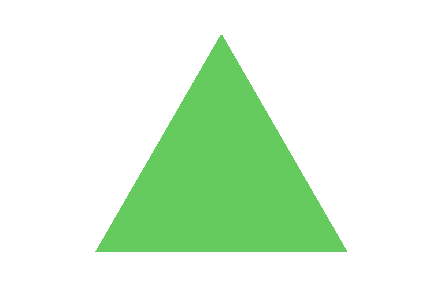
\includegraphics[width=0.3\textwidth]{img/dirichlet111.png}
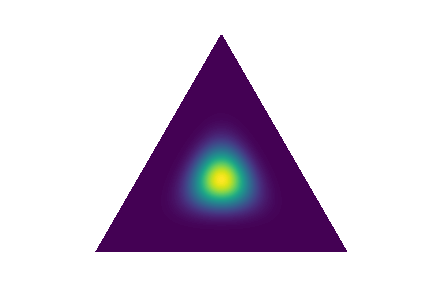
\includegraphics[width=0.3\textwidth]{img/dirichlet101010.png}
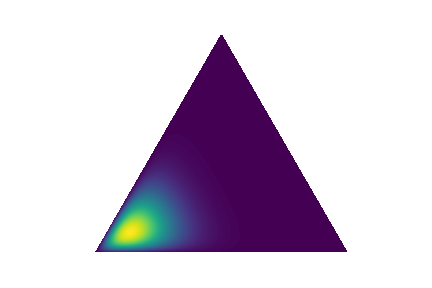
\includegraphics[width=0.3\textwidth]{img/dirichlet1022.png}
\caption{Distribuciones Dirichlet para $k=3$ con parámetros de concentración $\alpha$ (desde izquierda a derecha) dado por $[1,1,1]$, $[10,10,10]$ y $[10,2,2]$. }.
\label{fig:dist_Dirichlet}
\centering
\end{figure}


Veamos a continuación que la distribución de Dirichlet es conjugada al modelo Multinomial, y consecuentemente para Bernoulli, Categórica y Binomial. En efecto, si $\theta \sim \dir{\theta;\alpha}$ y $X\sim\mul{X;n,\theta}$, entonces

\begin{align}
	p(\theta|x) &= \frac{\mul{x;n,\theta}\dir{\theta;\alpha}}{p(x)}\nonumber\\
				&=  \frac{n!}{ x_1!\cdots x_k!p(x) B(\alpha)} \prod_{i=1}^k \theta_i^{x_i + \alpha_i-1}\nonumber\\
				&=  \frac{1}{B(\alpha')} \prod_{i=1}^k \theta_i^{\alpha'_i-1}
				\label{eq:dirichlet_post}
\end{align}
donde $\alpha' = (\alpha'_1,\ldots,\alpha'_k) = (\alpha'_1 + x_1,\ldots,\alpha'_k+ x_k)$ es el nuevo parámetro de concentración.

\begin{example}
	Consideremos $\alpha = [1,2,3,4,5]$ y generemos una muestra de $\theta\sim\dir{\theta|\alpha}$. El siguiente código genera, grafica e imprime esta muestra. 
	\begin{lstlisting}[language=Python]
	import numpy as np
	alpha = np.array([1,2,3,4,5]) 
	theta = np.random.dirichlet(alpha)
	plt.bar(np.arange(5)+1, theta);
	print(f'theta = {theta}')
\end{lstlisting}
En nuestro caso, obtuvimos los parámetros $ \theta = [0.034, 0.171, 0.286, 0.185, 0.324]$.

 Ahora, usaremos un prior Dirichlet sobre $\theta$ con $\alpha_p = [1,1,1,1,1]$ para calcular la posterior de acuerdo a la ecuación \eqref{eq:dirichlet_post}. La Figura \ref{fig:post_Dirichlet} muestra 50 muestras de la distribución posterior para distintas cantidades de observaciones entre 0 y  $ 10^5$. 

\begin{figure}[H]
\centering
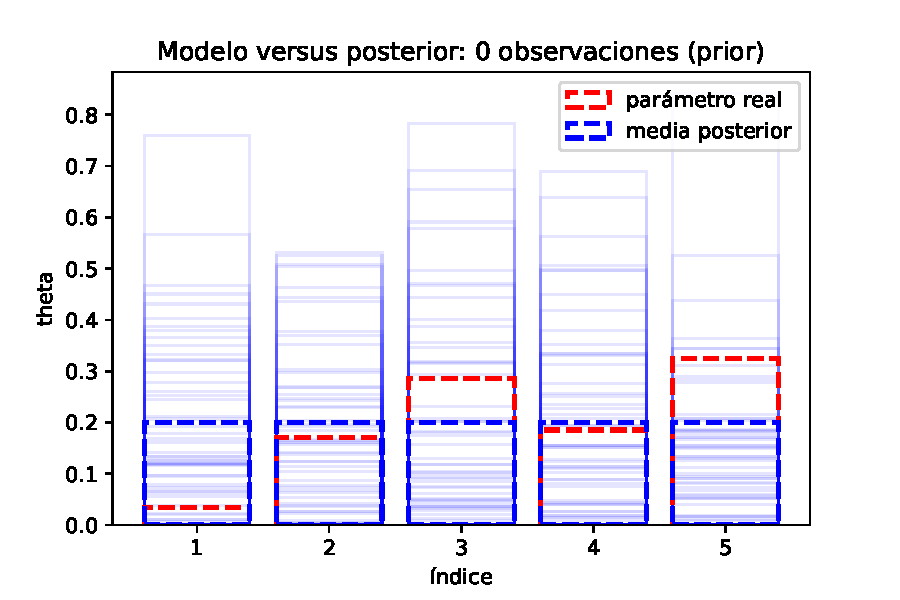
\includegraphics[width=0.3\textwidth]{img/post_dirichlet_0.pdf}
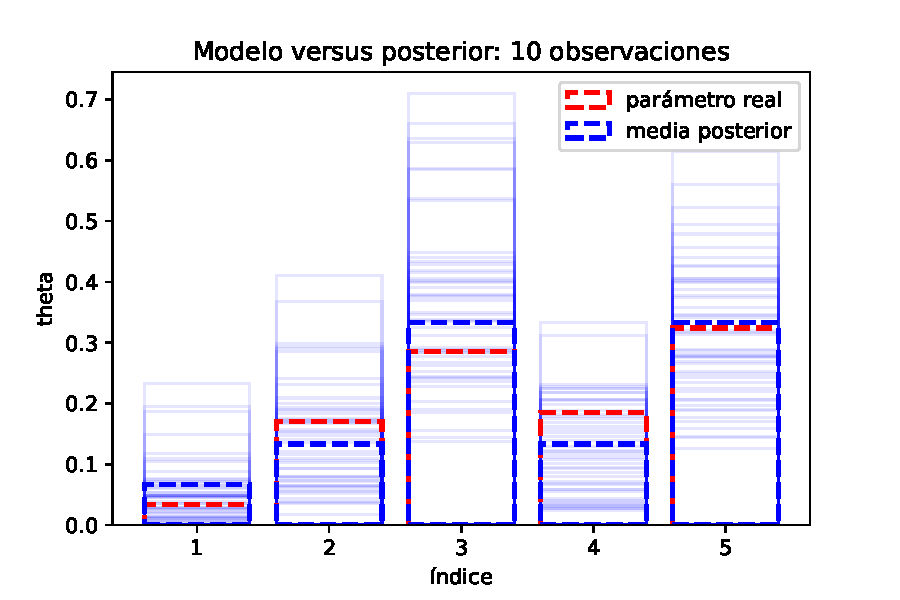
\includegraphics[width=0.3\textwidth]{img/post_dirichlet_10.pdf}
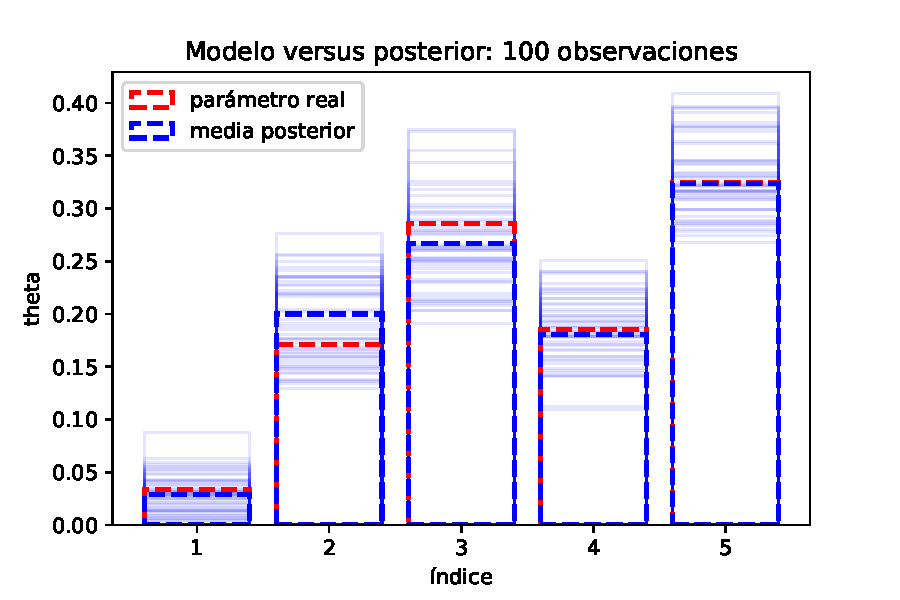
\includegraphics[width=0.3\textwidth]{img/post_dirichlet_100.pdf}\\
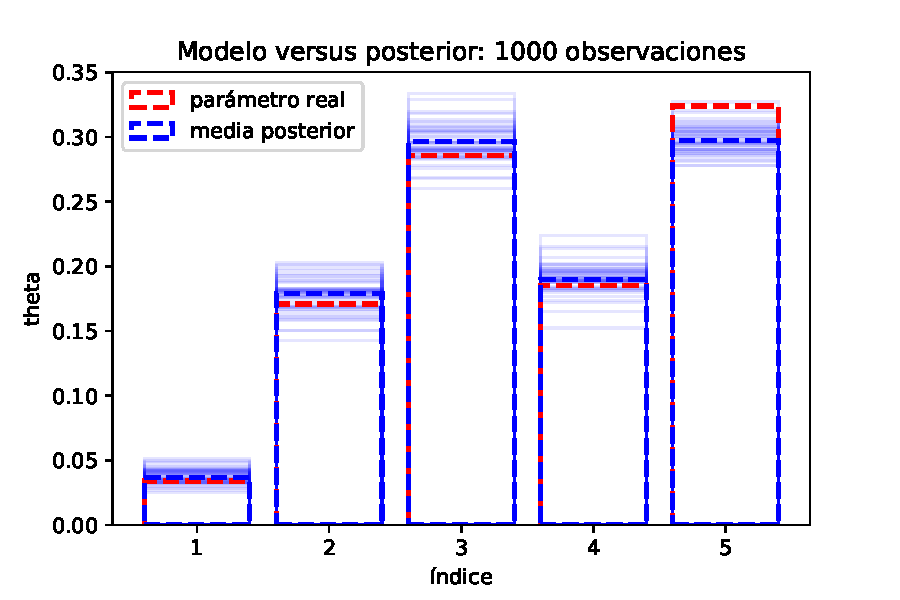
\includegraphics[width=0.3\textwidth]{img/post_dirichlet_1000.pdf}
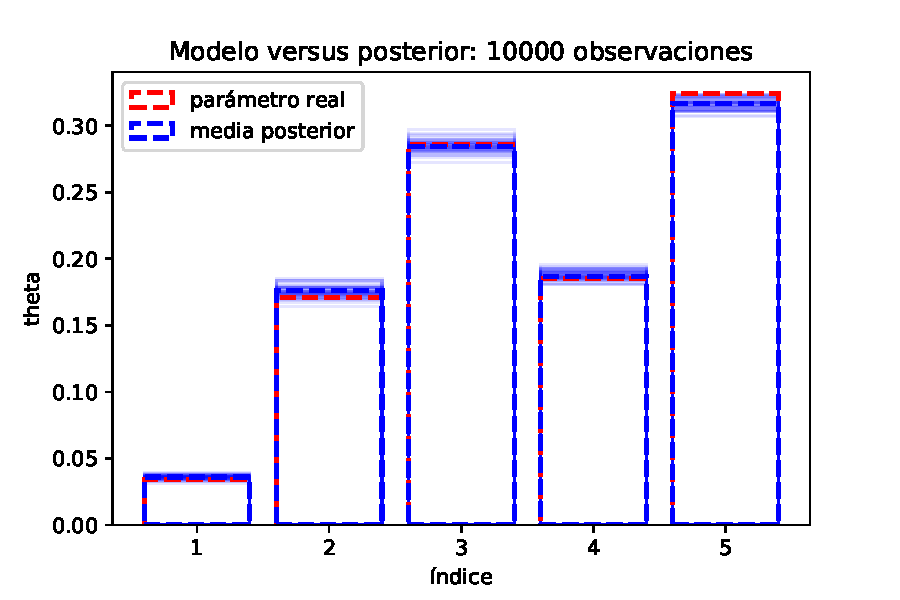
\includegraphics[width=0.3\textwidth]{img/post_dirichlet_10000.pdf}
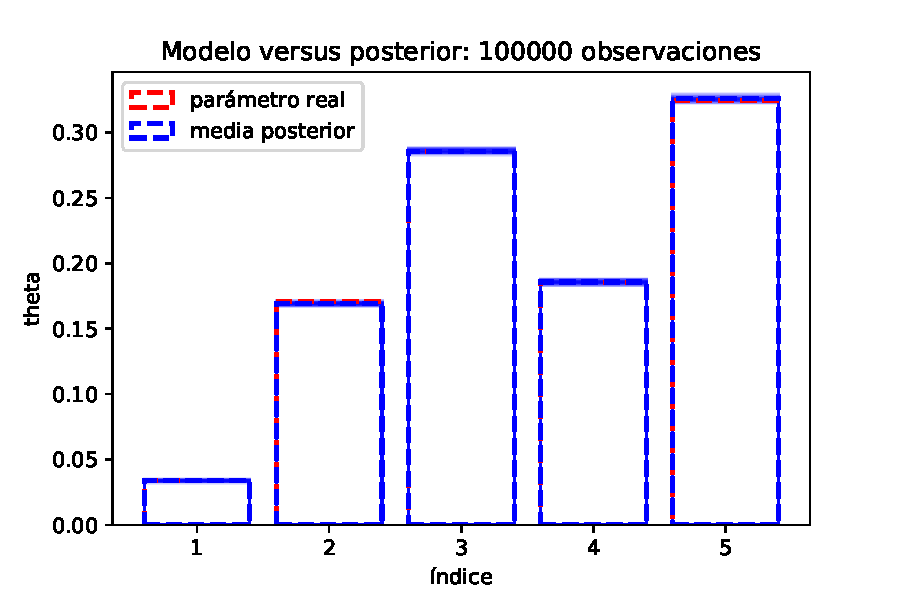
\includegraphics[width=0.3\textwidth]{img/post_dirichlet_100000.pdf}
\caption{Concentración de la distribución posterior en torno al parámetro real para un modelo $X\sim\mul{\theta}$ y una distribución a priori Dirichlet $\theta\sim\dir{\alpha}$. Se considera desde 0 hasta $10^5$ observaciones y cada gráfico (desde izquierda-arriba hasta derecha-abajo) muestra el parámetro real (linea roja quebrada), la media posterior (línea azul quebrada) y 50 muestras de la posterior (azul claro). Observe cómo la distribución a priori (línea azul quebrada en la primera figura) pierde importancia a medida que el número de observaciones aumenta.}
\label{fig:post_Dirichlet}
\end{figure}
\end{example}


\begin{example} \textbf{Modelo gaussiano ($\sigma^2$ conocido).} Consideremos el prior sobre la media $p(\mu) = \cN(\mu_0,\sigma_0^2)$, con lo que la posterior está dada por  
 \begin{align}
 	p(\mu|\mathcal{D}) &\propto \prod_{i=1}^n \frac{1}{\sqrt{2\pi\sigma^2}}\exp\left(-\frac{1}{2\sigma^2}(x_i-\mu)^2\right) \frac{1}{\sqrt{2\pi\sigma_0^2}}\exp\left(-\frac{1}{2\sigma_0^2}(\mu-\mu_0)^2\right)\label{eq:post_normal_mu_1}\\
 	&\propto \exp\left(-\frac{1}{2\sigma^2}\sum_{i=1}^n(x_i-\mu)^2-\frac{1}{2\sigma_0^2}(\mu-\mu_0)^2\right),\label{eq:post_normal_mu_2}
 \end{align} 
 donde la proporcionalidad viene de ignorar la constante $p(\mathcal{D})$ en la primera línea e ignorar todas las contantes que no dependen de $\mu$ en la segunda línea. Recordemos que estas constantes para $\mu$ incluyen a la varianza de $x$, $\sigma^2$, por lo que ignorar esta cantidad es solo posible debido a que estamos considerando el caso en que $\sigma^2$ es conocido. Completando la forma cuadrática para $\mu$ dentro de la exponencial en la ec.~\eqref{eq:post_normal_mu_2}, obtenemos
 \begin{equation}
 	p(\mu|\mathcal{D}) \propto \exp\left(-\frac{1}{2\sigma_n^2}(\mu - \mu_n)^2\right),\label{eq:post_normal_mu_3}
 \end{equation} 
 donde (ya definiremos $\mu_n$ y $\sigma_n^2$ en breve) como $p(\mu|\mathcal{D})$ debe integrar uno, la única densidad de probabilidad proporcional al lado derecho de la ecuación anterior es la Gaussiana de media $\mu_n$ y varianza $\sigma_n^2$. Es decir, la constante de proporcionalidad necesaria para la igualdad en la expresión anterior es
 \begin{equation}
     \int_\R\exp\left(-\frac{1}{2\sigma_n^2}(\mu - \mu_n)^2\right)\d\mu = (2\pi\sigma_n^2)^{n/2}.
 \end{equation} Consecuentemente, confirmamos que el prior elegido era efectivamente conjugado con la verosimilitud gaussiana, con lo que la posterior está dada por la siguiente densidad (gaussiana):
  \begin{equation}
 	p(\mu|\mathcal{D}) = \cN(\mu;\mu_n,\sigma_n^2) = \frac{1}{(2\pi\sigma_n^2)^{N/2}}\exp\left(-\frac{1}{2\sigma_n^2}(\mu - \mu_n)^2\right),\label{eq:post_normal_mu_4}
 \end{equation} 
 donde la media y la varianza están dadas respectivamente  por 
 \begin{align}
 	\mu_n &= \frac{1}{\tfrac{1}{\sigma_0^2} + \tfrac{n}{\sigma^2}} \left(\frac{1}{\sigma_0^2}\mu_0 + \frac{n}{\sigma^2}\bar{x} \right), \quad \text{donde } \bar{x} = \frac{1}{n}\sum_{i=1}^n x_i\label{eq:post_Gm}\\
 	\sigma_n &= \left(\frac{1}{\sigma_0^2} + \frac{n}{\sigma^2}\right)^{-1}.\label{eq:post_Gv}
 \end{align}
\end{example}
\begin{remark}
	La actualización bayesiana transforma los parámetros del prior de  $\mu$ desde  $\mu_0$ y $\sigma_0^2$ hacia $\mu_n$ y $\sigma_n^2$ en las ecs.~\eqref{eq:post_Gm} y \eqref{eq:post_Gv} respectivamente. Notemos que los  parámetros de la posterior son combinaciones (interpretables por lo demás) entre los parámetros del prior y los datos, en efecto, la $\mu_n$ es el promedio ponderado entre  $\mu_0$ (que es nuestro candidato para $\mu$ antes de ver datos) con factor $\sigma_0^{-2}$ y el promedio de los datos $\bar{x}$ con factor $(\sigma^{2}/n)^{-1}$, que a su vez es el estimador de máxima verosimilitud. Es importante también notar que  estos  factores son las varianzas inversas---i.e., precisión---de $\mu_0$ y de $\bar{x}$. Finalmente, observemos que $\sigma_n$ es la \emph{suma paralela} de las varianzas, pues  si expresamos la ec.~\eqref{eq:post_Gv} en términos de \emph{precisiones}, vemos que la precisión inicial $\sigma_0^2$ aumenta un término $\sigma^2$ con cada dato que vemos; lo cual tiene sentido pues con más información es la precisión la que debe aumentar y no la incertidumbre (en este caso representada por la varianza).
\end{remark}
\begin{example} \textbf{Modelo gaussiano ($\mu$ conocido).} Ahora procedemos con el siguiente prior para la varianza, llamado Gamma-inverso:
 \begin{equation}
 	p(\sigma^2)= \text{inv-}\Gamma(\sigma^2;\alpha,\beta) = \frac{\beta^\alpha}{\Gamma(\alpha) (\sigma^2)^{\alpha+1}}\exp(-\beta/\sigma^2)
 \end{equation}
 esta densidad recibe dicho nombre pues es equivalente a modelar la precisión, definida como el recíproco de la varianza $1/\sigma^2$, mediante la distribución Gamma. Los hiperparámetros $\alpha$ y $\beta$ son conocidos como parámetros de forma y de tasa (o precisión) respectivamente. 

 Con este prior, la posterior de la varianza toma la forma:
 \begin{align}
 	p(\sigma^2|\mathcal{D}) &\propto \prod_{i=1}^N \frac{1}{\sqrt{2\pi\sigma^2}}\exp\left(-\frac{1}{2\sigma^2}(x_i-\mu)^2\right) \frac{\beta^\alpha}{\Gamma(\alpha) (\sigma^2)^{\alpha+1}}\exp(-\beta/\sigma^2)\\
 	&\propto  \frac{1}{(\sigma^2)^{N/2+\alpha+1}}\exp\left(-\frac{1}{\sigma^2}\left(\frac{1}{2}\sum_{i=1}^N(x_i-\mu)^2 +\beta\right) \right)\nonumber
 \end{align} 
 donde nuevamente la proporcionalidad ha sido mantenida debido a la remoción de las constantes. Esta última expresión es proporcional a una distribución Gamma inversa con hiperparámetros $\alpha$ y $\beta$ ajustados en base a los datos observados. 


\end{example}




Hay ocasiones en las que el conocimiento a priori sobre el parámetro no puede ser convenientemente expresado mediante una densidad de probabilidad pero sí una densidad que no necesariamente integra uno o incluso es (Lebesgue) integrable. Para reflejar esta idea, se usan priors impropios.

\begin{definition}[Prior impropia] Una distribución a priori impropia es una distribución que no es necesariamente de probabilidad (i.e., no integra 1), pero que de todas formas puede ser utilizada como distribución a priori en el contexto de inferencia bayesiana, pues la distribución posterior correspondiente si es una distribución de probabilidad apropiada. 
\end{definition}

\begin{remark} No es necesario usar la constante de normalización en las densidades a priori Gaussianas (o ninguna otra en realidad).
\end{remark}

\begin{remark} Veamos que un prior impropio puede incluso tener integral infinita, en el caso de la distribución normal $X\sim\cN(X;\mu,1)$,  $\mu\in\R$, podemos elegir $p(\mu)\propto1$ y escribir 
\begin{equation}
	p(\mu|x)\propto p(x|\mu)\cdot 1 = \cN(x;\mu,1) = \cN(\mu;x,1). 
\end{equation}
	
\end{remark}

Considerar distribuciones uniformes impropias como priors no informativas parece tener sentido, pues intuitivamente no estamos dando preferencia (mayor probabilidad a priori) a ningún valor del parámetro por sobre otro. Sin embargo, este procedimiento sufre de una desventaja conceptual.




\section{Estimación y predicción}

\subsection{Estimadores bayesianos}

Si bien ya hemos estudiado el rol del prior en la inferencia bayesiana, hasta ahora no lo hemos considerado en la construcción de estimadores. En particular, el EMV no incorpora conocimiento a priori del parámetro. Con el objetivo de incorporar este conocimiento a priori en el cálculo de estimadores puntales, consideramos que en el caso general, podemos considerar otros estimadores puntuales a través de una función de pérdida asociada a estimar el parámetro $\theta$ mediante el estimador $\hat\theta$ dada por $L(\theta,\hat\theta)$. Con esto podemos definir los conceptos de riesgo y estimador bayesiano.

\begin{definition}[Riesgo bayesiano]
Para una función de pérdida $L(\theta,\hat\theta)$ y un conjunto de observaciones $\cD$, el riesgo bayesiano es la esperanza posterior de dicha función de pérdida, es decir
\begin{equation}
    R(\hat\theta) = \int_\Omega L(\theta,\hat\theta)p(\theta|\cD)\d\theta.
\end{equation}
\end{definition}



\begin{definition}[Estimador bayesiano]
Dado un conjunto de datos $\cD$ y un riesgo bayesiano $R(\theta)$, un estimador bayesiano es uno que minimiza el riesgo bayesiano:
\begin{equation}
    \theta_\text{Bayes}(\cD) = \arg\min_{\Omega} R(\theta).
\end{equation}
donde es implícito que $R(\cdot)$ se define con $\cD$.
\end{definition}

A continuación, se definirán estimadores bayesianos  con distintas funciones de costo o de riesgo.


\begin{definition}[Bayes' Least-Squares (BLS)]
El  caso estándar es la función de pérdida cuadrática $L_2(\theta,\hat\theta) = (\theta-\hat\theta)^2$ la cual resulta en el estimador dado por la media posterior $\theta_\text{Bayes}(\cD) = \E{\theta|\cD}$
\end{definition}


\begin{definition}[Minimum absolute-error (MAE)]

De forma similar,la función de costo $L_1(\theta,\hat\theta) = |\theta-\hat\theta|_1$ resulta en el estimador dado por la mediana posterior.
\end{definition}

Encontrar una función de pérdida para el máximo a posteriori es menos directo. Consideremos en primer lugar el caso $\theta\in\Omega$ discreto y la pérdida ``0-1''
\[   
L_\text{0-1}(\theta,\hat\theta) = 
     \begin{cases}
       0 &\quad\text{si } \theta = \hat\theta,\\
       1 &\quad\text{si no}. 
     \end{cases}
\]

El riesgo de Bayes asociado a $L_\text{0-1}(\theta,\hat\theta)$ (en el caso discreto) toma la forma
\begin{equation}
    R(\hat\theta) = \Prob{\theta\neq\hat\theta|\cD} = 1-\Prob{\theta = \hat\theta|\cD},
\end{equation}
lo cual es minimizado eligiendo $\hat\theta$ tal que $\Prob{\theta = \hat\theta|\cD}$ es máximo, es decir, el MAP. ¿por qué no es posible proceder de esta forma para el caso continuo? ¿cuál es la función de costo asociada al MAP en el caso continuo?

\begin{definition}[Estimador máximo a posteriori]
Sea $\theta \in \Theta$ un parámetro con distribución a posteriori $p(\theta |D)$ definida en todo $\Theta$. Entonces nos referiremos a su estimación puntual dada por: 
$$
\theta_{MAP}= \underset{\Theta}{\arg\max}\ p(\theta|D),
$$

como el estimador \emph{máximo a posteriori} (MAP). Se utiliza la siguiente función de costo:

\[C(a,b)=\begin{cases}
  1, &|a-b|>0\\
  0, \sim
\end{cases}\]
\end{definition}

\begin{remark}
Es posible encontrar el MAP solo teniendo acceso a una versión \emph{proporcional} a la distribución posterior, un escenario usual en inferencia bayesiana, o también mediante la maximización del logaritmo de ésta última. En efecto, 
$$
\theta_{MAP} = \underset{\theta \in \Theta}{\arg\max }\ p(\theta|\mathcal{D}) = \underset{\theta \in \Theta}{\arg\max }\ p(\mathcal{D}|\theta)p(\theta)= \underset{\theta \in \Theta}{\arg\max}\left(\underbrace{\log p(\mathcal{D}|\theta)}_{l(\theta)} + \log p(\theta)\right),
$$
donde hemos encontrado la maximización de  la función de log-verosimilitud, pero ahora junto al log-prior.
\end{remark}

\begin{remark}
Es relevante notar que el estimador MAP es una \emph{modificación} del EMV, pues ambos comparten una parte de la misma función objetivo (verosimilitud) con la diferencia que el MAP además incluye el término \emph{log-prior}. Esto puede entenderse como una regularización de la solución del problema de MV, en donde el término adicional puede representar las propiedades del estimador más allá de que las pueden ser exclusivamente revelada por los datos. 
\end{remark}

\begin{example}[Máximo a posterior para el modelo gaussiano]
En particular, para el modelo lineal y gaussiano que hemos considerado hasta ahora, podemos calcular $\theta_{MAP}$ para un prior Gaussiano de media cero y varianza $\sigma_\theta^2$. Éste está dado por (asumimos la varianza del ruido $\sigma_\epsilon^2$ conocida):	
\begin{align}
	\theta_\text{MAP}^\star 	&= \text{argmax } p(Y|\theta,X)p(\theta)\nonumber\\
	\text{[ind., def.]}\ &= \text{argmax } \prod_{i=1}^N \cN(y_i;\theta^\top x_i,\sigma_\epsilon^2)\cN(\theta;0,\sigma_\theta^2) \nonumber\\
	&= \text{argmax } \prod_{i=1}^N \frac{1}{\sqrt{2\pi}\sigma_\epsilon} \exp\left({\frac{-1}{2\sigma_\epsilon^2}(y_i-\theta^\top x_i)^2}\right)											\frac{1}{(\sqrt{2\pi}\sigma_\theta)^{M+1}} \exp\left({\frac{-||\theta||^2}{2\sigma_\theta^2}}\right) \nonumber\\
	 &= \text{argmax } \frac{1}{\sqrt{2\pi}\sigma_\epsilon} \frac{1}{(\sqrt{2\pi}\sigma_\theta)^{M+1}} \exp\left( \sum_{i=1}^N{\frac{-1}{2\sigma_\epsilon^2}(y_i-\theta^\top x_i)^2} -{\frac{||\theta||^2}{2\sigma_\theta^2}}\right) \nonumber\\
	\text{[log.]}\  &= \text{argmin } \sum_{i=1}^N{(y_i-\theta^\top x_i)^2} +{\frac{\sigma_\epsilon^2}{\sigma_\theta^2}||\theta |^2}.\nonumber 
	\label{eq:MAP_reg_lin}
\end{align}
Podemos ver que eligiendo un prior uniforme o de normal de varianza muy amplia, el MAP es equivalente al EMV. ¿qué significa esto? ¿qué comportamiento differente de EMV promueve el MAP en este caso?
\end{example}






\subsection{Posterior predictiva}

En la inferencia bayesiana las predicciones ocupan un rol relevante, pues luego de realizar inferencia sobre un modelo estadístico, en general estamos interesados estudiar cómo serán los siguientes datos genearados por el modelo. Para esto definiremos la predicción bayesiana de la forma

\begin{definition}[Posterior predictiva]
Para un conjunto de datos $\cD$ y un parámetro $\theta$, la densidad posterior predictiva está dada por
\begin{equation}
    p(x|\cD) = \int_\Omega p(x|\theta)p(\theta|\cD)\d\theta = \E{p(x|\theta) |\cD},
\end{equation}
es decir, el valor esperado del modelo estadístico con respecto a la ley posterior del parámetro (modelo).
\end{definition}
Podemos ahora considerar la posterior predictiva como nuestro modelo \emph{aprendido} y generar datos de él, donde nos encontramos frente al mismo dilema de un estimador puntual como en el caso anterior: es posible considerar muestras aleatorias, la media, la mediana o algún intervalo. 

\begin{remark}
La posterior predictiva es distinta (en general) a la predicción \emph{plug-in}, en donde consideramos en modelo estadístico $p_{\hat\theta}$ en base a un estimador (puntual) cualquiera $\hat\theta$. Desde esa perspectiva, la posterior predictiva equivale a considerar estimadores y modelos puntuales pero integrar todos ellos con respecto a la ley posterior. 
\end{remark}

\newpage


\section{El prior de Jeffreys}

Consideremos $X\sim p(x|\theta)$, $\theta \in [a,b]$, en donde elegimos el prior \textit{no informativo} uniforme dado por 
$$
	p(\theta) =\uni{a,b} = \frac{1}{b-a}.
$$
Consideremos ahora un modelo \textit{reparametrizado} $\eta = e^\theta\in[c,d]$, donde el modelo es expresado como $X\sim q(x|\eta) = p(x|\theta) $. El prior uniforme para el nuevo parámetro es
\begin{equation}
	p(\eta) =\uni{c,d} = \frac{1}{d-c}.
\end{equation}
Observemos que la elección uniforme del parámetro $\theta$ en el intervalo $[a,b]$ es equivalente a elegir $\eta$ según
\begin{equation}
	\tilde{p}(\eta) = p(\theta) \left|\frac{d\theta}{d\eta}\right| = \frac{1}{b-a}\left|\frac{d\log\eta}{d\eta}\right|= \frac{1}{\eta (b-a)},
\end{equation}
es decir, la distribución sobre $\eta$ inducida por $p(\theta)$. Esta distribución por supuesto no es equivalente a elegir $\eta$ uniformemente en el intervalo $[c,d]$. 

\begin{remark}
¿Es un prior uniforme realmente no informativo si luego de elegir otra parametrización este ya no es uniforme? ¿Es posible construir un prior no informativo?
\end{remark}

Una forma de construir un prior que es invariante ante reparametrizaciones es mediante la metodología propuesta por  Harold Jeffreys (1946), el que sugiere elegir un prior proporcional a la raíz cuadrada del determinante de la información de Fisher, es decir,  
\begin{equation}
	p(\theta) \propto \left( I(\theta)\right)^{1/2},
\end{equation}
donde recordemos que la información de Fisher está dada por 
\begin{equation}
	I(\theta) = -\Et{\frac{\partial^2}{\partial\theta^2}\log p(X|\theta)} = \Et{\left(\frac{\partial}{\partial\theta}\log p(X|\theta)\right)^2}.
\end{equation}
Además, si $X_1,\ldots,X_n$ son iid, entonces $I(\theta) = n I_1(\theta)$ y el prior de Jeffreys puede ser expresado como 
\begin{equation}
	p(\theta) \propto  I_1(\theta)^{1/2}.
\end{equation}
Observemos que si $\int_\Omega\sqrt{I(\theta)}\d\theta$ es finito, entonces la constante de proporcionalidad es precisamente esta cantidad. Sin embargo, si esta cantidad es infinita el prior de Jeffreys aún es un prior válido pero impropio, siempre y cuando las posteriores respectivas sí sean propias. 

Veamos ahora que el prior de Jeffreys es invariante bajo reparametrizaciones. Consideremos los modelos relacionados mediante reparametrización dados por 
\begin{equation}
	X\sim p(x|\theta),\ \theta\in\Omega\quad \& \quad X\sim q(x|\eta),\ \eta\in\Gamma,
\end{equation}
donde $\eta = h(\theta)$. Las informaciones de Fisher para ambos modelos, denotadas respectivamente $I_p(\theta)$ e $I_q(\theta)$, están relacionadas mediante
\begin{align}
	I_p(\theta) &= \int_\cX\left(\frac{\partial}{\partial\theta}\log p(x|\theta)\right)^2p(x|\theta)\d x\nonumber\\
				&= \int_\cX\left(\frac{\partial}{\partial\theta}\log q(x|h(\theta))\right)^2q(x|h(\theta))\d x\nonumber\\
				&= \int_\cX\left(\frac{\partial}{\partial\eta}\log q(x|\eta) h'(\theta)\right)^2q(x|\eta)\d x\nonumber\\
				&= \left(h'(\theta)\right)^2 I_q(\eta).
\end{align} 

Observemos ahora que el prior en $\theta$, $p(\theta)$, inducido por el prior de Jeffreys en $\eta$, $p_J(\eta)$, es efectivamente el prior de Jeffreys en $\theta$, $p_J(\theta)$. En efecto, debido al cambio de variable tenemos

\begin{equation}
	p(\theta) = p_J(\eta) \left|\frac{d \eta}{d \theta}\right| = \sqrt{I_q(\eta)}\left|h'(\theta)\right| = \sqrt{I_p(\theta)} = p_J(\theta).
\end{equation}

Como ya mencionamos, la construcción del Prior de Jeffreys surge con la idea de usar un prior que sea invariante bajo transformaciones monótonas y que sea no informativo. ¿Pero cómo se logra esto últmo? Resulta ser que el prior de Jeffreys es el prior uniforme sobre el espacio de parámetros $\Theta$, pero no con la métrica euclidiana. Intuitivamente, la topología que se debe considerar es aquella que calcula la distancia entre dos parámetros $\theta_1$ y $\theta_2$ como la divergencia de Kulback-Liebler entre sus distribuciones asociadas $f(x|\theta_1)$ y $f(x|\theta_2)$.

\section{Intervalos de Credibilidad}

En el concepto (frecuentista) de intervalo de confianza, la  \emph{aleatoriedad} ocurre antes que veamos los datos, pues recordemos que los supuestos de este paradigmas son que el parámetro es fijo y desconocido, y la generación de datos es aleatoria. Con esto, el hecho de encontrar un intervalo de confianza del, e.g., 95\% quiere decir que existe un 95\% de probabilidad de que un intervalo de confianza observado en el futuro (en realidad lo observado son los datos y el intervalo es función de éstos) contengan al parámetro. Esto es contraintuitivo, pues nos gustaría que la {aleatoriedad} ocurriera \emph{después de observar los datos}, es decir, dado los datos $x$ cual es la probabilidad de que el parámetro está dentro de un intervalo dado?

El paradigma bayesiano permite enunciar lo anterior y propone una noción de intervalos de confianza más natural que el enfoque frecuentista, pues para $ C_x\subset \Omega$, la expresión $\mathbb{P}(\theta \in)$ tiene un significado, incluso condicional a $x$. En este caso, le llamamos intervalos de credibilidad a los intervalos de confianza bayesianos. Para diferenciar estos intervalos con el caso frecuentista, veamos la siguiente definición. 

\begin{definition}
Sea $\pi$ el prior del parámetro $\theta$, un conjunto $C_x$ se dice  $\alpha$-creíble si la posterior correspondiente al prior $\pi$ cumple con 
$$
\mathbb{P}(\theta \in C_x |x) = \int_{C_x}p(\theta |x) = 1- \alpha.
$$
\end{definition}

Notemos que al igual que para el caso frecuentista, esta región no está únicamente determinada, pues puede ser centrada, no convexa, concentrada el en origen, etc. Para esto, podemos considerar los siguientes criterios: 

\begin{itemize}
    \item Elegir el intervalo más pequeño, es decir,  el que minimiza el volumen de las regiones $\alpha$-creíbles. Esto motiva la siguiente definición.
    \begin{definition}
    Una región de Alta Densidad Posterior (HPD por su sigla en inglés) denotada mediante 
    $$
    C_{\alpha}  = \left \{ \theta: p(\theta|x) \geq  k_{\alpha}\right \} ,
    $$
    donde $k_{\alpha}$ es la cota más grande tal que: 
    $$
    \mathbb{P}(\theta \in C_{\alpha}|x) = 1- \alpha.
    $$
    \end{definition}

     Observe que para las distribución unimodales, la moda (el máximo a posteriori) estará incluido en este intervalo. 
     
     \item Elegir un intervalo tal que la probabilidad de estar a la izquierda es igual a la probabilidad de esta a la derecha. Este intervalo incluye a la mediana y es llamado \textbf{intervalo de igual colas}
     \item Asumir que la media existe y elegir el intervalo centrado en ésta.
\end{itemize}



\begin{example}
Considere el prior $\theta \sim \pi(\theta) =  \mathcal{N}(0,\tau^{2})$ y una verosimilitud tal que la posterior de $\theta$ es una normal $\mathcal{N}(\mu(x),\omega^{-2})$, con $\omega^{-2}= \tau^{-2} + \sigma^{-2} $
y $\mu(x)=\dfrac{\tau^{2}x}{\tau^2 + \sigma^2}$. Luego: 
$$
C_{\alpha} =[\mu(x) - k_{\alpha}\omega^{-1},\mu(x)+k_{\alpha}\omega^{-1} ],
$$
con $k_{\alpha}$ el $\alpha /2 $-intil de $\mathcal{N}(0,1)$. En particular, si $\tau \to \infty$, $\pi(\theta)$ converge a la medida de Lebesgue en $\R $ y: 
$$
C_{\alpha}= [x - k_{\alpha}\sigma ,x + k_{\alpha}\sigma],
$$
que corresponde al intervalo de confianza clásico para una normal. 
\end{example}


\begin{remark}
    Si los intervalos de confianza y credibilidad para a la media de la gaussiana son el mismo, ¿cuál es la diferencia? 
\end{remark}

\begin{example} Encuentre el 85\%-intervalo creíble de $\lambda$ en $x_1,\ldots, x_n\sim \expo{\lambda}$ cuando el prior es uniforme. Tenemos 
\begin{equation}
    p(\lambda|x_1,\ldots, x_n) \propto \lambda^ne^{-\lambda\sum_i x_i},
\end{equation}
con lo que concluimos que
\begin{equation}
p(\lambda|x_1,\ldots, x_n) = \Gamma(n+1,\sum_i x_i).
\end{equation}

Debemos ahora encontrar $a,b$ tal que 
\begin{equation}
    \int_a^b \frac{(\sum_i x_i)^{n+1}}{\Gamma(n+1)}\lambda^ne^{-\lambda\sum_i x_i}\d\lambda = 0.85
\end{equation}
donde tenemos las 3 opciones mencionadas arriba.
\end{example}

\begin{exercise} Encuentre el intervalo creíble para $\theta$ en el Ejemplo \ref{eq:unif_int_conf}
\end{exercise}





\section{Test de Hipótesis Bayesiano}
 Hasta ahora sólo hemos visto los distintos test de hipótesis desde una perspectiva frecuentista. En todos estos test, había una relación asimétrica entre dos hipótesis: la hipótesis nula $H_0$ y la hipótesis alternativa $H_1$. Un proceso de desición se lleva acabo, y luego, en base a los datos observados, la hipótesis nula se va a rechazar a favor de $H_1$, o se aceptará. \\
 En el test de hipótesis Bayesiano, puede haber más de dos hipótesis en consideración, y no deben tener, necesariamente, una relación asimétrica.
 Para simplificar el análisis, consideremos dos hipótesis: $H_1$ y $H_2$.\\
 Sabemos que en algún momento tendremos datos $X$, sin embargo, aún no los tenemos. Nos interesa calcular las distribuciones posteriores $P(H_1|X)$ y $P(H_2|X)$. Usando Bayes: 
 $$
 P(H_1|X)=\dfrac{P(X|H_1)P(H_1)}{P(X)} \text{ ; }
 P(H_2|X)=1-P(H_1|X).
 $$
Por probabilidades totales: 
$$
P(X)=P(X|H_1)P(H_1)+P(X|H_2)P(H_2).
$$
\begin{example}
    Consideremos un lanzamiento de una moneda, y las hipótesis: $H_1=$"La moneda está cargada" ($\theta=\frac{1}{2}$) y $H_2$="La moneda no está cargada". Entonces, si $\theta$ es la probabilidad de que salga cara (C):
    $$
    P(\theta|H_1)=1_{\theta=0.5}
    $$
    Esto es una distribución a priori. Por otra parte, la hipótesis 2 es la que indica que la moneda está cargada. Consideremos que si la moneda está cargada, $\theta$ puede valer $1/3$ o $2/3$ de forma igualmente probable: 
     $$
    P(\theta|H_2)= 0.5 *1_{\theta=\frac{1}{3}} + 0.5* 1_{\theta=\frac{2}{3}}
    $$
    Por último, necesitamos las probabilidades $P(H_1)$ y $P(H_2)$. Consideremos (como se suele hacer) que $P(H_1)=P(H_2)=0.5$. Supongamos que al lanzar la moneda obtenemos la secuencia: CCSCSC. Entonces: 
    $$
    P(X|H_1)=  \binom{6}{4} (\dfrac{1}{2})^{4}(\dfrac{1}{2})^{2} =  \binom{6}{4} 0.0156 
    $$
    $$
    P(X|H_2) = P(X|\theta=1/3)P(\theta=1/3)+  P(X|\theta=2/3)P(\theta=2/3) =\binom{6}{4} 0.0137 
    $$
    Con los dos cálculos anteriores: 
    $$
    P(X)= \binom{6}{4} 0.0156 P(H_1) + \binom{6}{4} 0.0137 P(H_2) = \binom{6}{4} 0.01465
    $$
    Entonces: 
    $$
    P(H_1|X)=\dfrac{ \binom{6}{4} 0.0156 P(H_1)}{\binom{6}{4} 0.01465}  = 0.53
    $$
    Luego pasamos de $P(H_1)=0.5$ a $P(H_1|X)=0.53$, es decir, actualizamos nuestras creencias y ahora pensamos que es más probable que la moneda no esté cargada.
\end{example}
 
 En el test bayesiano, el ratio entre las verosimilitudes se llama \textbf{factor de bayes}.

\section{Evaluación de Modelos}

\subsubsection{Criterio de información de Akaike (AIC)}

Sea $\mathcal{D}=(x_i)_{i=1}^N$ un conjunto de observaciones generadas por una distribución desconocida perteneciente a una familia paramétrica cuyos parámetros están en $\Theta\subset\R^d$. Bajo este modelo, se puede utilizar el estimador de máxima verosimilitud:

\begin{equation}
	\hat{\theta} = \argmax_{\theta\in\Theta} L(\theta|\mathcal{D}) =  \argmax_{\theta\in\Theta} l(\theta|\mathcal{D})
\end{equation}

Una forma de evaluar el desempeño real de este estimador es mediante el \emph{riesgo de predicción}, el cual se ve reflejado en la log-verosimilitud de $\hat{\theta}$ sobre todas las posibles observaciones: $\E(l(\hat{\theta}|x))$. Dado que solo se cuenta con una cantidad finita de muestras, solo es posible obtener un riesgo empírico. El criterio de información de Akaike (AIC) busca ajustar este riesgo para obtener un estimador asintóticamente insesgado del riesgo real. Para esto, se tienen las siguientes definiciones para el estimador de máxima verosimilitud $\hat{\theta}$:

\begin{itemize}
	\item \textbf{Riesgo empírico:} $R_\mathcal{D}(\hat{\theta})=-\hat{l}$, donde $\hat{l}=l(\hat{\theta}|\mathcal{D})$ es la log-verosimilitud del EMV empírico.
	\item \textbf{Riesgo real:} $R(\hat{\theta})=-\E(N\cdot l_0(\hat{\theta}))$, donde $l_0(\theta)=\E(l(\theta|x))$ corresponde a la log-verosimilitud de $\theta$ sobre todo el espacio muestral. Notar que se multiplica por $N$ ya que en el riesgo empírico no se normalizó por $N$.
\end{itemize}

Para poder obtener el $AIC$ se analizará el sesgo asintótico del riesgo empírico con respecto al riesgo real. Para esto, se utilizarán aproximaciones sobre ambos riesgos, asumiendo que a medida que $N$ crece, el EMV empírico tiende al EMV global (por LGN), por lo que el residuo de Taylor tenderá a 0.\\

Sea $\theta_0 = \argmax_{\theta\in\Theta} l_0(\theta)$ el EMV sobre todo el espacio muestral. Utilizando una aproximación de Taylor de segundo orden sobre $l_0$ alrededor de $\theta_0$:
\begin{align}
	l_0(\hat{\theta})&\approx l_0(\theta_0) + (\hat{\theta}-\theta_0)^\top \nabla l_0(\theta_0) + \frac{1}{2}(\hat{\theta}-\theta_0)^\top H_{l_0}(\theta_0) (\hat{\theta}-\theta_0)\\
	&= l_0(\theta_0) + \frac{1}{2}(\hat{\theta}-\theta_0)^\top H_{l_0}(\theta_0) (\hat{\theta}-\theta_0)
\end{align}

Donde se usó que $\nabla l_0(\theta_0)=0$ ya que $\theta_0$ es un punto crítico de $l_0$. De esta forma, se tiene una aproximación de segundo orden para el riesgo real:

\begin{equation*}
	R(\hat{\theta}) \approx -N \cdot l_0(\theta_0) - \frac{N}{2}\mathbb{E}\left((\hat{\theta}-\theta_0)^\top H_{l_0}(\theta_0) (\hat{\theta}-\theta_0)\right)
\end{equation*}

Por otra parte, realizando una expansión de Taylor de segundo orden sobre $\hat{l}$ alrededor de $\theta_0$:
\begin{equation}
	\hat{l} = \sum_{i=1}^N l(\hat{\theta}|x_i) \approx \sum_{i=1}^N l(\theta_0|x_i) + (\hat{\theta}-\theta_0)^\top \sum_{i=1}^N \nabla l(\theta_0|x_i) + \frac{1}{2}(\hat{\theta}-\theta_0)^\top \sum_{i=1}^N H_l(\theta_0|x_i) (\hat{\theta}-\theta_0)
\end{equation}

Usando el hecho de que $\hat{\theta}$ es punto crítico de $l(\cdot|\mathcal{D})$:
\begin{equation}
	\sum_{i=1}^N \nabla l(\theta_0|x_i) = \sum_{i=1}^N \nabla \left(l(\theta_0|x_i) - l(\hat{\theta}|x_i)\right) \approx \left(\sum_{i=1}^N \nabla\nabla l(\theta_0|x_i)\right) (\theta_0-\hat{\theta}) \approx N \mathbb{E}(H_l(\theta_0|x_i)) (\theta_0-\hat{\theta}).
\end{equation}

Luego, sustituyendo en $\hat{l}$ y notando que $\sum\limits_{i=1}^N H_l(\theta_0|x_i) \approx N\mathbb{E}(H_l(\theta_0|x))$:

\begin{align}
	&\hat{l} \approx \sum_{i=1}^N l(\theta_0|x_i) + N(\hat{\theta}-\theta_0)^\top \mathbb{E}(H_l(\theta_0|x)) (\theta_0-\hat{\theta}) + \frac{N}{2}(\hat{\theta}-\theta_0)^\top \mathbb{E}(H_l(\theta_0|x)) (\hat{\theta}-\theta_0)\\
	&\implies \mathbb{E}(R_\mathcal{D}(\hat{\theta})) = -Nl_0(\theta_0) + \frac{N}{2} \mathbb{E}\left((\hat{\theta}-\theta_0)^\top H_{l_0}(\theta_0) (\hat{\theta}-\theta_0)\right).
\end{align}

De este modo, el sesgo del riesgo empírico como estimador del riesgo real es:

\begin{equation*}
	\mathbb{E}(R_\mathcal{D}(\hat{\theta})) - R(\hat{\theta}) = -N \mathbb{E}\left((\hat{\theta}-\theta_0)^\top H_{l_0}(\theta_0) (\hat{\theta}-\theta_0)\right).
\end{equation*}

Por otra parte, dado que $\sqrt{N}\left(\hat{\theta}-\theta_0\right)\approx\mathcal{N}\left(0,H_{l_0}(\theta_0)^{-1}\right)$, la forma cuadrática anterior puede ser aproximada por una distribución de Pearson: $N(\hat{\theta}-\theta_0)^\top H_{l_0}(\theta_0) (\hat{\theta}-\theta_0)\approx\mathcal{X}^2_d$, donde $\mathbb{E}(\mathcal{X}^2_d)=d$. De este modo,

\begin{equation}
	\mathbb{E}(R_\mathcal{D}(\hat{\theta})) - R(\hat{\theta}) \approx -d.
\end{equation}

Por lo que corrigiendo $R_\mathcal{D}(\hat{\theta})$ se obtiene un estimador asintóticamente insesgado del riesgo real: $R_\mathcal{D}(\hat{\theta})+d$. De esta forma, se tiene la siguiente definición:

\begin{definition}[AIC]
	Sea $M$ un modelo estadístico $d$-paramétrico y $\mathcal{D}=(x_i)_{i=1}^N$ un conjunto de observaciones. El AIC del modelo (aproximado por $\mathcal{D}$) se define como
	
	\begin{equation}
		AIC(M,\mathcal{D}):=2d-2\log\left(\hat{L}(\mathcal{D})\right),
	\end{equation}
donde $\hat{L}(\mathcal{D})$ corresponde a la verosimilitud del EMV asociado a $\mathcal{D}$, es decir:
	
	\begin{equation}
		\hat{L}(\mathcal{D}) = \prod_{i=1}^N p(x_i|\hat{\theta}),\text{ para } \hat{\theta} = \argmax_{\theta\in\Theta} L(\theta|\mathcal{D}).
	\end{equation}
\end{definition}

\begin{remark}
El AIC corresponde al estimador asintóticamente insesgado del riesgo real multiplicado por 2. Esta ponderación es realizada por motivos históricos (Model selection and multimodel inference, Burnham \& Anderson).
\end{remark}

De acuerdo a la derivación anterior, el AIC es una medida relativa de la pérdida de información de un modelo de acuerdo a un conjunto de entrenamiento $\mathcal{D}$. De esta forma, para un conjunto de posibles modelos, se debe elegir el modelo que presente el menor valor AIC ya que será el que minimice el riesgo de predicción.\\

Como se puede ver en la definición, el criterio de Akaike no se basa únicamente en la verosimilitud del modelo sino que agrega una penalización de acuerdo a la cantidad de parámetros, evitando elegir un modelo sobreajustado a los datos. 

\begin{remark}
	Una de las hipótesis de AIC es que el espacio muestral es infinito ya que se asume que el error de Taylor es despreciable. Para una cantidad finita de datos ($N$), se puede realizar una corrección del estimador dada por:
	
	\begin{equation}
		AICc(M,\mathcal{D}) := AIC(M,\mathcal{D}) + \frac{2d(d+1)}{N-d-1}.
	\end{equation}
Es importante notar que cuando $N\to\infty$ se recupera el AIC original.
\end{remark}

\subsubsection{Criterio de información bayesiano (BIC)}

Otro enfoque para la selección de modelos corresponde al criterio de información bayesiano (o criterio de Schwarz). Dada una familia de modelos $\mathcal{M}$, se define un prior $p(m)$ para cada modelo $m\in\mathcal{M}$. Además, se define un prior $p(\theta|m)$ sobre los parámetros de cada modelo. El criterio de información bayesiano (BIC) elige al mejor modelo de acuerdo a la posterior $p(m|\mathcal{D})$, la cual viene dada de acuerdo al teorema de Bayes:

\begin{equation}
	p(m|\mathcal{D})=\frac{p(\mathcal{D}|m)p(m)}{p(\mathcal{D})}\propto p(\mathcal{D}|m)p(m).
\end{equation}

De forma similar al criterio de Akaike, se puede calcular la verosimilitud del modelo $p(\mathcal{D}|m)$ mediante aproximaciones de Taylor, probando que es independiente del prior. La derivación de $p(\mathcal{D}|m)$ lleva a la siguiente definición:

\begin{definition}[BIC]
	Sea $M$ un modelo estadístico $d$-paramétrico y $\mathcal{D}=(x_i)_{i=1}^N$ un conjunto de observaciones. El BIC del modelo (aproximado por $\mathcal{D}$) se define como
	
	\begin{equation}
		BIC(M,\mathcal{D}):= d\cdot\log(N) - 2\log\left(\hat{L}(\mathcal{D})\right)
	\end{equation}
	
	Donde nuevamente $\hat{L}(\mathcal{D})$ corresponde a la verosimilitud del EMV asociado a $\mathcal{D}$.
\end{definition}

En este caso, se vuelve a elegir el modelo que presente el menor BIC. Se observa que, al igual que AIC, BIC contiene una penalización sobre el número de parámetros por lo que también evita el sobreajuste a los datos.

\begin{remark}[Stone (1977) - Shao (1997)] Para una familia de modelos, minimizar el AIC es asintóticamente equivalente a realizar LOOCV. Por otra parte, minimizar el BIC es asintóticamente equivalente a realizar leave $p$ out cross validation para

\begin{equation}
	p=\left\lfloor N\left(1-\frac{1}{\log(N)-1}\right)\right\rfloor
\end{equation}
	
\end{remark}

\newpage

\subsubsection{AIC y BIC para la regresión lineal}

Al igual que en máxima verosimilitud, se puede considerar un modelo generativo para la regresión lineal de la forma $ y = c^\top x + \epsilon$, donde $\epsilon\sim\cN(0,\sigma^2)$ y por lo tanto, $y|x \sim \cN(y;c^\top x,\sigma^2)$. Sean $\hat{c}$ y $\hat{\sigma}^2$ los EMV del modelo (calculados en el capítulo de regresión), entonces la log-verosimilitud máxima viene dada por:
\begin{align}
	\hat{l}(\mathcal{D}) &= \frac{-N}{2}\log(2\pi\hat{\sigma}^2) - \frac{1}{2\hat{\sigma}^2} \sum_{i=1}^N( y_i-\hat{c}^\top x_i)= -\frac{N}{2}\log(2\pi) - \frac{N}{2}\log(\hat{\sigma}^2) - \frac{1}{2\hat{\sigma}^2}  N\hat{\sigma}^2\\
	&= C(N) - \frac{N}{2}\log(\hat{\sigma}^2) = C(N)- \frac{N}{2}\log\left(\frac{1}{N}\text{RSS}(\mathcal{D})\right)
\end{align}	

Donde $C(N) = -\frac{N}{2}\log(2\pi) - N$ y $\text{RSS}(\mathcal{D})$ corresponde a la suma de cuadrados residuales: $\text{RSS}(\mathcal{D}) := \sum_{i=1}^N \left(y_i - c^\top x_i\right)^2$. Dado que $C(N)$ es una constante independiente del modelo, puede ser omitida en la comparación de modelos, por lo tanto:

\begin{itemize}
	\item $AIC=2d-N\log(\frac{1}{N}\text{RSS}(\mathcal{D}))$
	\item $BIC = d\log(N) - N\log(\frac{1}{N}\text{RSS}(\mathcal{D}))$
\end{itemize}

Si bien existen otros métodos de selección de modelo (DIC, WAIC, entre otros), estos tienen una formulación más compleja que se escapa del alcance de este curso ya que se requieren herramientas adicionales como MCMC para el cálculo de distribuciones posteriores.



\section{Ejercicios}

\begin{enumerate}
\item Sea $X=(X_1,...,X_n)$ una MAS con una distribución normal dada por $X_i\sim\mathcal{N}(\mu,\sigma^2)$ en donde $\mu$ es desconocido y $\sigma^2$ es conocido. Se supone una densidad a priori para $\mu$ dada por:
\begin{equation}
    \nonumber 
    f(\mu)\sim \mathcal{N}(\mu_0,\sigma^2_0)
\end{equation}
Donde $\mu_0$ y $\sigma_0^2$ son conocidos.
\begin{itemize}
    \item[(i)] Calcule la densidad a posteriori del modelo. Verifique que se cumple el fenómeno de conjugación.
    \item[(ii)] Calcule el máximo a posteriori del modelo.
\end{itemize}

\item Sea $X=(X_1,...,X_n)$ una MAS iid. Se tienen las distribuciones:

\[\mathbb{P}(x_i|\mu)=Bernoulli(x_i|\mu)=\mu^{x_i}(1-\mu)^{1-x_i}
\]

\[\mathbb{P}(\mu)=Beta(\mu|\alpha,\beta)=\frac{1}{B(\alpha,\beta)}\mu^{\alpha-1}(1-\mu)^{\beta-1}\]
Encuentre el máximo a posteriori de $\mu$.


\item Sea $X=(X_1,...,X_n)$ una MAS iid. Se tienen las distribuciones:

\[\mathbb{P}(x_i|\mu)\sim \mathcal{N}(\mu,\sigma^2)
\]

\[\mathbb{P}(\sigma^2|\alpha,\beta)=\text{Inverse-Gamma}(\alpha,\beta)=\frac{\beta^\alpha}{\Gamma (\alpha)} \sigma^{-\alpha-1}\text{exp}\left ( \frac{-\beta}{\sigma^2} \right) \]
Encuentre el máximo a posteriori de $\sigma^2$.

\item Sea $X=(X_1,...,X_n)$ una MAS iid. Se tienen las distribuciones:

\[\mathbb{P}(x_i|\mu)\sim \mathcal{N}(\mu,\sigma^2_0)
\]

\[\mathbb{P}(x|\nu,\tau)=\text{Scaled Inverse Chi-Squared}(\nu,\tau)=\frac{(\tau^2\nu/2)^{\nu/2}\text{exp}\left(\frac{-\nu\tau^2}{2x} \right) }{\Gamma(\nu/2)x^{1+\nu/2}}    \]

Planteé un modelo bayesiano para $\sigma^2$ considerando $\mu$ conocido. 
\end{enumerate}

\clearpage

%\chapter{Introducción a Series de Tiempo}

Las series de tiempo son un tipo de datos, que están indexados por el tiempo. Si bien esto puede parecer natural, es importante notar que a este punto, normalmente hemos trabado con datos que podemos re-indexar sin ningún problema. Las series de tiempo, al estar indexadas por el tiempo le dan un orden a los datos. Explicado de otra forma, no podemos intercambiar índices de forma aleatoria y modelar los datos con la misma distribución. \\
Una propiedad bastante particular de las series de tiempo es que los datos "crudos" aportan muy poca información. Como consecuencia, graficar o resumir los datos no aporta mucho al análisis de las series de tiempo. \\
La literatura sobre series de tiempo es bastante extensa, por lo que nos concentraremos sólo en conceptos básicos de estas. \\
Sea $(X_t)_{t \geq 0}$ una serie de tiempo. El comportamiento estocástico está determinado por las densidades: 
$$
p(X_{t_1},X_{t_2},...,X_{t_m}), \text{  } m \in \N
$$
(\begin{definition}
Una serie de tiempo $(X_t)_t\geq 0$ se dice estrictamente estacionaria si cumple invarianza bajo traslaciones temporales:
$$
p(X_{t_1+\tau},X_{t_2+\tau},...,X_{t_m}+\tau)=p(X_{t_1},X_{t_2},...,X_{t_m}) \forall \tau, \forall m, \forall \left \{ t_1,...,t_m \right \}
$$
\end{definition}

En otras palabras, desde un punto de vista distribucional, una serie de tiempo es invariante bajo shifts. Dado que la definición es para todo $m$, incluyendo $m=1$, la media y la varianza para estos procesos son constantes. \\
A veces, esta propiedad resulta ser muy fuerte. Por ello podemos "debilitarla" un poco con la siguiente definición: 
 \begin{definition}
 Una serie de tiempo es estacionaria de segundo orden si su media es constante y su covarianza entre dos valores de tiempo sólo depende de la diferencia de estos valores. Es decir:
 $$
 \mathbb{E}(X_t)=\mu \forall t
 $$
 $$
 Cov(X_t,X_{t+\tau}=\gamma(\tau) \forall \tau
 $$
La función $\gamma(\tau)$ se conoce como función de auto-covarianza. 
 \end{definition}
 
 La intuición detrás de las series de tiempo estacionarias es que la distribución de los datos no depende de $t$, por lo que el conocimiento que se tenga sobre el tiempo no nos dirá nada sobre la distribución. 
 Esto nos permite considerar que las series de tiempo son estables en tiempo, por lo que no habrá mayores cambios en las tendencias en el tiempo. \\
 Es importante mencionar que no todas las series de tiempo son estacionarias. Un buen ejemplo de esto es el clima. Imaginemos que tenemos una serie de tiempo con la temperatura en Santiago. Si la miramos en invierno, las temperatura serán considerablemente más bajas que 6 meses después en verano, por lo que el tiempo si cambia la distribución de los datos. 
 
 \begin{definition} [Operador Lag] El operador Lag $L()$ se define como el operador que hace un shift en un incremento de tiempo:
 $$
 L(X_t)=X_{t-1}
 $$
 Aplicándolo de forma recursiva: 
 $$ 
 L^{0}(X_t)=X_t; L(X_t)=X_{t-1}; L^{2}(X_t)=X_{t-2};...; L^{n}(X_t)=X_{t-n}
 $$
 La inversa de estos operadores está bien definida: 
 $$
 L^{-n}(X_t)=X_{t+n}
 $$
 \end{definition}
 
\section{Modelos AR}
 
\begin{definition}
Una serie de tiempo $(X_t)_{t \geq 0}$ sigue un modelo autorregresivo de orden $p$ si: 
$$
X_t=\mu + \phi_1 (X_{t-1}-\mu)+...+\phi_p (X_{t-p}-\mu) + \epsilon_t
$$
con $ \epsilon_t \sim \mathcal{N}(0,\sigma^2)$. Si definimos: 
$$
\phi(L)=(1-\phi_1 L +...-\phi _p L^{p}),
$$
con $L$ el operador Lag, podemos caracterizar los modelos autorregresivos por: 
$$
\phi(L)\cdot (X_t - \mu)=\epsilon_t
$$
\end{definition}

Consideremos $\phi(z)$, reemplazando $L$ por una variable compleja, y sean $\lambda_1,...,\lambda_p$ las raíces de la ecuación $\phi(z)=0$. Entonces: 
$$
\phi(Z)=(1-\dfrac{1}{\lambda_1}L) 
\cdot \cdot \cdot(1-\dfrac{1}{\lambda_p}L)  $$

La ecuación $\phi(z)=0$ se llamará la ecuación característica. El siguiente lema no será demostrado pues requiere mayor profundidad en series de tiempo. 

\begin{lemma}
Una serie de tiempo $(X_t)_{t \geq 0}$ que sigue un modelo $AR$ es estacionaria de segundo orden si y sólo si todas las raíces de su ecuación característica están fuera del círculo unitario. Es decir, $|\lambda_j| > 1 \forall j \in \left \{ 1,...,p \right \}$.
\end{lemma}

\begin{example}
Sea $(X_t)_{t\geq0}$ una serie de tiempo que sigue un modelo autorregresivo de orden 1, es decir: 
$$
X_t=c+\phi X_{t-1} + \epsilon_t \forall t
$$
con $\epsilon_t \sim  \mathcal{N}(0,\sigma^2) \forall t $. Definimos $\theta= [c, \phi, \sigma^{2} ]$. 

La ecuación característica del modelo es: 
$$
(1-\phi z)=0,
$$
con raíz $\lambda=1/\phi$. Luego el modelo AR(1) es estacionario de segundo orden si $|\phi|<1$. Además:
$$
\mathbb{E}(X_t)=\mu
$$
$$
\mathbb{V}(X_t)=\dfrac{\sigma^{2}}{1-\phi} 
$$
\end{example}

\section{Estimación en modelos AR}

En un modelo de series de tiempo AR, la construcción de la densidad conjunta de observaciones $y_1,..y_n$ no se puede calcular de la forma usual, al igual que su log-verosimilitud, pues estas no son observaciones i.i.d.\\ 
En estos casos, el enfoque más usando consiste en factor izar la densidad conjunta en una serie de densidades condicionales y la densidad de un conjunto de valores iniciales. Para ver esto, consideremos la densidad conjunta de dos observaciones $y_1$ e $y_2$ de una serie de tiempo AR. Tenemos: 
$$
f(X_1;X_2;\theta)= f(X_2|X_1,\theta) f(X_1;\theta) 
$$
Luego para tres observaciones: 
$$
f(X_1;X_2;X_3;\theta)= f(X_3|X_2;X_1;\theta) f(X_2|X_1,\theta) f(X_1;\theta) 
$$
De forma inductiva: 
$$
f(X_T;...;X_1;\theta)=(\prod_{t=p+1}^{T} f(X_t | I_{t-1} ;\theta )) f(X_p;..;X_1;\theta)  
$$
donde $I_t= \left \{ X_t;...;X_1 \right \}$ denota la información a tiempo $t$ y $X_1,..,X_p$ los valores iniciales. Así, la función de log-verosimilitud es: 
$$
l(\theta | X) = \sum_{p+1}^{T} ln(f( X_t | I_{t-1} )) + ln(f(X_p;..;X_1;\theta))
$$
\begin{example}[Estimación en el modelo AR(1)]
Consideremos el modelo estacionario de segundo orden: 
$$
X_t=c+\phi X_{t-1} + \epsilon_t \forall t
$$
con $\epsilon_t \sim  \mathcal{N}(0,\sigma^2) \forall t $. Definimos $\theta= [c, \phi, \sigma^{2} ]$
Luego: 
$$
X_t | I_{t-1} \sim  \mathcal{N}(c+\phi X_{t-1};\sigma^{2})
$$
Entonces, condicional a $X_{t-1}$:
$$
f(X_t | X_{t-1};\theta) = (2 \pi \sigma^{2} )^{\frac{1}{2}} exp ( \frac{-1}{2 \sigma^2} (X_t-c-\phi X_{t-1} )^2);  t=1,...,T 
$$
Como la serie es estacionaria: 
$$
\mathbb{E}(X_1)=\mu=\dfrac{c}{1- \phi}
$$
$$
\mathbb{V} (X_1) = \dfrac{\sigma^2}{1-\phi^2}
$$
Con esto: 
$$
X_1 \sim \mathcal{N}(\dfrac{c}{1- \phi};\dfrac{\sigma^2}{1-\phi^2} )
$$
$$
f(X_1;\theta) = (2 \pi \dfrac{\sigma^2}{1-\phi^2})^{\frac{1}{2}} exp ( -\frac{1-\phi^2}{2\sigma^2} (X_t- \dfrac{c}{1- \phi})^2)
$$
Teniendo esta distribución, podemos obtener la log-verosimilitud, usando la factorización en densidades condicionales, obteniendo:  
$$
log L(X_{t}|\theta) = \dfrac{log(1 -\phi^{2})}{2} - \dfrac{T log(2 \pi \sigma^{2})}{2} + \dfrac{(\phi^{2}-1)(X_{1}-\dfrac{c}{1-\phi})^{2}}{2\sigma^{2}}+ 
    \sum_{i=2}^{T} \dfrac{-(X_{t}-c-\varphi X_{t-1})^{2} }{2\sigma^{2}}
$$
Usando métodos numéricos, podemos obtener una expresión para el estimador de máxima verosimilitud. \\
Notemos que, dado conocimiento experto, también podemos encontrar el estimador máximo a posteriori. 
\end{example}

 \clearpage
%\chapter{Markov Chain Monte Carlo}

Como hemos visto en los capítulos anteriores, con frecuencia el enfoque bayesiano implica calcular integrales que no son calculables con métodos convencionales, como el denominador cuando ocupamos Bayes, la marginalización de variables y el cálculo de esperanzas. También es necesario optimizar funciones que es muy difícil optimizar explícitamente, por ejemplo, al momento de maximizar la distribución posterior de un parámetro.  \\
Dados estos problemas, se hace natural buscar herramientas que nos permitan aproximar estas cantidades usando métodos numéricos, y con frecuencia, un computador. La herramienta que estudiaremos en esta sección, juega un rol fundamental en la integración, optimización, y también en la simulación de fenómenos físicos. 


\section{El principio de Monte Carlo}

La idea detrás de las simulaciones de Monte Carlo es extraer una muestra de observaciones i.i.d, $\mathcal{D}=\left \{ x_i \right \}_{i=1}^{N}$ de una densidad objetivo $p(x)$ desconocida. Las $N$ observaciones pueden usarse para aproximar la densidad objetivo de la forma: 
$$
p_{N}(x)=\dfrac{1}{N} \sum_{i=1}^{N} \delta_{x_i}(x)
$$
con $\delta_{x_i}(x)$ denota la delta de Dirac centrada en $x_i$. De esta forma, si buscamos aproximar la esperanza de $f$, $I(f)=\int f(x)p(x)$, lo haremos mediante las sumas: 
$$
I_{N}(f)= \dfrac{1}{N} \sum_{i=1}^{N}f(x_i) \overset{c.s}{ \underset{N \to \infty}{\rightarrow }} I(f)= \int f(x)p(x) 
$$
La convergencia anterior se cumple por la Ley de los Grandes Números Fuerte, e implica que $I_{N}(f)$ es un estimador insesgado. 

\section{Sampling}

\section{Algoritmos de Montecarlo}


\clearpage
%\chapter{Inferencia Causal} 

En este capítulo nos enfocaremos en métodos matemáticos que nos permitan modelar causas. Los métodos aquí presentados son bastante recientes, e intentan responder la pregunta \emph{"¿Cuándo $X$ causa $Y$?"}.\\
Estas dudas surgen de forma natural en un curso de estadística. Siempre se enseñan herramientas que permiten ver cuándo dos variables están asociadas, por ejemplo, con su correlación. Sin embargo, siempre se dice que \emph{"Asociación no implica causa"}. Es así como la estadística clásica respondió muchas veces la pregunta "¿Qué \textbf{no} es $X$ causa $Y$?", pero nunca "¿Qué es $X$ causa $Y$?". Esto fue así hasta que Judea Pearl introdujo la inferencia causal a finales del sigo pasado. Este trabajo logró que le dieran a Pearl un premio Turing, considerado el premio Nobel de ciencias de la computación, en el año 2011. \\
Informalmente, diremos que $X$ causa $Y$ si un cambio en el valor de $X$ cambia la distribución de $Y$. Podemos notar que cuando $X$ causa $Y$, $X$ e $Y$ están asociadas, pero la recíproca no es cierta. 

\section{El modelo contrafactual}

Sea $X$ una variable binaria, donde $X=1$ si $X$ "fue expuesta" y $X=0$, si $X$ "no fue expuesta". En este ámbito, la palabra "expuesta" puede referirse, por ejemplo, a que $X$ se expuso a un tratamiento médico, o a que $X$ realizó determinada acción. Por otro lado, sea $Y$ la variable resultado, por ejemplo, si hay o no una enfermedad. 

\definition Introducimos las variables aleatorias $C_0$ y $C_1$, llamadas resultados potenciales como: 
\begin{itemize}
    \item $C_0$ es el resultado si $X=0$
    \item $C_1$ es el resultado si $X=1$
\end{itemize}
Así: 
$$
Y=  \begin{cases}
      C_0, &  \text{ Si X =0} \\
		C_1, & \text{Si } X =1
    \end{cases}
$$

Esto se puede expresar como: 
$$
Y=C_{X}
$$
Lo anterior se llama la \textbf{Ecuación de Consistencia}. 
\begin{remark}
\begin{enumerate}
    \item Podemos pensar en $C_0$ y $C_1$ como variables escondidas que tienen toda la información relevante de un sujeto. 
    \item Si $X=0$, no observamos $C_1$. Luego decimos que $C_1$ es un contrafactual de $X=0$, pues es el resultado que hubiésemos obtenido si, contra los hechos (\emph{counter the facts}), $X=1. $
\end{enumerate}
\end{remark}

\definition Definimos el efecto causal promedio de $X$ sobre $Y$ por:
$$
\theta= \mathbb{E}(C_1)- \mathbb{E}(C_0)
$$

\begin{remark}
\begin{itemize}
    \item $\theta$ es el promedio si $X=1$ para todos, menos el promedio si $X=0$ para todos los sujetos.  
    \item $\theta$ mide el efecto causal de $X$. 
\end{itemize}
\end{remark}

\definition Se define la asociación de $X$ e $Y$ por: 
$$
\alpha= \mathbb{E}(Y|X=1)- \mathbb{E}(Y|X=0)
$$

\theorem En general, $\theta \not = \alpha$. (Asociación no implica causa). 
\example Queremos analizar el efecto que tiene una vitamina sobre una condición. Luego: 
$$
X= \begin{cases}
      1, &  \text{ Si la persona toma la vitamina} \\
		0, & \text{Si no }
    \end{cases}
$$
Por otra parte: 
$$
Y= \begin{cases}
      1, &  \text{ Si la persona está saludable} \\
		0, & \text{Si no }
    \end{cases}
$$
Observamos: 
\begin{center}
\begin{tabular}{cccc}
$X$ & $Y$ & $C_0$ & $C_1$ \\ \hline
$0$ & $0$ & $0$ & $0$* \\ 
$0$ & $0$ & $0$ & $0$* \\ 
$0$ & $0$ & $0$ & $0$* \\ 
$0$ & $0$ & $0$ & $0$* \\  \hline
$1$ & $1$ & $1$*& $1$ \\ 
$1$ & $1$ & $1$* & $1$ \\ 
$1$ & $1$ & $1$* & $1$ \\ 
$1$ & $1$ & $1$* & $1$ \\  
\end{tabular}
\end{center}

Los asteriscos hacen referencia a cantidades no observadas. Como $C_0=C_1$ para cada sujeto, tendremos: 
$$
\theta= \mathbb{E}(C_1)- \mathbb{E}(C_0)= \dfrac{1}{8} \sum_{i=1}^{8}C_{1,i}-\dfrac{1}{8} \sum_{i=1}^{8}C_{0,i}=0
$$
Luego el efecto causal promedio es $0$. Sin embargo, 
$$
\alpha= 1
$$

Luego $\theta \not = \alpha$. Sólo podemos concluir que la gente sana ($Y=1$) tiende a tomar la vitamina, mientras que la gente no sana, no.

En la mayoría de los casos, se hace difícil estimar $\theta$. Luego, se hace natural preguntarse cuando es posible dar un estimador para $\theta$. La respuesta es, cuando se hace una asignación aleatoria al tratamiento: 

\theorem Supongamos que asignamos el tratamiento al azar a los sujetos, y que $\mathbb{P}(X=0)>0$ y $\mathbb{P}(X=1)>0$. Entonces $\alpha = \theta$, y por lo tanto cualquier estimador consistente de $\alpha$ es un estimador consistente de $\theta$. 
En particular: 
$$
\hat{\theta}= \hat{\mathbb{E}}(Y|X=1)- \hat{\mathbb{E}}(Y|X=0) = \dfrac{1}{n_1} \sum_{i=1}^{n}Y_i X_i - \dfrac{1}{n_0} \sum_{i=1}^{n}Y_i (1-X_i),
$$
con $n_1= \sum_{i=1}^{n}X_i$ y $n_2=\sum_{i=1}^{n}1-X_i$. 

\textbf{Dem:} Como el tratamiento es asignado de forma aleatoria, tenemos que: 
$$
X \indep C_0, C_1
$$
Con esto: 
$$
\theta=\mathbb{E}(C_1)-\mathbb{E}(C_0) = \mathbb{E}(C_1|X=1) - \mathbb{E}(C_0|X=0) = \mathbb{E}(Y|X=1) - \mathbb{E}(Y|X=0) = \alpha \blacksquare
$$ 

\section{El modelo contrafactual: Generalización}
En la sección anterior se estudió que sucedía en el caso binario, es decir, el sujeto podía estar expuesto o no expuesto. Sin embargo, esta es una sobre simplificación de la realidad. Por ejemplo, si se desea estudiar el efecto de un medicamento sobre una enfermedad, no sólo será importante para el modelo si un sujeto se expuso o no a un medicamento, sino también cuál fue la dosis que tomaron. \\
Sea $x \in \mathcal{X}$. El vector $(C_0,C_1)$ pasará a ser la  \textit{función contrafactual} $C(x)$. Luego, en el ejemplo del medicamento $x$ será la dosis que tomó un sujeto, y $C(x)$ será el resultado que habría tenido un sujeto si hubiese recibido una dosis $x$. \\
Con lo anterior, la ecuación de consistencia se transforma en: 
$$
Y=C(X)
$$
Por otro lado, cambiamos el efecto causal promedio de $X$ sobre $Y$ por la función de regresión causal: 
$$
\theta(x)= \mathbb{E}(C(X)).
$$
Por otra parte la asociación se mide por la función de regresión: 
$$
r(x)=\mathbb{E}(Y|X=x)
$$

\theorem En general, $\theta(x) \not = r(x)$. Sin embargo, si X es asignado al azar (por ejemplo, por una prueba controlada aleatorizada), entonces $\theta(x)=r(x)$. 

Lamentablemente, dadas las dificultades que podría significar, la exposición de $X$ no suele ser al azar. Luego, ¿Cómo separamos aquello que podemos controlar para estudiar causalidad, y aquello que no?

\section{Confounders}

El problema que presenta que la exposición de $X$ no sea aleatoria es que genera que $C(X)$ no sea independiente de $X$. Pero, ¿Qué pasaría si pudiésemos separar los sujetos en grupos de forma que $X$ y $C(X)$ fueran independientes dentro de los grupos?.\\
Si lo pensamos, lo anterior no es muy difícil. Por ejemplo si estudiamos el efecto de un tratamiento médico, podríamos separar a las personas en distintos grupos según su edad, género, hábitos, etc. Dentro de un mismo grupo, se hace razonable que $X$ y $C(X)$ sean independientes. Las variables que usamos para asignar los distintos grupos se llaman \textbf{confounders} o \textbf{factores de confusión}. Si denotamos por $Z$ a todas estas variables, entonces: 
$$
\left \{ C(x): x \in \mathcal{X} \right \} \indep X |Z.
$$

\theorem Si $\left \{C(x): x \in \mathcal{X} \right \} \indep X |Z $, entonces: 
\begin{equation}
    \theta(x)= \int \mathbb{E}(Y | X=x,Z=z) dF_{Z}(z)dz
\end{equation}

Si $\hat{r}(x,z)$ es un estimador consistente de la funcióon de regresión $\mathbb{E}(Y|X=x,Z=z)$, entonces un estimador consistent de $\theta(x)$ es: 
\begin{equation}
    \hat{\theta}(x)= \dfrac{1}{n} \sum_{i=1}^{n} \hat{r}(x,Z_i)
    \label{eq: EAT}
\end{equation}

\begin{remark}
\begin{enumerate}
    \item Si $r(x,z)=\beta_0 + \beta_1 x + \beta_2 z$ entonces: 
    $$
    \hat{\theta}(x)= \hat{\beta}_0 + \hat{\beta}_1 x + \hat{\beta}_2 z,
    $$
    donde $(\hat{\beta}_0, \hat{\beta}_1, \hat{\beta}_2)$ son los estimadores de MCO. 
    \item Los epidemiólogos suelen llamar a la expresión de la ecuación \ref{eq: EAT} efecto ajustado de tratamiento. 
    \item La selección de factores de confusión \textbf{requiere} conocimiento experto. No es posible asegurarse de que no haya confounders que no conozcamos. 
    
\end{enumerate}
\end{remark}

Esta última observación tiene un efecto muy potente en la "filosofía" de la inteligencia artificial y en particular en el aprendizaje de máquinas según Judea Pearl. No es posible hacer que una máquina entienda relaciones causales sin un modelo con conocimiento humano experto. Pasar a ese nivel de "inteligencia" requiere que un humano haya modelado el fenómeno estudiado. 

\section{DAGs}

\definition Sean $X, Y,Z$ variables aleatorias. $X$ e $Y$ se dicen condicionalmente independientes dado $Z$ si: 
$$
f_{X,Y|Z}(x,y|z)= f_{X|Z}(x|z) f_{Y|Z}(y|z)\forall x,y,z  
$$
Esta relación se denota $X \indep Y |Z $.

\definition Un grafo dirigido $G$ es un par $(V,E)$, donde $V$ corresponde a los vértices, y $E$ a pares ordenados de vértices. 

Si se considera cada vértice en un grafo dirigido como una variable aleatoria, entonces esta se convierte en una forma muy conveniente de indicar independencia de las distintas variables. Para comprender este método, se hacen necesarias algunas definiciones y conceptos de Teoría de Grafos. 

\definition \begin{itemize}
    \item Si $\exists e \in E$ tal que $e=(X,Y)$, $X $ e $Y$ se dicen adyacentes. 
    \item  Si $\exists e \in E$ tal que $e=(X,Y)$, es decir el grafo tiene la configuración $X \rightarrow Y$ , se dice que $X$ es padre de $Y$, y que $Y$ es hijo de $X$. Se denota por $\pi_X$ o $\pi(X)$ al conjunto de padres de $X$.
    \item Un camino dirigido entre dos variables aleatorias es un conjunto de flechas apuntando en la misma dirección que va dese una variable a la otra. 
    \item $X$ es ancestro de $Y$ si existe un $X,Y$-camino dirigido. En este caso, $Y$ se dice descendiente de $X$. 
\end{itemize}

Esto nos permite graficar distintos tipos de relaciones causales e independencia entre variables. \\

\textbf{Insertar Dibujo}

\definition Una configuración de la forma $X \rightarrow Y \leftarrow Z $ se llama \textbf{collider}. Cualquier otra configuración se llama \textbf{no-collider}. 

Un camino dirigido se dice ciclo si empieza hay termina en el mismo vértice. Un grafo dirigido se dice acíclico si no contiene ciclos. De ahora en adelante, sólo trabajaremos con grafos dirigidos acíclicos o \textbf{DAGs} por su sigla en inglés (Directed Acyclic Graph).  

Si bien hoy en día el uso de DAGs como herramienta es bastante más común que hace un par de décadas, se debe tener en cuenta que fue muy difícil que la escuela clásica de la estadística lograra aceptarlos como una herramienta útil. Es más, no fueron los matemáticos ni los estadísticos los qu comenzaron usando esta herramienta, sino los epidemiólogos.  \\

\definition Sea $G=(V,E)$ un DAG, y sea $\mathbb{P}$ una distribución para $V$ con función de probabilidad $f$. Se dice que $G$ representa a $\mathbb{P}$ si: 
$$
f(v)=\prod_{i=1}^{k} f(x_i|\pi_i) 
$$
con $\pi_i$ padres de $x_i$. Se denota por $M(G)$ al conjunto de distribuciones representadas por $G$. 

\example \textbf{[insertar dibujo]} $\text{Sobrepeso} \rightarrow \text{Enfermedades al Corazón} \leftarrow \text{Fumar} \rightarrow \text{Tos} $

Tenemos que las enfermedades al corazón son un collider en el camino $ \text{Sobrepeso} \rightarrow \text{Enfermedades al Corazón} \leftarrow \text{Fumar}$. Además: 
$$
f(\text{Sobrepeso},\text{Enfermedades al Corazón}, \text{Fumar},\text{Tos})= 
$$

$$
f(\text{Sobrepeso}) f(\text{Fumar}) f(\text{Enfermedades al Corazón}|\text{Sobrepeso},\text{Fumar}) f(\text{Tos}|\text{Fumar}) 
$$

\theorem Dado $G=(V,E)$ un DAG, $\mathbb{P} \in M(G)$ si y sólo si $\forall W $ variable aleatoria, $W \indep \widetilde{W} | \pi_W $, con $\widetilde{W}$ todas las variables excepto padres y descendientes de $W$. 

\section{d-Separación}

\clearpage
%\input{capitulos/Apéndice}\clearpage

%\bibliography{capitulos/referencias}
%\bibliographystyle{apacite}

\end{document} 